\documentclass[a4paper,12pt, oneside]{book}

%\usepackage{fullpage}
\usepackage[italian]{babel}
\usepackage[utf8x]{inputenc}
\usepackage{float}
\usepackage{amssymb}
\usepackage{amsthm}
\usepackage{graphics}
\usepackage{amsfonts}
\usepackage{amsmath}
\usepackage{amstext}
\usepackage{engrec}
\usepackage{rotating}
\usepackage[safe,extra]{tipa}
\usepackage{showkeys}
\usepackage{multirow}
\usepackage{hyperref}
\usepackage{microtype}
\usepackage{enumerate}
\usepackage{braket}
\usepackage{marginnote}
\usepackage{pgfplots}
\usepackage{cancel}
\usepackage{polynom}
\usepackage{booktabs}
\usepackage{enumitem}
\usepackage{framed}
\usepackage{pdfpages}
\usepackage{pgfplots}
\usepackage{fancyhdr}
\pagestyle{fancy}
\fancyhead[LE,RO]{\slshape \rightmark}
\fancyhead[LO,RE]{\slshape \leftmark}
\fancyfoot[C]{\thepage}
\graphicspath{ {./images/} }


\title{Metodi algebrici per l'informatica}
\author{UniShare\\\\Davide Cozzi\\\href{https://t.me/dlcgold}{@dlcgold}\\\\Gabriele De Rosa\\\href{https://t.me/derogab}{@derogab} \\\\Federica Di Lauro\\\href{https://t.me/f_dila}{@f\textunderscore dila}}
\date{}

\pgfplotsset{compat=1.13}
\begin{document}
\maketitle

\definecolor{shadecolor}{gray}{0.80}

\newtheorem{teorema}{Teorema}
\newtheorem{definizione}{Definizione}
\newtheorem{principio}{Principio}
\newtheorem{esempio}{Esempio}
\newtheorem{corollario}{Corollario}
\newtheorem{lemma}{Lemma}
\newtheorem{osservazione}{Osservazione}
\newtheorem{nota}{Nota}
\newtheorem{algoritmo}{Algoritmo}
\tableofcontents
\renewcommand{\chaptermark}[1]{%
\markboth{\chaptername
\ \thechapter.\ #1}{}}
\renewcommand{\sectionmark}[1]{\markright{\thesection.\ #1}}

\chapter{Introduzione}
\textbf{Questi appunti sono presi a lezione. Per quanto sia stata fatta una revisione è altamente probabile (praticamente certo) che possano contenere errori, sia di stampa che di vero e proprio contenuto. Per eventuali proposte di correzione effettuare una pull request. Link: } \url{https://github.com/dlcgold/Appunti}.\\
\textbf{Grazie mille e buono studio!}

\chapter{Ripasso}
	Indichiamo con $\mathbb{Z}$ l'insieme dei numeri interi e con $\mathbb{N}$ l'insieme dei numeri naturali (con la convenzione che $0 \in \mathbb{N}$).\\
	Una proprietà fondamentale dell'insieme $\mathbb{Z}$ è il cosiddetto Principio del Buon Ordinamento.
	\section{Principio del Buon Ordinamento}
	\begin{principio}
		
		Sia $n_o \in \mathbb{Z}$, $\mathbb{Z}_{n_o} = \{n \in \mathbb{Z} | n \geq n_0\}$ \\\\
		Ogni sottoinsieme non vuoto di $\mathbb{Z}_{n_0}$ ammette minimo. \\\\
		$\forall X \subseteq \mathbb{Z}_{n_0}$ con $X \not = \emptyset \qquad \exists x_0 \in X$ tale che $x_0 \leq x \quad \forall x \in X$\\
		
	\end{principio}
	Il principio del buon ordinamento è equivalente al principio di induzione.
	
\section{Principio di Induzione}
	\begin{principio}
		Siano $n_0 \in \mathbb{Z}$ e $P=P(n)$ un enunciato valido per $\forall n \geq n_0$\\
		Se \begin{enumerate}
			\item $P(n_0)$ è vero 
			\item \begin{enumerate}[label=\Roman*) ]
				\item $\forall n > n_0$ $P(n-1)$ vero implica $P(n)$ vero
				\item $\forall n > n_0$ $P(k)$ vero $\forall n_0 \leq k \leq n$ implica $P(n)$ vero
			\end{enumerate}
		\end{enumerate}
		Allora $P(n)$ è vero $\forall n \geq n_0$
	\end{principio}
	\begin{shaded}
		\begin{esempio}
			Somma dei primi $n$ numeri interi:
			\begin{equation}
			\sum_{i=1}^{n} i=\frac{n(n+1)}{2}
			\end{equation}
			\begin{proof}
				Si ha che:
				$$P(1): \sum_{i=1}^{1} i = \frac{1 \cdot 2}{2} = 1$$
				Ipotesi:
				$$P(n-1): \sum_{i=1}^{n-1} i = \frac{(n-1)n}{2}$$
				Tesi:
				$$P(n): \sum_{i=1}^{n} i = \frac{n(n+1)}{2}$$
				Per il \textit{Principio di Induzione}:
				$$ \sum_{i=1}^{n} i = (\sum_{i=1}^{n-1} i) + n = \frac{(n-1)n}{2} + n = \frac{(n-1)n + 2n}{2} = \frac{n^2 + n}{2} = \frac{n(n+1)}{2}$$
				$$ \implies P(n) \mbox{ è vera } \forall n \implies \mbox{la tesi è verificata}$$
			\end{proof}
		\end{esempio}
	\end{shaded}
	\begin{shaded}
		\begin{nota}
			Nomenclature: \\\\
			$X$ = insieme \\
			$|X|$ = cardinalità dell'insieme $X$ = numero degli elementi di $X$ \\
			$P(X)$ = insieme delle parti di $X$ = $\{ Y | Y \subseteq X \}$ 
		\end{nota}
	\end{shaded}
	\begin{shaded}
		\begin{esempio}
			Se un insieme ha cardinalità $n$ allora il suo insieme delle parti ha cardinalità $2^n$.
			\begin{equation}
				|X| = n \implies |P(X)| = 2^n
			\end{equation}
		\end{esempio}
		\begin{proof}
			Si ha, per il \textit{Principio di Induzione} che:\\
			\begin{itemize}
				\item $P(0)$: se un insieme $X$ ha cardinalità 0 (ovvero $X = \emptyset$), allora il suo insieme delle parti $P(X)$ ha cardinalità $2^0 = 1$, infatti $P(X) = \{ \emptyset \}$
				\item $P(n-1)$ vera $\implies P(n)$ vera.\\\\
				Sia $X$ un insieme di cardinalità $n$\\
				e sia $x_0 \in X$ (che certamente esiste perchè $n > 0$);
				$$P(X) = A \cup B$$
				con 
				$$A = \{Y | Y \subseteq X \cap x_0 \in Y\}$$
				$$B = \{Z | Z \subseteq X \cap x_0 \not\in Z\}$$\\
				Noto che $A \cup B = \emptyset$ e che $|P(X)| = |A| + |B|$\\\\
				Considero $\overline{X} = X \setminus \{ x_0 \}$ l'insieme dei sottoinsiemi che non contengono $x_0$ e ne derivo che la cardinalità $|\overline{X}| = n-1$.\\
				Risulta che $B = P(\overline{X})$\\\\
				$\exists f: A \to B$ (biunivoca e) invertibile tale che
				$$Y \to Y \setminus \{ x_0 \}$$
				$$Z \cup \{ x_0 \} \to Z$$
				da cui derivo che $|A| = |B| = 2^{n-1}$\\\\
				Ottengo quindi che
				$$|P(X)| = |A| + |B| = 2^{n-1} + 2^{n-1} = 2^n$$
				Dato che $|\overline{X}| = n-1 \implies |P(\overline{X})| = 2^{n-1}$ è vera,\\
				allora anche $|X| = n \implies |P(X)| = 2^{n}$ è vera.
			\end{itemize}
		\end{proof}
	\end{shaded}
\chapter{Algoritmo della Divisione}
	\begin{algoritmo} 
		Dati $n,m$ interi con $n > m > 0$, l'usuale algoritmo della divisione permette di determinare due interi $q$ e $r$ (il quoziente e il resto della divisione) tali che $mq$ è il multiplo di di $m$ che più si avvicina a $n$ per difetto e $r = n - mq$ misura lo scarto.
	\end{algoritmo}
	Possiamo generalizzare con il seguente teorema:
	\begin{teorema}
		Siano $n, m \in Z$ con $m \not = 0$. Allora esistono e sono unici due interi $q$ e $r$ tali che:
		\begin{itemize}
			\item $n = mq + r$
			\item $0 \leq r < |m|$
		\end{itemize}
	\end{teorema}
	\begin{definizione}
		Gli interi q e r del teorema precedente si dicono quoziente e resto della divisione di n per m.
	\end{definizione}
	\begin{proof}
		\textbf{Esistenza di $q$ e $r$.}
		\begin{enumerate}
			\item Supponiamo $n \geq 0$.\\
				Fissato arbitrariamente $m$ procediamo per induzione su $n$.
				\begin{enumerate}
					\item $n = 0$: le condizioni sono verificate con $q = r = 0$ perchè $0 = m \cdot 0 + 0$.
					\item $n \geq 0$: \begin{enumerate}
						\item $n < |m|$: le condizioni sono verificate con $q = 0$ e $r = n$.
						\item $n \geq |m|$\\
							$n > n - |m| \geq 0$\\
							Per induzione $\exists$ $q_1$ e $r_1$ tali che
							$$n - |m| = mq_1 + r_1$$
							con $0 \leq r_1 < |m|$.
							Quindi
							$$n = |m| + mq_1 - r_1$$
							con $0 \leq r_1 < |m|$.\\\\
							da cui se \begin{itemize}
								\item $m > 0$:
									$$n = m + mq_1 + r_1 = m (q_1 +1) + r_1$$
									Il teorema è vero con $$q = q_1 +1$$ $$r = r_1$$
								\item $m < 0$:
									$$n = -m + mq_1 + r_1 = m (q_1 -1) + r_1$$
									Il teorema è vero con $$q = q_1 -1$$ $$r = r_1$$
							\end{itemize}
					\end{enumerate}
				\end{enumerate}
			\item Supponiamo $n < 0$.
				Allora $-n > 0$ e per il punto \textit{(1)} $\exists$ $q_1, r_1$ tali che
				$$-n = mq_1 + r_1$$
				con $0 \leq r_1 < |m|$.
				Pertanto $$n = -mq_1 - r_1$$
				Aggiungo e sottraggo $|m|$ ottenendo
				$$n = -mq_1 -|m| + |m| - r_1$$
				da cui se \begin{itemize}
					\item $m > 0$:
						$$n = -mq_1 - m + (m-r_1)$$
						Il teorema è vero con $$q = -q_1-1$$ $$r=m-r_1$$
						\begin{nota}
							$0 \leq r_1 < m$ quindi $-m \leq -r_1 < 0$ e $0 \leq r = m-r_1 < m$
						\end{nota}
					\item $m < 0$:
						$$n = -mq_1+m-m-r_1 = m(-q_1+1)-m-r_1$$
						Il teorema è vero con $$q = -q_1+1$$ $$r=-m-r_1$$
				\end{itemize}
		\end{enumerate}
		\textbf{Unicità di $q$ e $r$.}\\
		Siano $$n = mq+r$$ con $0 \leq r < |m|$ e $$n = mq_1 + r_1$$ con $0 \leq r_1 < |m|$.\\
		Mostriamo che $q=q_1$ e $r=r_1$.\\
		Supponiamo PER ASSURDO che $r \not = r_1$; possiamo assumere $r_1 > r$. Quindi
		$$mq+r=mq_1+r_1$$
		$$m(q-q_1)=r_1-r$$
		Pertanto
		$$|m||q-q_1| = |r_1-r| = r_1-r < |m|$$
		$$|m||q-q_1| < m$$
		$$|q-q_1| < 1$$
		$$|q-q_1| = 0 \implies q=q_1$$
		Dato che
		$$n = mq+r = mq_1+r_1 \implies r=r_1$$ che è ASSURDO poiché abbiamo assunto $r \not = r_1$.
	\end{proof}
	\begin{osservazione}
		Dati $n, m \in \mathbb{Z}$ con $m \not = 0$ esistono infinite coppie di interi $x$ e $y$ che soddisfano la condizione \textit{(1)} del teorema precedente, cioè $n = mx+y$. Infatti, scelto comunque un intero $x$, basta porre $y=n-mx$. È invece unica la coppia $q, r$ che soddisfa entrambe le condizioni \textit{(1)} e \textit{(2)}.
	\end{osservazione}


\chapter{Algoritmo di Euclide}
\section{Divisibilità}
	\begin{definizione}
		Siano $a,b \in \mathbb{Z}$.\\
		Se esiste $c \in \mathbb{Z}$ con $a=bc$ diciamo che $b$ divide $a$.
	\end{definizione}
	\begin{nota}
		$b$ divide $a$ è indicato con $b|a$.
	\end{nota}
	\begin{osservazione}
		Se $b|a$ (quindi anche $-b|a$) diciamo che $a$ è un multiplo di $b$, ovvero $b$ è un fattore (o divisore) di $a$.\\\\
		Ovviamente $\pm1$ e $\pm a$ sono fattori di ogni intero $a$.\\
		Se $b|a$ e $b \not = \pm 1, \pm a$ diciamo che $b$ è un \textbf{divisore proprio} di $a$.
	\end{osservazione}
	\begin{osservazione}
		Siano $a,b \in \mathbb{Z}$ con $a \not = 0, b \not = 0$\\
		Se 	$a|b$ e $b|a$ allora $b=\pm a$.
		\begin{proof}
			Poiché\\
			\begin{enumerate}
				\item $a|b \implies \exists c_0 \in \mathbb{Z}$ con $b=a c_0$
				\item $b|a \implies \exists c_1 \in \mathbb{Z}$ con $a=b c_1$
			\end{enumerate}	
			Sostituisco la \textit{(1.)} nella \textit{(2.)} e trovo
			$$a = b c_1$$
			$$a = a c_0 c_1$$
			$$a - a c_0 c_1 = 0$$
			$$a(1- c_0 c_1) = 0$$
			Da cui per il \textit{principio di annullamento del prodotto} ottengo $a = 0$ e
			$$c_0 c_1 = 1$$
			Quindi
			$$c_0 = c_1 = 1 \implies b = a$$
			$$c_0 = c_1 = -1 \implies b = -a$$
			Ho dimostrato che
			$$a|b \mbox{ e } b|a \iff b=\pm a$$
		\end{proof}
	\end{osservazione}
	\begin{shaded}
		\begin{esempio}
			Dimostro che se $c|a$ e $c|b$ allora $c|a+b$.
			\begin{proof}
				$$c|a \implies \exists d_0 \in \mathbb{Z} | a=d_0c$$
				$$c|b \implies \exists d_1 \in \mathbb{Z} | b=d_1c$$
				Derivo che
				$$a+b = d_0c + d_1c = c(d_0+d_1)$$
				Essendo $d_0+d_1 \in \mathbb{Z}$ la tesi è dimostrata.
			\end{proof}
		\end{esempio}
		\begin{esempio}
			Dimostro che se $c|a$ e $c|b$ allora $c|a-b$.
			\begin{proof}
				$$c|a \implies \exists d_0 \in \mathbb{Z} | a=d_0c$$
				$$c|b \implies \exists d_1 \in \mathbb{Z} | b=d_1c$$
				Derivo che
				$$a-b = d_0c - d_1c = c(d_0-d_1)$$
				Essendo $d_0-d_1 \in \mathbb{Z}$ la tesi è dimostrata.
			\end{proof}
		\end{esempio}
		\begin{esempio}
			Dimostro che se $c|a$ e $c|b$ allora $c|ax+by, \forall x,y \in \mathbb{Z}$.
			\begin{proof}
				$$c|a \implies \exists d_0 \in \mathbb{Z} | a=d_0c$$
				$$c|b \implies \exists d_1 \in \mathbb{Z} | b=d_1c$$
				Derivo che
				$$ax+by = d_0cx + d_1cy = c(d_0x+d_1y)$$
				Essendo $d_0x+d_1y \in \mathbb{Z}$ la tesi è dimostrata.
			\end{proof}
		\end{esempio}
		\begin{esempio}
			Dimostro che se $c|a$ allora $c|a+b \implies c|b$
			\begin{proof}
				$$a = k_0c \mbox{ con } k_0 \in \mathbb{Z}$$
				$$a+b = k_1c \mbox{ con } k_1 \in \mathbb{Z}$$
				Sostituendo ottengo che
				$$a + b = k_0c + b = k_1c$$
				da cui $$b = k_1c-k_0c = c(k_1-k_0)$$
				Essendo $k_1-k_0 \in \mathbb{Z}$ la tesi è dimostrata.
			\end{proof}
		\end{esempio}
	\end{shaded}
	\section{Massimo Comune Divisore}
	\begin{definizione}
		Siano $a,b \in \mathbb{Z}$ con $a \not = 0$, $b \not = 0$.\\
		Si dice che $d$ è un \textbf{massimo comune divisore} tra $a$ e $b$ se
		\begin{enumerate}
			\item $d|a$ e $d|b$
			\item se $c \in \mathbb{Z}$ con $c|a$ e $c|b$ allora $c|d$
		\end{enumerate}
	\end{definizione}
	\subsection{Algoritmo di Euclide}
	\begin{teorema}
		Esistenza di un Massimo Comune Divisore\\\\
		Siano $a,b \in \mathbb{Z}$ con $a > 0$, $b > 0$.\\ 
		Allora esiste un \textit{massimo comune divisore} $d$ tra $a$ e $b$.\\\\
		Inoltre $\exists s, t \in \mathbb{Z}$  tali che
		$$d = as+bt \qquad \mbox{\textbf{Identità di Bezout}}$$
	\end{teorema}
	\begin{proof}
		Suppongo $a \geq b$ ed eseguo l'\textit{Algoritmo della Divisione}..
		$$a = bq_1+r_1 \mbox{ con } 0 \leq r_1 < b$$
		Poi ricorsivamente
		$$r_1 \not = 0, b = r_1q_2 + r_2 \mbox{ con } 0 \leq r_2 < r_1$$
		$$r_2 \not = 0, r_1 = r_2q_3 + r_3 \mbox{ con } 0 \leq r_3 < r_2$$
		$$\vdots$$
		Fino a quando $r_k = 0$.\\
		\begin{nota}
			La successione dei resti è una successione strettamente decrescente di interi non negativi
			$$b > r_1 > r_2 > r_3 > r_4 > \dots > r_k = 0$$
			Dopo un numero finito di passi troverò resto $r_k = 0$.			
		\end{nota}
		
		Proseguendo, se
		\begin{itemize}
			\item $k = 1$: allora
				$$a= bq_1$$ ed il massimo comune divisore è $$d = b$$
			\item $k > 1$: allora
			\begin{enumerate}[label=(\arabic*)]
				\item $a = bq_1 + r_1$
				\item $b = r_1q_2 + r_2$
				\item $r_1 = r_2q_3 + r_3$
				\item $r_2 = r_3q_4 + r_4$
				
				 $\vdots$
				 
				\item [(k-1)] $r_{k-3} = r_{k-2}q_{k-1} + r_{k-1}$
				\item [(k)] $r_{k-2} = r_{k-1}q_k + r_k$
			\end{enumerate}
			Considerando $r_k = 0$ quindi il \textit{massimo comune divisore} è dato dall'ultimo resto non nullo che trovo applicando il procedimento dell'\textit{Algoritmo di Euclide} (delle divisioni successive), ovvero $$d=r_{k-1}$$\\
			Devo quindi mostrare che $r_{k-1}$ soddisfa entrambe le condizioni per essere un \textit{massimo comune divisore}.
			\begin{enumerate}
				\item $d|a$ e $d|b$\\\\
					Considerando i passi dell'Algoritmo di Euclide dal basso verso l'alto e sostituendo man mano...
					\begin{enumerate}
						\item [(k)] $r_{k-2} = r_{k-1}q_k + r_k$
							$\implies r_{k-1} | r_{k-2}$
						\item [(k-1)] $r_{k-3} = r_{k-2}q_{k-1} + r_{k-1}$\\
							sostituisco $(k)$ in $(k-1)$\\
							$r_{k-3} = (r_{k-1}q_k)q_{k-1} + r_{k-1}$\\
							$r_{k-3} = r_{k-1}(q_kq_{k-1}+1)$
							$\implies r_{k-1} | r_{k-3}$
						
						$\vdots$
						
						\item [(2)] $\dots \implies r_{k-1} | b$
						\item [(1)] $\dots \implies r_{k-1} | a$
					\end{enumerate}
					$\vdots$\\
					fino ad arrivare a dimostrare la prima condizione con $(2)$ e $(1)$.\\				
				
				\item se $c \in \mathbb{Z}$ con $c|a$ e $c|b$ allora $c|d$\\\\
					$\exists c \in \mathbb{Z}$ con $c|a$ e $c|b$ ($c$ \textit{divisore comune tra $a$ e $b$})\\
					quindi $$a = c \overline{a}$$ $$b = c \overline{b}$$
					con $\overline{a}, \overline{b} \in \mathbb{Z}$.\\
					Considerando i passi dell'Algoritmo di Euclide dall'alto verso il basso e sostituendo man mano...
					\begin{enumerate}[label=(\arabic*)]
						\item $a = bq_1 + r_1$\\
							$r_{1} = a-bq_1$\\
							$r_{1} = c\overline{a}-c\overline{b}q_1$\\
							$r_{1} = c(\overline{a}-\overline{b}q_1)$\\
							Essendo $\overline{a}-\overline{b}q_1 \in \mathbb{Z}$ $\implies c|r_1$\\
							
							Scrivo $r_1 = c\overline{r_1}$
						\item $b = r_1q_2 + r_2$\\
							$r_2 = b-r_1q_2$\\
							$r_2 = c\overline{b}-c\overline{r_1}q_2$\\
							$r_2 = c(\overline{b}-\overline{r_1}q_2)$\\
							Essendo $\overline{b}-\overline{r_1}q_2 \in \mathbb{Z}$ $\implies c|r_2$\\
							
							Scrivo $r_2 = c\overline{r_2}$
							
						$\vdots$
						
						\item $\dots \implies c|r_{k-1}$
					\end{enumerate}
					$\vdots$\\
					fino ad arrivare a dimostrare la seconda condizione con $(k)$.\\\\
										
					Dimostro l'\textbf{Identità di Bezout}\\
					Considerando i passi dell'Algoritmo di Euclide dall'alto verso il basso e sostituendo man mano...
					\begin{enumerate}[label=(\arabic*)]
						\item $a = bq_1 + r_1$\\
							$r_1 = a-bq_1$\\
							$r_1 = a \cdot 1 + b(-q_1)$\\
						\item $b = r_1q_2 + r_2$\\
							$r_2 = b-r_1q_2$\\
							$r_2 = b-(a-bq_1)q_2$\\ 
							$r_2 = b(1+q_1q_2) + a(-q_2)$\\
						
						$\vdots$
						
						\item [(k-1)] $r_{k-1} = as + bt$						
					\end{enumerate}
					fino a quando, continuando in questo modo, determino $s,t \in \mathbb{Z}$ con $r_{k-1} = as + bt$, ovvero l'\textit{identità di Bezout}.					
			\end{enumerate}
		\end{itemize}	
	\end{proof}
	
	\begin{shaded}
		\begin{esempio}
			Trovare il massimo comune divisore tra $a=520, b=412$ utilizzando l'algoritmo di Euclide.\\\\
			$520 = 412 \cdot 1 + 108 \longrightarrow q_1=1, r_1 = 108$\\
			$412 = 108 \cdot 3 + 88 \longrightarrow q_2=3, r_2 = 88$\\
			$108 = 88 \cdot 1 + 20 \longrightarrow q_3=1, r_3 = 20$\\
			$88 = 20 \cdot 4 + 20 \longrightarrow q_4=4, r_4 = 8$\\
			$20 = 8 \cdot2 + 4 \longrightarrow q_5=2, r_5 = 4$\\
			$8 = 4 \cdot 2 \longrightarrow q_6=2, r_6 = 0$\\
			Dato che $r_6$ è nullo, $r_5 = (520,412) = 4$ è il \textit{massimo comune divisore}.\\\\
			Trovare anche l'Identità di Bezout:\\
			$r_1 = 108 =520 - 412 = a - b$\\
			$r_2 = 88 = b - 108 \cdot 3 = b-(a-b)3 = 4b-3a$\\
			$r_3 = 20 = 108 - 88 \cdot 1 = (a-b) - (4b-3a) = 4a-5b$\\
			$r_4 = 8 = 88-20 \cdot 4 = (4b-3a) - (4a-5b)4 = 24b-19a$\\
			$r_5 = 4 = 20 - 8 \cdot 2 = (4a-5b) - (24b-19a)2 = 42a-53b$\\
			quindi
			$$s = 42$$
			$$t = -53$$
			e l'identità di Bezout è
			$$4 = 42 \cdot 520 - 53 \cdot 412$$
		\end{esempio}
		\begin{esempio}
			Trovare il massimo comune divisore tra $a=589, b=437$ utilizzando l'algoritmo di Euclide.\\\\
			$589 = 437 \cdot 1 + 152 \longrightarrow q_1=1, r_1=152$\\
			$437 = 152 \cdot 2 + 133 \longrightarrow q_2=2, r_2=133$\\
			$152 = 133 \cdot 1 + 19 \longrightarrow q_3=1, r_3=19$\\
			$133 = 19 \cdot 7 + 0 \longrightarrow q_4 = 7, r_4 = 0$\\
			Dato che $r_4$ è nullo, $r_3 = (589,437) = 19$ è il \textit{massimo comune divisore}.\\\\
			Trovare anche l'Identità di Bezout:\\
			$r_1 = 152 = 589 - 437 = a-b$\\
			$r_2 = 133 = 437 - 152 \cdot 2 = b - 152 \cdot 2 = b-2(a-b) = 3b-2a$\\
			$r_3 = 19 = 152-133 = r_1-r_2 = (a-b)-(3b-2a) = 3a-4b$\\
			quindi
			$$s = 3$$ $$t=-4$$
			e l'identità di Bezout è
			$$19 = 3 \cdot 589 - 4 \cdot 437$$
		\end{esempio}
	\end{shaded}
	\begin{teorema}
		Se $d$ è un massimo comune divisore tra $a$ e $b$, l'unico altro massimo comune divisore è $-d$.
		
		\begin{proof}
			È chiaro che se $d$ è \textit{massimo comune divisore} tra $a$ e $b$, anche $-d$ lo è.\\\\
			Supponiamo che $\overline{d}$ è un altro \textit{massimo comune divisore} tra $a$ e $b$.
			\begin{enumerate}
				\item $d|a$ e $d|b$
				\item $\forall c \in \mathbb{Z}$, con $c|a$ e $c|b$ si ha $c|d$
			\end{enumerate}
			\begin{enumerate}[label=\arabic*']
				\item $\overline{d}|a$ e $\overline{d}|b$
				\item $\forall c \in \mathbb{Z}$, con $c|a$ e $c|b$ si ha $c|\overline{d}$
			\end{enumerate}
			Applico la $(2.)$ con $c = \overline{d}$ e trovo $\overline{D}|d$.\\
			Applico la $(2')$ con $c = d$ e trovo $d|\overline{D}$.\\\\
			Quindi $d = \pm \overline{d}$.
		\end{proof}
	\end{teorema}
	\begin{nota}
		Per convenzione si dice \textbf{massimo comune divisore} tra $a$ e $b$ l'unico massimo comune divisore positivo tra $a$ e $b$ e si indica con \textbf{(a,b)}
	\end{nota}
	\begin{osservazione}
		Siano $a, b \in \mathbb{Z}$ con $a \not = 0, b \not = 0$.\\
		Si può provare che $(a,b) = (-a,b) = (a,-b) = (-a,-b)$.
	\end{osservazione}
	
	\subsection{Numeri Primi}
	\begin{definizione}
		Due numeri interi $a,b$ si dicono \textbf{primi} \textit{(o coprimi)} tra loro se $(a,b) = 1$.
	\end{definizione}
	\begin{osservazione}
		Siano $a,b \in \mathbb{Z}$ e sia $d=(a,b)$.\\
		Quindi $a=d\overline{a}$ e $b=d\overline{b}$ con $\overline{a}, \overline{b} \in \mathbb{Z}$.\\
		Allora $(\overline{a}, \overline{b}) = 1$.\\\\
		\begin{proof}
			Sia $t = (\overline{a}, \overline{b})$.\\
			Da cui $$t|\overline{a} \mbox{ e } t|\overline{b}$$
			$$td|a \mbox{ e } td|b$$
			quindi $td$ è un divisore comune di $a$ e $b$, perciò deve dividere il loro massimo comune divisore $d$
			$$td|d$$
			Concludo che $t = 1$.
		\end{proof}		
	\end{osservazione}
	\begin{osservazione}
		Siano $a,b \in \mathbb{Z}$.
		\begin{shaded}
			\begin{nota}
				Se $a|bc$ non è sempre vero che $a|b$ o $a|c$.\\
				Ad esempio a=4, b=2, c=6
			\end{nota}
		\end{shaded}		
		Se $a|bc$ e $(a,b) = 1$ allora $a|c$.
		
		\begin{proof}
			Da ipotesi ho $a|bc$ allora $$bc = ak$$
			con $k \in \mathbb{Z}$.\\
			Inoltre, sempre da ipotesi, ho $(a,b) = 1$ allora, per l'identità di Bezout,
			$$\exists x,y \in \mathbb{Z} \mbox{ tale che  } 1 = ax+by$$
			Moltiplico per $c$:
			$$c = acx+bcy$$
			ma $bc = ak$, quindi
			$$c = acx+aky$$
			$$c = a(cx+ky)$$
			Essendo $cx+ky \in \mathbb{Z} \implies a|c$
		\end{proof}
		
	\end{osservazione}
	
	
\chapter{Numeri in base \textbf{b}}

	\begin{teorema}
		Sia $b = \mathbb{Z}$ con $b \geq 2$.\\
		Ogni numero intero può essere scritto in un unico e solo modo nella forma
		$$n = d_{k}b^{k} + d_{k-1}b^{k-1} + \dots + d_{1}b^{1} + d_{0}$$
		con $0 \leq d_i < b \quad \forall  i = 0 \dots k$ e $d_k \not = 0$ per $k>0$.
		
		\begin{proof}
			Per induzione su $n$.
			\begin{itemize}
				\item [$n = 0$:] $n = 0 = 0 \cdot b^0$ vero
				\item [$n > 0$:] supponiamo il teorema vero per ogni $0 \leq m < n$.\\
					Dividiamo con resto $n$ per $b$ e troviamo
					$$n = bq + r \mbox{ con } 0 \leq r < b$$
					Dato che $q < n$, per l'ipotesi induttiva $q$ può essere riscritto come
					$$q = c_{k-1}b^{k-1} + c_{k-2}b^{k-2} + \dots + c_{1}b^{1} + c_{0}$$
					con $0 \leq c_i < b$ per $i = 0 \dots (k-1)$.\\
					Da cui
					$$n = bq + r$$
					$$n = b(c_{k-1}b^{k-1} + c_{k-2}b^{k-2} + \dots + c_{1}b^{1} + c_{0}) +r$$
					$$n = c_{k-1}b^{k} + c_{k-2}b^{k-1} + \dots + c_{1}b^{2} + c_{0}b + r$$
					Presi $d_{k} = c_{k-1}$, $d_{k-1} = c_{k-2}$, $\dots$, $d_{1} = c_{0}$, $d_{0} = r$ ottengo
					$$n = d_{k}b^{k} + d_{k-1}b^{k-1} + \dots + d_{2}b^{2} + d_{1}b + d_0$$
					con $0 \leq d_i < b$ per $i = 0 \dots k$.\\
					Quindi il teorema è dimostrato.
			\end{itemize}

			\begin{nota}
				L'unicità di questa espressione segue dall'unicità di $q$ ed $r$.
			\end{nota}
			
		\end{proof}
	\end{teorema}
	\begin{definizione}
		Fissato $b \in \mathbb{Z}$, $b \geq 2$. Sia $n \geq 0$
		$$n = d_{k}b^{k} + d_{k-1}b^{k-1} + \dots + d_{2}b^{2} + d_{1}b + d_0$$
		con $0 \leq d_i < b$ per $i = 0 \dots k$.\\
		Gli interi $d_i$ con $i = 0 \dots k$ si dicono le cifre di $n$ in base $b$
		$$n = (d_k d_{k-1} \dots d_1 d_0)_b$$		
	\end{definizione}
	
	\subsection{Conversione da base \textbf{$b$} a base \textbf{$10$}}
	\begin{teorema}
		Sia $n \geq 0$ che in base $b$ è rappresentato dalla sequenza di cifre $(d_k d_{k-1} \dots d_1 d_0)_b$.\\\\
		È conveniente impostare la conversione in base $10$ in questo modo
		$$n = ( \dots ((d_kb+d_{k-1})b+d_{k-2})b+ \dots +d_1)b+d_0$$
		Questo metodo comporta solo $k$ moltiplicazioni per $b$ e $k$ addizioni.
	\end{teorema}
	\begin{shaded}
		\begin{esempio}
			$$n = (61405)_7$$ $$((((6 \cdot 7 + 1)7 + 4)7+0)7+5) = 14950_{10}$$
		\end{esempio}
	\end{shaded}
	
	\subsection{Conversione da base \textbf{$10$} a base \textbf{$b$}}
	\begin{teorema}
		Osserviamo che $d_0, d_1, \dots, d_k$ sono i resti delle divisioni
		$$n = bq_0 +d_0 \mbox{ con } 0 \leq d_0 < b$$
		$$q_0 = bq_1 +d_1 \mbox{ con } 0 \leq d_1 < b$$
		$$q_1 = bq_2 +d_2 \mbox{ con } 0 \leq d_2< b$$
		$$ \vdots $$
	\end{teorema}
	\begin{shaded}
		\begin{esempio}
			$$n = 14950_{10}$$
			$$b=7$$\\
			$$14950 = 7 \cdot 2135 + 5$$
			$$2135 = 7 \cdot 305 + 0$$
			$$305 = 7 \cdot 43 + 4$$
			$$43 = 7 \cdot 6 + 1$$
			$$6 = 7 \cdot 0 + 6$$\\
			$$n = 61405_{7}$$
		\end{esempio}
	\end{shaded}
	\begin{osservazione}
		Il numero di cifre in base $b$ di un intero non negativo
		$$n = d_{k}b^{k} + d_{k-1}b^{k-1} + \dots + d_{2}b^{2} + d_{1}b + d_0$$ è
		$$k+1 = \lfloor \log_bn \rfloor+1 = \lfloor \frac{\log n}{\log b}+1 \rfloor$$
		siccome
		$$b^k \leq n < b^{k+1}$$
		$$k \leq \log_bn < k+1$$
		$$k=\lfloor \log_bn \rfloor$$
	\end{osservazione}

\chapter{Relazioni}
	\section{Relazioni su un insieme}
		\begin{definizione}
			Sia $A$ un insieme non vuoto.\\
			Una relazione $R$ su $A$ è un sottoinsieme di $A \times A$.
		\end{definizione}
		\begin{nota}
			Se $R$ è una relazione su $A$, $(a,b) \in R$ si scrive anche $aRb$.
		\end{nota}
	\section{Proprietà delle relazioni}
		\begin{definizione}
			Una relazione $R$ su un insieme $A$ si dice:
			\begin{itemize}
				\item \underline{riflessiva} se $\forall a \in A$, $(a,a) \in R$
				\item \underline{simmetrica} se $\forall a,b \in A$, $(a,b) \in R \implies (b,a) \in R$
				\item \underline{antisimmetrica} se $\forall a,b \in A$, $(a,b) \in R$ e $(b,a) \in R \implies a=b$
				\item \underline{transitiva} se $\forall a,b,c \in A$, $(a,b) \in R$ e $(b,c) \in R \implies (a,c) \in R$
			\end{itemize}
		\end{definizione}
		\begin{shaded}
			\begin{esempio}
				Dato $A = \{a,b,c,d\}$.\\
				Sia $R = \{(a,a), (b,b), (c,c), (d,d), (a,d), (d,c), (a,c), (c,a), (d,a), (c,d)\}$.\\\\
				$R$ è simmetrica, riflessiva, transitiva.
			\end{esempio}
			\begin{esempio}
				Dato $A = \{1,2,3\}$.\\
				Sia $R = \{(1,1), (2,2), (1,2), (2,1), (2,3)\}$.\\\\
				$R$ è \begin{itemize}
					\item NON è riflessiva
					\item NON è simmetrica
					\item NON è antisimmetrica perchè $(1,2) \in R, (2,1 \in R)$ ma $1 \not = 2$.
					\item NON è transitiva perchè $(1,2) \in R, (2,3) \in R$ ma $(1,3) \not\in R$
				\end{itemize}
			\end{esempio}
			\begin{esempio}
				Sia $A$ un insieme qualsiasi e sia $R$ la \textbf{relazione di uguaglianza} tra elementi di $A$, cioè $$(a,b) \in R \iff a=b$$
				$R$ è riflessiva, simmetrica, antisimmetrica, transitiva.
			\end{esempio}
			\begin{esempio}
				Sia $X$ un insieme qualsiasi e sia $P(X)$ l'\textit{insieme delle parti} di $X$.
				Sia quindi $R$  la relazione di inclusione su $P(X)$, cioè
				$$(Y,Z) \in R \iff Y \subseteq Z $$
				con $Y,Z \in P(X)$.\\\\
				$R$ è \begin{itemize}
					\item riflessiva perchè $$\forall Y \in P(X)$$ $$Y \subseteq Y$$ $$(Y,Y) \in R$$
					\item antisimmetrica perchè $$\forall Y,Z \in P(X)$$ $$(Y,Z) \in R \mbox{ e } (Z,Y) \in R \implies Y \subseteq Z \mbox{ e } Z \subseteq Y \implies Y=Z$$
					\item transitiva perchè $$\forall Y,Z,K \in P(X)$$ $$Y \subseteq Z \mbox{ e } Z \subseteq K \implies Y \subseteq K$$ $$(Y,Z) \in R \mbox{ e } (Z,K) \in R \implies (Y,K) \in R$$
				\end{itemize}
			\end{esempio}
			
		\end{shaded}
		\subsection{Relazione di Equivalenza}
		\begin{definizione}
			Sia $R$ una relazione su un insieme $A$.\\
			Si dice che $R$ è una \textbf{relazione di equivalenza} se $R$ è
			\begin{itemize}
				\item riflessiva
				\item simmetrica
				\item transitiva
			\end{itemize}
		\end{definizione}
		\subsection{Relazione d'Ordine}
		\begin{definizione}
			Sia $R$ una relazione su un insieme $A$.\\
			Si dice che $R$ è una \textbf{relazione d'ordine} parziale se $R$ è
			\begin{itemize}
				\item riflessiva
				\item antisimmetrica
				\item transitiva
			\end{itemize}
		\end{definizione}

	\section{Classi di Equivalenza}
	\begin{definizione}
		Sia $A$ un insieme non vuoto\\ e sia $R$ una relazione di equivalenza su $A$.\\
		Per $a \in A$, si definisce \textbf{classe di equivalenza} di $a$ l'insieme $$[a]_{R} = \{b \in A | (a,b) \in R\}$$
	\end{definizione}
	\begin{nota}
		$[a]_{R}$ è un sottoinsieme di $A$.
	\end{nota}
	\begin{nota}
		$[a]_{R} \not = \emptyset$ perchè $R$ è riflessiva dunque $(a,a) \in R$ e pertanto $a \in [a]_{R}$.
	\end{nota}
	\begin{nota}
		Data $[a]_{R}$, $a$ si definisce \textbf{rappresentante} della classe di equivalenza.
	\end{nota}
	\begin{shaded}
		\begin{esempio}
			Sia $A = \{a,b,c,d\}$\\e sia $R=\{(a,a),(b,b),(c,c),(d,d),(a,d),(d,c),(a,c),(c,a),(d,a),(c,d)\}$.\\\\
			$$[a]_{R} = [c]_{R} = [d]_{R}= \{a,c,d\}$$
			$$[b]_{R} = \{b\}$$
		\end{esempio}
		\begin{nota}
			Se $$[a]_{R} = \{a,c,d\}$$ allora $$[a]_{R} = [c]_{R} = [d]_{R}$$
		\end{nota}
	\end{shaded}
	\begin{teorema}
		Sia $A$ un insieme non vuoto\\
		e sia $R$ una relazione di equivalenza.
		$$\forall a,b \in A \mbox{, } [a]_{R} = [b]_{R} \mbox{ oppure } [a]_{R} \cap [b]_{R} = \emptyset$$
		Due classi  di equivalenza o coincidono o non hanno elementi in comune.
		\begin{proof}
			È necessario dimostrare che se $[a]_{R} \cap [b]_{R} \not = \emptyset \implies [a]_{R} = [b]_{R}$\\\\
			
			$\exists c \in A$ con $c \in [a]_{R} \cap [b]_{R}$.\\
			Quindi $(c,a) \in R$ e $(c,b) \in R$.\\
			Ma $R$ è simmetrica $\implies (a,c) \in R$ e $(b,c) \in R$.\\
			Ma $R$ è transitiva $\implies (a,b) \in R$.\\\\
			
			Dimostro che $[a]_{R} = [a]_{R}$.\\
			\begin{itemize}
				\item $[a]_{R} \subseteq [b]_{R}$\\\\
					Sia $x \in [a]_{R}$ allora $(a,x) \in R$\\
					Io già conosco che $(b,a) \in R$. Per transitività anche $(b,x) \in R$.\\
					 Quindi $x \in [b]_{R}$\\\\
					 ... dal quale $[a]_{R} \subseteq [b]_{R}$.
				\item $[b]_{R} \subseteq [a]_{R}$\\\\
					Sia $y \in [b]_{R}$ allora $(b,y) \in R$\\
					Per riflessività anche $(y,b) \in R$.\\
					Io già conosco che $(b,a) \in R$. Per transitività anche $(y,a) \in R$.\\
					Per riflessività anche $(a,y) \in R$.\\
					Quindi $y \in [a]_{R}$\\\\
					... dal quale $[b]_{R} \subseteq [a]_{R}$.
			\end{itemize}
		\end{proof}
	\end{teorema}
	
	\section{Insieme Quoziente}
		\begin{definizione}
			Sia $A$ un insieme non vuoto\\\\
			e sia $R$ una relazione di equivalenza su $A$.
			L'\textbf{insieme quoziente} $A/R$ è definito come
			$$A/R = \{[a]_{R} \mbox{ }|\mbox{ } a \in R\}$$
		\end{definizione}
		\begin{shaded}
			\begin{esempio}
				Vedi precedente teorema (7).
				$$A/R = \{[a]_{R},[b]_{R}\}$$
			\end{esempio}
		\end{shaded}
		\begin{osservazione}
			Le relazioni \textbf{di equivalenza} si indicano anche con il simbolo $\sim$. Pertanto:
			\begin{itemize}
				\item $R$ si indica anche con $\sim$
				\item $(a,b) \in R, aRb$ si indica anche con $a \sim b$
				\item $A/R$ si indica anche con $A/\sim$
			\end{itemize}
		\end{osservazione}
		
	\section{Partizioni su un Insieme}
	\begin{definizione}
		Sia $A$ un insieme.\\
		Una partizione $\mathcal{F}$ di $A$ è una collezione di sottoinsiemi di $A$ tale che \begin{enumerate}
			\item $\forall X \in \mathcal{F}, X \not = \emptyset$
			\item $\displaystyle\bigcup_{x \in \mathcal{F}} X = A$
			\item $\forall X,Y \in \mathcal{F} \mbox{ o } X=Y \mbox{ oppure } X \cap Y = \emptyset$
		\end{enumerate}
	\end{definizione}
	\begin{teorema}
		Ogni relazione di equivalenza $R$ su un insieme $A$ determina una partizione di $A$ (non vuoto), i cui elementi sono le classi di equivalenza.\\
		Viceversa, ogni partizione $\mathcal{F}$ di $A$ determina una relazione di equivalenza su $A$, le cui classi sono gli elementi di $\mathcal{F}$.
		\begin{proof}
			Sia $R$ una relazione di equivalenza su $A$.\\
			Ogni $a \in A$ appartiene a una e una sola classe di equivalenza rispetto a $R$. Infatti se $a \in [a]_{R}$ e $b \in [b]_{R}$, allora $[a]_{R} = [b]_{R}$.\\
			Quindi le classi di equivalenza sono gli elementi di una partizione di $A$
			$$\mathcal{F} = \{[a]_{R} \mbox{  } | \mbox{  } a \in A\}$$
			tale che $\displaystyle\bigcup_{a \in A} [a]_{R} = A$.\\\\
			Viceversa, sia $\mathcal{F}'$ una partizione di $A$ ed $R'$ una relazione di equivalenza su $A$ tale che
			$$\forall a,b \in A, (a,b) \in R' \iff \exists X \in \mathcal{F} \mbox{  } | \mbox{ } a,b \in X$$
			ovvero $a$ è in relazione con $b$ secondo $R'$ se e solo se esiste un elemento $X$ della partizione $\mathcal{F}$ che contiene sia $a$ che $b$.\\\\
			È immediato verificare che $R'$ è una relazione di equivalenza su $A$, le cui classi di equivalenza sono gli elementi di $\mathcal{F}$.\\\\
			Infine dimostro che $R'$ è una relazione di equivalenza poiché è è riflessiva, simmetrica, transitiva.
		\end{proof}
	\end{teorema}
	\begin{nota}
		Gli elementi $A/R$ (insieme quoziente) sono gli elementi della partizione determinata da R su A.\\Passare al quoziente significa identificare tra loro elementi equivalenti in $R$.
	\end{nota}
	
	\section{Proiezione Canonica}
	\begin{definizione}
		Siano \begin{itemize}
			\item $A$ un insieme (non vuoto)
			\item $R$ una relazione di equivalenza su $A$
			\item $A/R = \{ [a]_{r} | a \in A \}$ l' insieme quoziente
		\end{itemize}
		la \textbf{\textbf{proiezione canonica di $A$ su $A/R$}} è $$\pi : A \longrightarrow A/R$$ $$a \longrightarrow [a]_{R}$$ cioè la funzione che associa ad ogni $a \in A$ la sua classe di equivalenza $[a]_{R}$.
	\end{definizione}
	\begin{nota}
		La proiezione canonica $\pi$ è una funzione \textit{suriettiva}, ma non iniettiva.
	\end{nota}
	
\chapter{Equazioni Diofantee}
	\begin{definizione}
		Una equazione diofantea è una equazione della forma $$ax+by=c$$ con
		\begin{itemize}
			\item $a,b,c \in \mathbb{Z}$
			\item $x,y$ sono incognite
			\item $a \not = 0, b \not = 0$
		\end{itemize}
		Vogliamo determinare, se esistono, delle soluzioni \underline{intere} dell'equazione, cioè coppie $$(x_0, y_0) \in \mathbb{Z} \times \mathbb{Z} $$ tali che $$ax_0+by_0=c$$
	\end{definizione}
	\begin{shaded}
		\begin{esempio}
			$4x+6y=9$ ha soluzioni?\\
			No. $4x+6y=9$ non ha soluzioni Perchè se esistesse $(x_0,y_0) \in \mathbb{Z} \times \mathbb{Z}$ con $4x_0+6y_0=9$ avrei che $2(2x_0+3y_0)=9$ ovvero $2|9$. Ma non è vero che $2|9$, essendo $9$ un numero dispari.
		\end{esempio}
		\begin{esempio}
			$6x+5y=3$ ha soluzioni?\\
			$6x+5y=3$ ha come soluzione, per esempio, $(3,-3)$ e $(8,-9)$.
		\end{esempio}
	\end{shaded}
	\begin{teorema}
		Sia $ax+by=c$ una equazione diofantea con $a,b,c \in \mathbb{Z}$ e $a\not=0,b\not=0$.\\
		Condizione necessaria e sufficiente affinché l'equazione abbia soluzioni è che $$(a,b)|c$$
		
		\begin{proof}
			Supponiamo che l'equazione diofantea $ax+by=c$ ammetta soluzioni. Quindi $$\exists (x_0,y_0) \in \mathbb{Z} \times \mathbb{Z}$$ tale che $$ax_0+by_0=c$$
			Posto $$d=(a,b)$$ so che $$d|a \mbox{ e } d|b$$ quindi $d$ divide ogni combinazione lineare a coefficienti interi di $a$ e $b$, compresa $ax_0+by_0$:
			$$d|ax_0+by_0$$
			Essendo $ax_0+by_0 = c$ otteniamo $$d|c$$ come volevamo.\\\\
			
			Viceversa sia $$d|c$$
			Quindi $$c=d\overline{c}$$ con $\overline{c} \in \mathbb{Z}$. 
			Per l'identità di Bezout $\exists s,t$ tali che $$d=as+bt$$
			Moltiplicando per $\overline{c}$ ottengo
			$$c = d\overline{c} = (as+bt)\overline{c}$$
			$$c = as\overline{c}+bt\overline{c}$$
			$$c = a(s\overline{c})+b(t\overline{c})$$
			Pertanto $$(x_0 = s\overline{c}, y_0 = t\overline{c})$$ è una soluzione dell'equazione diofantea $ax+by=c$.
		\end{proof}
	\end{teorema}
	\begin{shaded}
		\begin{esempio}
			Determiniamo, se esiste, una soluzione dell'equazione diofantea $74x+22y=10$.\\\\
			\textbf{Calcolo il Massimo Comune Divisore} $(74,22)$\\
			$74 = 22 \cdot 3 + 8$\\
			$22 = 8 \cdot 2 + 6$\\
			$8=6 \cdot 1 + 2$\\
			$6 = 2 \cdot 3$\\
			Quindi $$(74,22)=2$$\\
			Poiché $2|10$ l'equazione ammette soluzioni.\\\\
			\textbf{Ricavo l'Identità di Bezout} $a=74, b=22$\\
			$8 = a- 3b$\\
			$6 = b-2 \cdot 8 = b -2(a-3b) = 7b-2a$\\
			$2 = 8-6=a-3b-(7b-2a)=3a-10b$\\
			Quindi $$(74,22) = 2 = 3a-10b$$
			Dato che $10 = 2 \cdot 5$, moltiplico l'identità di Bezout per 5
			$$10 = 15a -50b$$
			Di conseguenza, una soluzione di $74x+22y=10$ è $(15,-50)$.
		\end{esempio}
	\end{shaded}
	Come si determinano, se esistono, tutte le soluzioni dell'equazione diofantea $ax+by=c$?
	\begin{teorema}
		Data l'equazione diofantea $ax+by=c$ con $a,b,c \in \mathbb{Z}$ e $a \not = 0, b \not = 0$.\\
		Supponiamo che se $d = (a,b)$ allora $d|c$.\\
		Sia $(x_0,y_0) \in \mathbb{Z} \times \mathbb{Z}$ una soluzione di $ax+by=c$.\\
		Allora tutte e sole le soluzioni di $ax+by=c$ sono date dalle coppie $(x_k,y_k)$, al variare di $k \in \mathbb{Z}$, dove
		$$x_k = x_0 + \frac{b}{d}k$$
		$$y_k = y_0 - \frac{a}{d}k$$
		\begin{nota}
			$$\overline{b} = \frac{b}{d} \in \mathbb{Z} \mbox{, } \overline{a} = \frac{a}{d} \in \mathbb{Z}$$
		\end{nota}
		\begin{proof}
			Dobbiamo provare che $ \forall k \in \mathbb{Z}, (x_k,y_k)$ è soluzione dell'equazione diofantea $ax+by=c$.
			Si ha
			$$ax_k+by_k = ax_0 + \frac{ab}{d}k + by_0 - \frac{ab}{d}k = ax_0+by_0$$
			Per ipotesi $(x_0,y_0)$ è soluzione, quindi $ax_0+by_0=c$.\\
			
			Viceversa, devo mostrare che ogni soluzione dell'equazione diofantea è di tipo $(x_k,y_k)$ per un certo $k \in \mathbb{Z}$.\\
			Sia $\overline{x}, \overline{y} \in \mathbb{Z} \times \mathbb{Z}$ una soluzione di $ax+by=c$. Quindi
			$$a\overline{x}+b\overline{y} = ax_0+by_0$$
			Da cui
			$$a(\overline{x}-x_0) = b(y_0-\overline{y})$$
			Dato $d=(a,b)$ e considerando $a=\overline{a}d, b=\overline{b}d$
			$$\overline{a}d(\overline{x}-x_0) = \overline{b}d(y_0-\overline{y})$$
			Divido per $d$ entrambi i membri
			$$\overline{a}(\overline{x}-x_0) = \overline{b}(y_0-\overline{y})$$
			Noto che
			$$\overline{b} \mbox{ } | \mbox{ } \overline{a}(\overline{x}-x_0)$$
			e sapendo che $(\overline{a}, \overline{b})=1$, allora
			$$\overline{b} \mbox{ } | \mbox{ } \overline{x}-x_0$$
			ovvero $\overline{x}-x_0 =\overline{b}h$, per $h \in \mathbb{Z}$\\
			Sostituendo trovo
			$$\overline{a}(\overline{x}-x_0) = \overline{b}(y_0-\overline{y})$$
			$$\overline{a}\overline{b}h = \overline{b}(y_0-\overline{y})$$
			$$y_0 - \overline{y} = \overline{a}h$$
			In tutto ho trovato
			$$\overline{x} = x_0+\overline{b}h=x_0+\frac{b}{d}h$$
			$$\overline{y} = y_0-\overline{a}h=y_0-\frac{a}{d}h$$
			Ho ricavato $\overline{y}$ direttamente, mentre $\overline{x}$ sostituendo in $\overline{a}(\overline{x}-x_0) = \overline{b}(y_0-\overline{y})$.\\
			Quindi una generica soluzione dell'equazione diofantea è nella forma voluta.
		\end{proof}
	\end{teorema}
	\begin{shaded}
		\begin{esempio}
			Determinare tutte le soluzioni di $74x+22y=10$.\\\\
			Dall'esempio 19 precedente, conosciamo che $(74,22) = 2$ e che $(15,-50)$ è una soluzione particolare dell'equazione diofantea.\\\\
			Tutte le soluzioni sono date dalle coppie $(x_k,y_k)$ con $k \in \mathbb{Z}$, dove
			$$x_k = x_0 + \frac{b}{d}k = 15+\frac{22}{2}k = 15 + 11k$$
			$$y_k = y_0 - \frac{a}{d}k = -50-\frac{74}{2}k = -50-37k$$
		\end{esempio}
	\end{shaded}
	
\chapter{Stime Temporali}
	\section{Somma}
		\begin{esempio}
		Suppongo di voler sommare due numeri $n$ e $m$ scritti in base $2$
		$$n = (1111000)_2$$
		$$m = (11110)_2$$
		Aggiungo i $0$ a sinistra di $m$ affinché abbia lo stesso numero $k$ di bit di $n$. Procedo con la somma:
		$$ \begin{tabular}{r}
			${}^1 {}^1 {}^1 {}^0 {}^0 {}^0 {}^0$ \\
			$1111000$ \\
			$0011110$ \\
			\hline
			$10010110$
		\end{tabular} $$
		\end{esempio}
		Generalizziamo l'esempio.\\
		Supponiamo di voler sommare $n$ con $k$ bit ed $m$ con $l$ bit; con $l \leq k$.\\\\
		Possiamo assumere che $n$ ed $m$ abbiano entrambi $k$ bit, ovvero $l=k$. Se così non fosse, cioè $l<k$, basta aggiungere degli $0$ a sinistra nella scrittura di $m$.\\\\
		Scriviamo $n$ sopra $m$ in colonna ed applichiamo la seguente procedura:
		\begin{algoritmo}
			Fissiamo una singola colonna.
			\begin{enumerate}
				\item Guardiamo il bit della prima riga e il bit della seconda riga che appartengono alla colonna fissata e guardiamo eventuali riporti sopra il primo bit.
				\item Se entrambi i bit della colonna sono $0$ e non c'è alcun riporto, scriviamo $0$ nella riga del risultato e procediamo oltre, ovvero consideriamo la colonna immediatamente a sinistra di quella fissata.
				\item Se accade una e una sola delle seguenti eventualità
					\begin{enumerate}
						\item entrambi i bit della colonna fissata sono $0$ e c'è riporto
						\item i bit della colonna fissata sono uno $0$, l'altro $1$ e non c'è riporto
					\end{enumerate}
					Scriviamo $1$ nella riga del risultato e procediamo oltre, ovvero consideriamo la colonna immediatamente a sinistra di quella fissata.
				\item Se accade una e una sola delle seguenti eventualità
					\begin{enumerate}
						\item entrambi i bit considerati sono $1$ e non c'è riporto
						\item uno dei bit considerati è $0$ e l'altro è $1$ e c'è riporto
					\end{enumerate}
					Scriviamo $0$ nella riga del risultato, segniamo $1$ riporto e procediamo oltre, ovvero consideriamo la colonna immediatamente a sinistra di quella fissata.
				\item Se entrambi i bit considerati sono $1$ e c'è riporto scriviamo $1$ nella riga del risultato, segniamo $1$ riporto e procediamo oltre, ovvero consideriamo la colonna immediatamente a sinistra di quella fissata.
			\end{enumerate}
		\end{algoritmo}
		Eseguire questa procedura una volta si dice una \textbf{operazione bit}.
		\begin{nota}
			Il tempo impiegato da un computer per effettuare un calcolo è proporzionale al numero di operazioni bit necessarie. La costante di proporzionalità dipende dal computer usato e non tiene conto del tempo necessario per operazioni di tipo amministrativo.
		\end{nota}
		Quindi sommare due numeri di $k$ bit significa eseguire $k$ operazioni.
	\section{Moltiplicazione}
		\begin{esempio}
			Suppongo di voler moltiplicare un numero $n$ di $k$ bit e un numero $m$ di $l$ bit scritti in base $2$ con $l \leq k$.
			$$n = (10011)_2$$
			$$m = (1011)_2$$
			procedo con la moltiplicazione
			$$ \begin{tabular}{r}
			$10011$ \\
			$1011$ \\
			\hline
			${}^1 {}^1 {}^1 {}^1 {}^1 {}^0 {}^0$ \\
			$10011$\\
			$10011/$\\
			$00000//$\\
			$10011///$\\
			\hline
			$11010001$
			\end{tabular} $$
		\end{esempio}
		Generalizziamo l'esempio.\\\\
		Moltiplicando $n$ per $m$ ottengo $l' \leq l$ righe, una per ogni bit pari a $1$ nella scrittura di $m$.\\ Ciascuna riga corrisponde ad una copia di $n$ traslata a sinistra di una certa distanza.\\\\
		Dobbiamo eseguire $l'-1$ somme.\\ Ogni somma parziale ha un numero di bit maggiore di $k$, perciò ciascuna somma comporta solo $k$ operazioni bit non banali (alcuni dei bit vanno solo, di passo in passo, ricopiati).\\\\
		Le operazioni bit necessarie per la moltiplicazione sono $$(l'-1)k \leq (l-1)k < lk$$
		
	\section{Notazione O-grande}
		\begin{definizione}
			Siano $f,g : \mathbb{N}^{+} \rightarrow \mathbb{R}^{+}$\\
			Si dice che $f \in O(g)$ se esistono due costanti $B>0, C>0$ tali che $$\forall n > B, \mbox{  } f(n) < Cg(n)$$
		\end{definizione}
		\begin{osservazione}
			Se $f \in O(g)$ e $g \in O(h)$ allora $f \in O(h)$\\
			Quindi se $f \in O(g)$ posso rimpiazzare $g$ con una funzione che cresce più velocemente di $g$. Nella pratica però vogliamo scegliere $g$ in modo che la stima sia la migliore possibile per limitare $f$, preferendo funzioni $g$ che siano semplici da descrivere.
		\end{osservazione}
		\begin{osservazione}
			Se esiste finito $$ \lim_{n \to \infty} \frac{f(n)}{g(n)} $$ allora $f \in O(g)$.
		\end{osservazione}
		\begin{osservazione}
			Se $f(n)$ è un polinomio di grado $d$ con coefficiente diretto positivo, cioè se $$f(n) = a_{d} n^{d} + a_{d-1} n^{d-1} + \dots + a_{1} n + a_0$$ con $a_d > 0$, allora $f \in O(n^d)$.
		\end{osservazione}
		\begin{osservazione}
			Se $f(n)$ è la funzione che restituisce il numero di bit di $n$, per quanto visto in precedenza, si ha $f(n) \in O(\log n)$.\\
			La stessa stima vale per qualunque altra base $b$.
		\end{osservazione}
		La notazione di \textit{O-grande} può essere estesa a più variabili.
		\begin{definizione}
			Siano $f,g : \mathbb{N}^{+} \times \mathbb{N}^{+} \times \dots \times \mathbb{N}^{+} \rightarrow \mathbb{R}^{+}$\\
			Si dice che $f \in O(g)$ se esistono due costanti $B>0, C>0$ tali che se $$n_j > B \mbox{ \space\space} \forall j = 1, \dots, r$$ si ha $$f(n_1,n_2,\dots,n_r) < Cg(n_1,n_2,\dots,n_r)$$
		\end{definizione}
		\begin{esempio}
			Riguardo i paragrafi di \textit{somma} (7.1) e \textit{moltiplicazioni} (7.2) di numeri interi positivi in base $2$. Abbiamo \begin{itemize}
				\item il tempo necessario a sommare due numeri di $k$ bit
				$$Tempo((k \mbox{ bit}) + (k \mbox{ bit})) \in O(k)$$
				\item il tempo necessario a moltiplicare $k$ bit per $l$ bit
				$$Tempo((k \mbox{ bit}) \cdot (l \mbox{ bit})) \in O(kl)$$
			\end{itemize}
			Se vogliamo esprimere il tempo intermini di $n$ ed $m$ anziché delle loro cifre binarie $k$ e $l$ abbiamo
			$$Tempo(n+m) \in O(max\{\log n,\log m\})$$
			$$Tempo(n\cdot m) \in O(\log n \cdot \log m)$$
			\begin{nota}
				Queste stime temporali valgono per una qualunque altra base $b$.
			\end{nota}
			\begin{nota}
				Per la moltiplicazione esistono algoritmi più efficienti di quello descritto.
			\end{nota}
		\end{esempio}
		
\chapter{Congruenze}
	\section{Congruenza modulo $n$} 
		\begin{definizione}
			Sia $n \in \mathbb{Z}$, $n \geq 1$.\\
			Si dice che $a,b \in \mathbb{Z}$ sono \textbf{congrui modulo $n$}, e scriviamo $$a \equiv b \bmod n$$
			se
			$$n | (a-b)$$
			cioè se $\exists k \in \mathbb{Z}$ tale che
			$$a-b=nk$$
		\end{definizione}
		\begin{osservazione}
			La definizione si può estendere ai casi: \begin{enumerate}
				\item [$n = 0$: ] si ha quindi che
					$$a \equiv b \bmod 0$$
					$$0|(a-b)$$
					cioè se e solo se $$a-b = 0 \cdot k$$ per $k \in \mathbb{Z}$
					ovvero solamente quando $$a=b$$\\
					La congruenza modulo $0$ coincide con la relazione di uguaglianza in $\mathbb{Z}$.
				\item [$n < 0$: ] si ha quindi che
				$$a \equiv b \bmod n$$
				$$n | (a-b)$$
				cioè se e solo se $$a-b=nk$$ per $k \in \mathbb{Z}$.
				Ma allora è anche vero che $$a-b = (-n)(-k)$$
				da cui $$a \equiv b \bmod -n$$
			\end{enumerate}
		\end{osservazione}
		\begin{teorema}
			Per ogni intero $n \geq 1$ la relazione di \textit{congruenza modulo $n$} definisce una \textbf{relazione di equivalenza} su $\mathbb{Z}$.
					
			\begin{proof}
				La congruenza modulo $n$ definisce su $\mathbb{Z}$ la relazione $R$ così definita
				$$\forall a,b \in \mathbb{Z}, \mbox{\space} aRb \iff a \equiv b \bmod n$$
				che gode della proprietà
				\begin{itemize}
					\item Riflessiva
						$$\forall a \in \mathbb{Z}, \mbox{\space} a \equiv a \bmod n$$
						Infatti $a-a=0=0 \cdot n$.
					\item Simmetrica
						$$\forall a,b \in \mathbb{Z}, \mbox{\space se } a \equiv b \bmod n \mbox{ allora } b \equiv a \bmod n$$
						Infatti
						$$a \equiv b \bmod n$$ $$a-b=nk$$
						implica
						$$b-a=-nk = n(-k)$$
						per un $k \in \mathbb{Z}$.
					\item Transitiva
						$$\forall a,b,c \in \mathbb{Z} \mbox{\space se } a \equiv b \bmod n \mbox{ e } b \equiv c \bmod n \implies a \equiv c \bmod n$$
						Infatti da \begin{enumerate}[label=\Roman*) ]
							\item $a \equiv b \bmod n$\\
								$a-b = nk, \mbox{\space} k \in \mathbb{Z}$
							\item $b \equiv c \bmod n$\\
								$b-c = nt, \mbox{\space} t \in \mathbb{Z}$
						\end{enumerate}
						Dalla (II) ricavo che
						$$b = c+nt$$
						Sostituendo alla (I) ottengo
						$$a-(c+nt) = nk$$
						$$\vdots$$
						$$a-c = n(s+t)$$
						Essendo $s+t \in \mathbb{Z}$ ho dimostrato che $a \equiv c \bmod n$.
				\end{itemize}
				Perciò, essendo $R$ una relazione riflessiva, simmetrica e transitiva allora $R$, per definizione, è una \textbf{relazione di equivalenza}.
			\end{proof}
		\end{teorema}
		\begin{shaded}
			\begin{esempio}
				Sia $n=2$.\\
				Allora $a \equiv b \bmod 2$ se, per definizione, $2|(a-b)$.\\\\			
				Ad esempio, se $a=5$: $$5 \equiv b \bmod 2$$
				Noto che $b$ deve essere dispari affinché sia congruo a $5 \bmod 2$\\\\
				Invece, se $a=6$: $$6 \equiv b \bmod 2$$
				Noto che $b$ deve essere pari affinché sia congruo a $6 \bmod 2$
			\end{esempio}
			\begin{esempio}
				Sia $n = 3$.\\
				Allora esempi di $a,b$ congrui $\bmod 3$ sono
				$$9 \equiv 6 \bmod 3$$
				$$9 \equiv 9 \bmod 3$$
			\end{esempio}
			\begin{esempio}
				Sia $n = 5$.\\
				$$a = 0 \bmod 5 \longrightarrow a = 5, 10, 15, 20, \dots$$
				$$a = 1 \bmod 5 \longrightarrow a = 6, 11, 16, 21, \dots$$
				$$a = 2 \bmod 5 \longrightarrow a = 7, 12, 17, 22, \dots$$
				$$a = 3 \bmod 5 \longrightarrow a = 8, 13, 18, 23, \dots$$
				$$a = 4 \bmod 5 \longrightarrow a = 9, 14, 19, 24, \dots$$
			\end{esempio}	
		\end{shaded}
		\begin{definizione}
			Le classi di equivalenza della congruenza modulo $n$ si dicono \textbf{classi di resto} modulo $n$.
			
			\begin{proof}
				Per $a \in \mathbb{Z}$, la classe di equivalenza di $a$ su $R$\\
				$$[a]_{R} = \{ b \in \mathbb{Z}, (a,b) \in R \}$$
				nel caso in cui $R$ sia la congruenza modulo $n$, la \textbf{classe di resto} di $a$ su $n$ è
				$$[a]_n = \{ b \in \mathbb{Z}, a \equiv b \bmod n \}$$
				ovvero
				$$[a]_n = \{ b \in \mathbb{Z}, n|a-b \}$$
				da cui $n|a-b \longrightarrow a-b=nk \longrightarrow b = a+n(-k)$ allora
				$$[a]_n = \{ b \in \mathbb{Z}, a+nk \mbox{\space} | \mbox{\space} k \in \mathbb{Z}\}$$
			\end{proof}
		\end{definizione}
		\begin{nota}
			Rispetto all'esempio 26 precedente, noto che non può esistere un numero che non sia congruente a nessuno tra $0 \bmod 5, 1 \bmod 5, 2 \bmod 5, 3 \bmod 1, 4 \bmod 5$!
		\end{nota}		
		\begin{osservazione}
			Ogni intero è congruo modulo $n$ solamente ad uno degli interi $0,1,\dots,n-1$.
			
			\begin{proof}
				Sia $a \in \mathbb{Z}$.\\
				La divisione con resto fornisce
				$$a=nq+r$$ con $0 \leq r < n$. Dal quale trovo
				$$a-r=qr$$ ovvero proprio $$a \equiv r \bmod n$$
				cioè $$[a]_n = [r]_n$$\\
				Questo dimostra che ogni $a \in \mathbb{Z}$ è congruo modulo $n$ a uno degli interi $0,1,\dots,n-1$, ovvero tutti e i soli possibili resti.\\
				
				Viceversa i possibili resti non possono essere congrui modulo $n$ tra loro.\\Se $i,j \in \mathbb{Z}$, con $$0 \leq i < n$$ $$0 \leq j < n$$ assumendo $i \geq j$ ho che $$0 \leq i-j \leq n-1$$
				e quindi $$i − j = kn$$ se e solo se $k = 0$, cioè $$i = j$$
			\end{proof}
		\end{osservazione}
		\begin{definizione}
			L'\textbf{insieme quoziente} di $\mathbb{Z}$ rispetto alla relazione di congruenza modulo $n$ si indica con $\mathbb{Z}_n$ e rappresenta l'insieme delle classi dei resti modulo $n$:
			$$\mathbb{Z}_n = \{ [0]_n,[1]_n,\dots,[n-1]_n \}$$
		\end{definizione}
		
		\begin{shaded}
			\begin{esempio}
				Sia $n=5$.\\
				$$\mathbb{Z}_5 = \{ [0]_5,[1]_5,[2]_5,[3]_5,[4]_5  \}$$
				dove
				$$[0]_5 = \{ 0+5k \mbox{\space}|\mbox{\space} k \in \mathbb{Z} \}$$
				$$[1]_5 = \{ 1+5k \mbox{\space}|\mbox{\space} k \in \mathbb{Z} \}$$
				$$[2]_5 = \{ 2+5k \mbox{\space}|\mbox{\space} k \in \mathbb{Z} \}$$
				$$[3]_5 = \{ 3+5k \mbox{\space}|\mbox{\space} k \in \mathbb{Z} \}$$
				$$[4]_5 = \{ 4+5k \mbox{\space}|\mbox{\space} k \in \mathbb{Z} \}$$	
			\end{esempio}
		\end{shaded}
		\begin{nota}
			$\mathbb{Z}_n$ è una partizione di $\mathbb{Z}$.
		\end{nota}
		\begin{shaded}
			\begin{esempio}
				Sia $n=2$.\\
				$$\mathbb{Z}_2 = \{ [0]_2,[1]_2  \}$$
				Noto che \begin{itemize}
					\item $[0]_2$ è la classe di equivalenza dei numeri pari
					\item $[1]_2$ è la classe di equivalenza dei numeri dispari
				\end{itemize}  
			\end{esempio}
		\end{shaded}
		\begin{osservazione}
			Casi particolari:
			\begin{enumerate}
				\item [$n = 0$: ] la congruenza modulo $0$ è l'uguaglianza.\\\\
					Sia $a \in \mathbb{Z}$, allora $[a]_0 = \{a\}$. Quindi le classi di equivalenza sono tante quanti gli elementi di $\mathbb{Z}$, ovvero infinite.
				\item [$n = 1$: ] la congruenza modulo $1$ è sempre verificata.\\\\
					Dati $a,b \in \mathbb{Z}, \mbox{\space} 1|(a-b)$ sempre.\\
					Sia $a \in \mathbb{Z}$, allora $[a]_1 = \mathbb{Z}$. Quindi ho una sola classe di equivalenza.
			\end{enumerate}
		\end{osservazione}
	
	\section{Congruenze lineari}
		\begin{definizione}
			Una \textbf{congruenza lineare} è una congruenza della forma $$ax \equiv b \bmod n$$ dove \begin{itemize}
				\item $a,b \in \mathbb{Z}$
				\item $n \geq 1 \in \mathbb{Z}$
				\item $x$ è incognita
			\end{itemize}
			Si dice soluzione di $ax \equiv b \bmod n$ ogni $c \in \mathbb{Z}$ che soddisfa $$ac \equiv b \bmod n$$
		\end{definizione}
		\begin{shaded}
			\begin{esempio}
				La congruenza lineare $$2x \equiv 3 \bmod 7$$ ha soluzione $c=5$ perché $$2 \cdot 5 = 10 \equiv 3 \bmod 7$$
				In generale ogni $$c_k = 5+7k \mbox{\space} \in \mathbb{Z}$$ con $k \in \mathbb{Z}$ è soluzione.
			\end{esempio}
			\begin{esempio}
				La congruenza lineare $$2x \equiv 3 \bmod 4$$ non ha soluzioni.\\
				Se esistesse $c \in \mathbb{Z}$ con $$2c-3=4k$$ con $k \in \mathbb{Z}$, avremmo $$3 = 2c-4k$$ ovvero $2|3$ che è assurdo.
			\end{esempio}
		\end{shaded}
		\begin{teorema}
			Data la congruenza lineare $$ax \equiv b \bmod n$$
			Sia $d = (a,n)$ con $a = \overline{a}d$, $n = \overline{n}d$.
			\begin{enumerate}
				\item La congruenza lineare $ax \equiv b \bmod n$ ammette soluzioni se e solo se $d|b$.
				\item Se $c$ è una soluzione di $ax \equiv b \bmod n$ allora tutte e sole le soluzioni di $ax \equiv b \bmod n$ sono interi della forma $$c + k\overline{n}$$ al variare di $k \in \mathbb{Z}$, dove $\overline{n} = \frac{n}{d}$.\\\\
				In particolare $ax \equiv b \bmod n$ ha esattamente $d$ soluzioni non congrue fra loro, modulo $n$.
			\end{enumerate}

			\begin{proof}
				La congruenza lineare
				$$ax \equiv b \bmod n$$
				ammette soluzione se e solo se $\exists c \in \mathbb{Z}$:
				$$ac \equiv b \bmod n$$
				quindi se e solo se $\exists c, k_0 \in \mathbb{Z}$ tale che
				$$ac = b +k_0 n$$
				da cui
				$$ac + n(-k_0) = b$$\\
				In tutto  la congruenza lineare $ax \equiv b \bmod n$ ammette soluzioni se e solo se l'equazione diofantea
				$$ax+ny=b$$
				ammette soluzioni.\\
				Ma, dalla teoria delle equazioni diofantee \textit{(vedi Teorema 9.)}, $ax \equiv b \bmod n$ ammette soluzioni se e solo se
				$$(a,n)|b$$ cioè $$d|b$$
				Il punto 1. è così dimostrato.\\\\
				Inoltre se $(c, -k_0)$ è soluzione di $ax+ny=b$ allora tutte e sole le soluzioni di $ax+ny=b$ sono le coppie $(x_k,y_k)$ con
				$$x_k=c+\frac{n}{d}k = c+\overline{n}k$$
				$$y_k=-k_0-\frac{a}{d}k = -k_0-\overline{a}k$$
				Quindi tutte e sole le soluzioni di $ax+b \bmod n$ sono gli interi $c+k\overline{n}$, $k \in \mathbb{Z}$.\\\\
				Infine, devo provare che prendendo $0 \leq k \leq d-1$, ottengo $d$ soluzioni nella forma $c+k\overline{n}$
				$$c, c+\overline{n}, c+2\overline{n}, \dots, c+(d-1)\overline{n}$$
				fra loro non congrue modulo $n$.\\
				Per assurdo, prendo $i \not = j$ con $0 \leq i,j \leq d-1$
				e ipotizzo che siano congrue modulo $n$
				$$c+i\overline{n} \equiv c+j\overline{n} \bmod n$$
				Ottengo che
				$$n | (c+i\overline{n} - (c+ j\overline{n}))$$
				$$n | (i-j)\overline{n}$$
				cioè
				$$(i-j)\overline{n} = n \cdot s \mbox{,\space\space }s \in \mathbb{Z}$$
				da cui, dato che $n = d\overline{n}$,
				$$(i-j)\overline{n} = d \cdot \overline{n} \cdot s$$
				$$(i-j) = d \cdot s$$
				Risulta che $(i-j)$ è multiplo di $d$, ma questo non può essere poiché $0 < i-j \leq d-1$ e l'unico multiplo di $d$ minore di $d-1$ è $0$: assurdo (poiché ho assunto $i \not = j$)!\\\\
				Quindi le soluzioni $c+k\overline{n}$ con $0 \leq k \in \mathbb{Z} \leq d-1$ non sono congrue modulo $n$ tra loro.\\\\
				Invece,se $c+k\overline{n}$ con $k \in \mathbb{Z} > d-1$, la divisione con resto porge
				$$k=dq+r$$ con $0 \leq r \leq d-1$. Da cui
				$$c+k\overline{n}$$
				$$c+(dq+r)\overline{n}$$
				$$c+dq\overline{n}+r\overline{n}$$
				ma $n = d\overline{n}$
				$$c+qn+r\overline{n}$$
				Dato che $0 \leq r \leq d-1$, si conclude che $c+k\overline{n}$ è congrua modulo $n$ ad una delle soluzioni sopra elencate $$c+k\overline{n} \equiv c+r\overline{n} \bmod n$$
				Anche il punto 2. è così dimostrato.
				
			\end{proof}	
		\end{teorema}
		\begin{shaded}
			\begin{esempio}
				Trovo, se esistono, le soluzioni della congruenza lineare 
				$$35x \equiv 23 \bmod 16$$	
				Riduco i coefficienti. Poiché $$35 \equiv 3 \bmod 16 \mbox{\space \space e \space \space} 23 \equiv 7 \bmod 16$$
				allora la congruenza lineare di partenza equivale a 
				$$3x \equiv 7 \bmod 16$$
				Calcolo il massimo comune divisore:
				$$16 = 3 \cdot 5 + 1$$
				$$3 = 1 \cdot 3 + 0$$
				$\implies d = (16,3) = 1$\\\\
				L'equazione diofantea associata è $3x+16y=7$\\
				$\longrightarrow d|b = 1|7$ quindi la congruenza lineare ha soluzioni.\\\\
				Ricavo l'identità di Bezout:
				$$1 = 16 \cdot 1 + 3 \cdot (-5)$$
				Moltiplicando per $7$ ottengo
				$$7 = 16 \cdot 7 + 3 \cdot (-35)$$
				$$3 \cdot (-35) = 7 - 16 \cdot 7$$
				Dunque una soluzione di $$3x \equiv 7 \bmod 16$$ è
				$$x_0 = -35$$
				mentre tutte le soluzioni sono nella forma
				$$x_k = -35 + 16k$$ con $k \in \mathbb{Z}$.
			\end{esempio}
			\begin{esempio}
				Trovo, se esistono, le soluzioni della congruenza lineare
				$$15x \equiv 6 \bmod 18$$
				L'equazione diofantea associata è $15x+18y=6$.
				Calcolo il massimo comune divisore:
				$$18 = 15 \cdot 1 + 3$$
				$$15 = 3 \cdot 5$$
				$\implies d = (18,15) = 3$.\\\\
				$\longrightarrow d|b = 3|6$ quindi la congruenza lineare ha soluzioni.\\\\
				Ricavo l'identità di Bezout:
				$$3 = 18 \cdot 1 + 15 \cdot (-1)$$
				Moltiplicando per $2$:
				$$6 = 18 \cdot 2 + 15 \cdot (-2)$$
				Una soluzione alla congruenza lineare $15x \equiv 6 \bmod 18$ è
				$$x_0 = -2$$
				Tutte le soluzioni sono della forma
				$$x_k = -2 + \frac{18}{3}k = -2 +6k$$ con $k \in \mathbb{Z}$.\\\\
				Solo $3$ tra queste soluzioni sono non congrue tra loro modulo 18, ovvero quelle con $k = 0,1,2$:
				$$x_0 = -2+6 \cdot 0 \qquad x_1 = -2+6 \cdot 1 \qquad x_2 = -2+6 \cdot 2$$
				$$x_0 = -2 \qquad\qquad x_1 = 4 \qquad\qquad x_2 = 10$$
			\end{esempio}
		\end{shaded}
	
	\section{Teorema Cinese del Resto}
		Il \textit{Teorema Cinese del Resto} è utile per risolvere sistemi di congruenza.
		\begin{teorema}[Teorema Cinese del Resto]
			Siano $$n_1, n_2, \dots , n_r \in \mathbb{Z}^+$$
			a due a due coprimi (cioè $(n_i, n_j)=1$ per $i \not = j$).
			E siano $$b_1, b_2, \dots , b_r \in \mathbb{Z}$$
			Il sistema
			$$\begin{cases}
				x \equiv b_1 \bmod n_1\\
				x \equiv b_2 \bmod n_2 & \\
				\vdots\\
				x \equiv b_r \bmod n_r & \\
			\end{cases}$$
			è risolubile.\\\\
			Inoltre se $c$ e $c'$ sono due soluzioni del sistema, allora $$c \equiv c' \bmod N$$
			dove $$N = n_1 \cdot n_2 \cdot \dots \cdot n_r = \prod_{i = 1}^{r} n_i$$
			
			\begin{proof}
				Definiamo $$N_i = \frac{N}{n_i} = \prod_{j \not = i} n_j \mbox{\space} \forall i=1,\dots,n$$
				Poiché $(n_i, n_j) = 1$ per $i \not = j$ si ha che $(N_i, n_i) = 1$.\\\\
				La congruenza lineare $$N_i y \equiv 1 \bmod n_i$$ per $i = 1, \dots, r$, ammette soluzioni.\\\\
				Pongo $$c = \sum_{i = 1}^{r} N_iy_ib_i = N_1y_1b_1 + \dots + N_ry_rb_r$$
				allora $c$ è una soluzione del sistema di congruenze, cioè
				$$\forall j = 1 \dots r, \mbox{\space \space} c \equiv b_j \bmod n_j$$
				Infatti, fissato $j \not = i$: $$c \equiv N_jy_jb_j \bmod n_j$$
				ma $N_jy_j \equiv 1 \bmod n_j$ quindi $$c \equiv b_j \bmod n_j$$
				Ho dimostrato che $c$ è soluzione del sistema.\\\\
				Sia $c'$ un'altra soluzione del sistema, allora
				$$\forall j = 1 \dots r, \mbox{\space \space} c' \equiv b_j \bmod n_j$$
				ma so già che $c \equiv b_j \bmod n_j$ quindi
				$$\forall j = 1 \dots r, \mbox{\space \space} c \equiv c' \bmod n_j$$
				ovvero $\forall j = 1 \dots r$
				$$n_j | c-c'$$
				$$c-c' = k n_j, \mbox{\space \space } k \in \mathbb{Z}$$
				Per $j=1$
				$$c-c' = k_0 n_1, \mbox{\space \space } k_0 \in \mathbb{Z}$$
				ma per $j=2$
				$$c-c' = k_1 n_2, \mbox{\space \space } k_1 \in \mathbb{Z}$$
				Dato che $n_1$ ed $n_2$ sono coprimi tra loro, allora
				$$c-c' = k_2 n_1 n_2, \mbox{\space \space } k_2 \in \mathbb{Z}$$
				ma per $n_3$
				$$c-c' = k_3 n_3, \mbox{\space \space } k_3 \in \mathbb{Z}$$
				ed essendo $n_3$ coprimo con tutti gli altri
				$$c-c' = k_4 n_1 n_2 n_3, \mbox{\space \space } k_4 \in \mathbb{Z}$$
				$$\vdots$$
				Proseguendo in questo modo ottengo che
				$$c-c' = k n_1 n_2 n_3 \dots n_r, \mbox{\space \space } k \in \mathbb{Z}$$
				$$c-c' = k N \dots n_r, \mbox{\space \space } k \in \mathbb{Z}$$
				Cioè
				$$N | c - c'$$
				ovvero
				$$c \equiv c' \bmod N$$
				\begin{shaded}
					\begin{definizione}[Numero Primo]
						Un intero $p > 1$ si dice numero primo se $\forall a,b \in \mathbb{Z}$ se $p|ab$ allora $p|a$ o $p|b$.
					\end{definizione}
				\end{shaded}
				Chiamiamo $d = (N_i, n_i)$
				$$p|d \implies p|n_i \mbox{ e } p|N_i$$
				$$p|d \implies p|n_i \mbox{ e } p|\prod_{j \not = i} n_j$$
				$p$ è primo, quindi se $p|N_i$ allora divide uno qualsiasi dei suoi fattori: $p|n_{j_0}$
				$$p|d \implies p|n_i \mbox{ e } p|n_{j_0} \mbox{, } j_0 \not = i$$
				Ma $d$ deve essere uguale a $1$ poiché i moduli sono, per ipotesi, a due a due coprimi. Invece ho trovato un fattore di $n_i$ e di $n_{j_0}$ che è assurdo!
			\end{proof}
		\end{teorema}
		\begin{shaded}
			\begin{esempio}
				Risolvere il sistema
				$$\begin{cases}
				x \equiv 2 \bmod 3 \\
				x \equiv 3 \bmod 5 & \\
				x \equiv 2 \bmod 7 & \\
				\end{cases}$$
				Calcolo $$N = n_1n_2n_3 = 3 \cdot 5 \cdot 7 = 105$$ e poi
					$$N_1=\frac{N}{n_1}=n_2n_3=5\cdot7=35$$
					$$N_2=\frac{N}{n_2}=n_1n_3=3\cdot7=21$$
					$$N_3=\frac{N}{n_3}=n_1n_2=3\cdot5=15$$
				Risolvo le seguenti congruenze lineari
				$$N_1y \equiv 1 \bmod n_1 \rightarrow 35y \equiv 1 \bmod 3 \rightarrow 2y_1 \equiv 1 \bmod 3 \longrightarrow y_1=2$$
				$$N_2y \equiv 1 \bmod n_2 \rightarrow 21y \equiv 1 \bmod 5 \rightarrow y_2  \equiv 1 \bmod 5 \longrightarrow y_2=1$$
				$$N_3y \equiv 1 \bmod n_3 \rightarrow 15y \equiv 1 \bmod 7 \rightarrow y_3  \equiv 1 \bmod 7 \longrightarrow y_3=1$$
				Una soluzione del sistema è
				$$c = \sum_{i=1}^{3} N_iy_ib_i = N_1y_1b_1 + N_2y_2b_2 + N_3y_3b_3 = 35 \cdot 2 \cdot 2 + 21 \cdot 1 \cdot 3 + 15 \cdot1 \cdot2 = 233$$
				Ogni altra soluzione $c'$ è congrua a $233 \bmod 105$.\\
				Tutte e sole le soluzioni in $\mathbb{Z}$ sono
				$$233+105k, \mbox{\space\space} k \in \mathbb{Z}$$
				La minima soluzione positiva è $23 = 233-2\cdot105$
			\end{esempio}
		\end{shaded}
		
\chapter{Strutture algebriche}
	\section{Struttura algebrica}
		\subsection{Operazione Binaria}
			\begin{definizione}
				Sia $A$ un insieme non vuoto.\\
				Una \textbf{operazione \textit{binaria}} su $A$ è una funzione
				$$* : A \times A \longrightarrow A$$
				$$\mbox{\space\space\space\space\space\space\space} (a,b) \longrightarrow a * b$$
				In altre parole, è una regola per associare ad ogni coppia ordinata $(a,b)$ di elementi di $A$, uno e un solo elemento di $A$.
			\end{definizione}
		\subsection{Proprietà di una operazione \textbf{binaria}}
			Una funzione
			$$* : A \times A \longrightarrow A$$
			si dice \begin{itemize}
				\item \underline{associativa}, se $$\forall a,b,c \in A \qquad (a*b)*c = a*(b*c)$$
				\item \underline{commutativa}, se $$\forall a,b \in A \qquad (a*b) = (b*a)$$
				\item dotata di \underline{elemento neutro}, se $$\exists e \in A: \quad \forall a \in A \qquad a*e=a=e*a$$
			\end{itemize}
		\subsection{Definizione di Struttura Algebrica}
			\begin{definizione}
				Una struttura algebrica è un insieme non vuoto $A$ con una o più operazioni (binarie) su $A$.
			\end{definizione}
		
	\section{Gruppi}
		\subsection{Definizione di Gruppo}
			\begin{definizione}
				Una struttura algebrica $(G, *)$
				dove \begin{itemize}
					\item $G$ è un insieme non vuoto
					\item $*$ è un'operazione binaria su $G$
				\end{itemize}
				si dice \textbf{gruppo} se:
				\begin{enumerate}
					\item l'operazione $*$ è associativa, cioè $$\forall g,h,k \in G, \qquad (g*h)*k=g*(h*k)$$
					\item esiste un elemento neutro in $G$ rispetto all'operazione $*$, cioè $$\exists e \in G \quad | \quad \forall g \in G \qquad g*e=e=e*g$$
					\item ogni elemento di $G$ ha un inverso rispetto all'operazione $*$, cioè $$\forall g \in G \quad \exists g^{-1} \in G: \qquad g*g^{-1}=e=g^{-1}*g$$
				\end{enumerate}
			\end{definizione}
			
			\subsubsection{Gruppo abeliano}
				\begin{definizione}
					Se $*$ è commutativo, il gruppo si dice \textbf{abeliano} o \underline{commutativo}.
				\end{definizione}
		
		\begin{shaded}
			\subsection{Esempi di Gruppo}
				\begin{esempio}
					$(\mathbb{Z}, +)$ è un gruppo.\\
					$$+: \quad \mathbb{Z} \times \mathbb{Z} \rightarrow \mathbb{Z}$$
					$$ \qquad \qquad (a,b) \rightarrow a+b$$
					In particolare è un gruppo abeliano con elemento neutro $0$ ed $-a$ inverso di $a$ rispetto a $+$.
				\end{esempio}
				\begin{esempio}
					$(\mathbb{Z}, \cdot)$ \underline{non} è un gruppo.\\
					Dato che \underline{non} tutti gli elementi di $\mathbb{Z}$ hanno inverso in $\mathbb{Z}$.
				\end{esempio}
				\begin{esempio}
					$(\mathbb{R}, \cdot)$ \underline{non} è un gruppo.\\
					$$\cdot: \quad \mathbb{R} \times \mathbb{R} \rightarrow \mathbb{R}$$
					$$ \qquad \qquad (a,b) \rightarrow a\cdot b$$
					Dato che $0$ non ha inverso in $\mathbb{R}$.
				\end{esempio}
				\begin{esempio}
					$(\mathbb{R}^{*} = \mathbb{R}-\{0\}, \cdot)$ è un gruppo.\\
					$$\cdot: \quad \mathbb{R} \times \mathbb{R} \rightarrow \mathbb{R}$$
					$$ \qquad \qquad (a,b) \rightarrow a\cdot b$$
					In particolare è un gruppo abeliano con elemento neutro $1$.
				\end{esempio}
				\begin{esempio}
					$(\mathbb{Q}^{*}, \cdot)$, come nel precedente, è un gruppo abeliano con elemento neutro $1$.
				\end{esempio}
				\begin{esempio}
					$(Mat(4 \times 4, \mathbb{Z}), \times)$ \underline{non} è un gruppo.
					$$\times: \quad Mat(4 \times 4, \mathbb{Z}) \times Mat(4 \times 4, \mathbb{Z}) \rightarrow Mat(4 \times 4, \mathbb{Z})$$
					$$ \qquad \qquad (A,B) \rightarrow A \times B$$
					Dato che $\times$ è associativa, esiste l'elemento neutro (matrice identità), ma \underline{non} ogni elemento ammette inverso.
				\end{esempio}
				\begin{esempio}
					Sia $$GL(n, \mathbb{Z}) = \{ A \in Mat(n, \mathbb{Z}) \quad | \quad det(A) \not = 0 \}$$ l'insieme delle matrici $n \times n$ a coefficienti interi con determinante diverso da $0$, \underline{non} è un gruppo
					$$GL(n, \mathbb{Z}) \times GL(n, \mathbb{Z}) \rightarrow GL(n, \mathbb{Z})$$
					dato che è associativa, ma l'inverso $\not\in GL(n, \mathbb{Z})$
				\end{esempio}
				\begin{esempio}
					Sia $$GL(n, \mathbb{R}) = \{ A \in Mat(n, \mathbb{R}) \quad | \quad det(A) \not = 0 \}$$ l'insieme delle matrici $n \times n$ a coefficienti reali con determinante diverso da $0$, è un gruppo (non abeliano) rispetto al prodotto tra matrici.
					$$GL(n, \mathbb{R}) \times GL(n, \mathbb{R}) \rightarrow GL(n, \mathbb{R})$$
					dato che è associativa e l'inverso $\in GL(n, \mathbb{R})$
					\begin{nota}
						Il gruppo $GL(n, \mathbb{R})$ si dice \textbf{gruppo generale lineare}.
					\end{nota}
				\end{esempio}
				\begin{esempio}
					Sia $\mathbb{R}^2 = \{ (x,y) \quad | \quad x,y \in \mathbb{R} \}$ uno spazio vettoriale.\\\\
					Somma
					$$+: \quad \mathbb{R}^2 \times \mathbb{R}^2 \rightarrow \mathbb{R}^2$$
					$$ \qquad \qquad (x_1,y_1), (x_2,y_2) \rightarrow (x_1+x_2, y_1+y_2)$$
					Prodotto Scalare
					$$\cdot: \quad \mathbb{R}^2 \times \mathbb{R}^2 \rightarrow \mathbb{R}^2$$
					$$ \qquad \qquad \alpha, (x_1,y_1) \rightarrow (\alpha x_1, \alpha y_1)$$
					Ha le seguenti proprietà:
					\begin{enumerate}
						\item esistenza del \underline{vettore nullo} $$\exists 0_v \in \mathbb{R}^2 \quad | \quad \forall v \in V \qquad v+0_v = v = 0_v+v$$
						\item \underline{commutatività} $$\forall v_1,v_2 \in V \qquad v_1+v_2=v_2+v_1$$
						\item \underline{associatività} $$\forall v_1,v_2,v_3 \in V \qquad (v_1+v_2)+v_3=v_1+(v_2+v_3)$$
						\item esistenza dell'\underline{elemento inverso} $$\forall v \in V \quad \exists (-v) \in V \qquad v+(-v) = 0_v$$
					\end{enumerate}
					Perciò $\mathbb{R}^2$ è un gruppo.
				\end{esempio}
				\begin{esempio}
					$(\mathbb{Z}_n, +)$ è un gruppo abeliano con elemento neutro $[0]_n$ e inverso di $[a]_n$ la classe $[n-a]_n$
				\end{esempio}
		\end{shaded}
	
	\section{Somma e Prodotto in $\mathbb{Z}_n$}
		Definiamo le operazioni di somma e prodotto (di classi di resto) in $\mathbb{Z}_n$ come segue.
		\begin{definizione}
			Dati $[a]_n, [b]_n \in \mathbb{Z}_n$.\\
			Somma $$[a]_n + [b]_n = [a+b]_n$$
			Prodotto $$[a]_n \cdot [b]_n = [a \cdot b]_n$$
		\end{definizione}
		\begin{shaded}
			\begin{esempio}
				In $\mathbb{Z}_5$\\
				$$[1]_5 + [3]_5 = [1+3]_5 = [4]_5$$
				$$[2]_5 \cdot [3]_5 = [2 \cdot 3]_5 = [6]_5$$
				\begin{nota}
					$$[1]_5 + [3]_5 = [4]_5$$ ma $[1]_5 = [6]_5$, quindi $$[6]_5 + [3]_5 = [9]_5$$ che è corretto dato che $[9]_5 = [4]_5$.\\\\
					Attenzione! Devo verificare che la definizione sia \underline{\textbf{ben posta}}, cioè che non dipenda dal rappresentante scelto per le classi di resto.
				\end{nota}
			\end{esempio}
		\end{shaded}
		\begin{teorema}
			Fissato $n \in \mathbb{Z}$ con $n \geq 1$.\\
			Siano $a,b,c,d \in \mathbb{Z}$, con $$[a]_n = [b]_n$$ $$[c]_n = [d]_n$$
			Allora
			$$[a]_n + [c]_n = [b]_n + [d]_n$$
			$$[a]_n \cdot [c]_n = [b]_n \cdot [d]_n$$
			
			\begin{nota}
				Le seguenti sono affermazioni equivalenti:
				$$a \equiv b \bmod n \qquad n | a-b \qquad [a]_n = [b]_n$$
			\end{nota}
			
			\begin{proof}
				Siano\\\\
				\begin{minipage}{0.45\textwidth}
					$$[a]_n = [b]_n$$
					$$a \equiv b \bmod n$$
					$$n|a-b$$
					$$a = b+nk, \quad k\in \mathbb{Z}$$
				\end{minipage}%
				\hfill
				\begin{minipage}{0.45\textwidth}
					$$[c]_n = [d]_n$$
					$$c \equiv d \bmod n$$
					$$n|c-d$$
					$$c = d+nh, \quad h\in \mathbb{Z}$$
				\end{minipage}%
				
				% ---------------
				Devo dimostrare che $[a]_n + [c]_n = [b]_n + [d]_n$.\\
				Quindi
				$$[a]_n + [c]_n = [a+c]_n$$
				ma $a = b+nk$ e $c=d+nh$
				$$[a]_n + [c]_n = [b+nk+d+nh]_n$$
				$$[a]_n + [c]_n = [b+d+n(k+h)]_n$$
				ma $[b+d+n(k+h)]_n = [b+d]_n$
				$$[a]_n + [c]_n = [b+d]_n$$
				$$[a]_n + [c]_n = [b]_n + [d]_n$$\\
				
				Devo dimostrare che $[a]_n \cdot [c]_n = [b]_n \cdot [d]_n$.\\
				Quindi
				$$[a]_n \cdot [c]_n = [ac]_n$$
				ma $a = b+nk$ e $c=d+nh$
				$$[a]_n \cdot [c]_n = [(b+nk)(d+nh)]_n$$
				$$[a]_n \cdot [c]_n = [bd+nkd+nhb+n^2kh]_n$$
				$$[a]_n \cdot [c]_n = [bd+n(kd+hb+nkh)]_n$$
				ma $[bd+n(kd+hb+nkh)]_n = [bd]_n$
				$$[a]_n \cdot [c]_n = [bd]_n$$
				$$[a]_n \cdot [c]_n = [b]_n \cdot [d]_n$$
			\end{proof}
		\end{teorema}
		
		\subsection{Proprietà di somma e prodotto in $\mathbb{Z}_n$}
			\subsubsection{Proprietà della somma in $\mathbb{Z}_n$}
				\begin{itemize}
					\item \underline{associativa}
						$$\forall [a]_n, [b]_n, [c]_n \in \mathbb{Z}_n \qquad ([a]_n+[b]_n)+[c]_n = [a]_n+([b]_n+[c]_n)$$
						\begin{proof}
							$$([a]_n+[b]_n)+[c]_n = [a]_n+([b]_n+[c]_n)$$
							$$[(a+b)+c]_n = [a+(b+c)]_n$$
							È dimostrato per le proprietà della somma in $\mathbb{Z}$.
						\end{proof}
					\item \underline{commutativa}
						$$\forall [a]_n, [b]_n \in \mathbb{Z}_n \qquad [a]_n+[b]_n = [b]_n+[a]_n$$
						\begin{proof}
							$$[a]_n+[b]_n = [b]_n+[a]_n$$
							$$[a+b]_n = [b+a]_n$$
							È dimostrato per le proprietà della somma in $\mathbb{Z}$.
						\end{proof}
					\item esistenza dell'\underline{elemento neutro}
						$$\forall [a]_n \in \mathbb{Z} \qquad\quad \exists [b]_n \in \mathbb{Z} \quad | \quad [a]_n+[b]_n=[a]_n=[b]_n+[a]_n$$
						\begin{nota}
							$[b]_n = [0]_n$
						\end{nota}
					\item esistenza dell'\underline{elemento inverso}
						$$\forall [a]_n \in \mathbb{Z} \qquad\quad \exists [b]_n \in \mathbb{Z} \quad | \quad [a]_n+[b]_n=[0]_n=[b]_n+[a]_n$$
						\begin{nota}
							$[b]_n = [n-a]_n$
						\end{nota}
				\end{itemize}
				\begin{nota}
					$\mathbb{Z}_n$ è un gruppo abeliano!
				\end{nota}
			
			\subsubsection{Proprietà del prodotto in $\mathbb{Z}_n$}
				\begin{itemize}
					\item \underline{associativa}
						$$\forall [a]_n, [b]_n, [c]_n \in \mathbb{Z}_n \qquad ([a]_n \cdot [b]_n) \cdot [c]_n = [a]_n \cdot ([b]_n \cdot [c]_n)$$
						\begin{proof}
							$$([a]_n \cdot [b]_n) \cdot [c]_n = [a]_n \cdot ([b]_n \cdot [c]_n)$$
							$$[(a \cdot b) \cdot c]_n = [a \cdot (b \cdot c)]_n$$
							È dimostrato per le proprietà del prodotto in $\mathbb{Z}$.
						\end{proof}
					\item \underline{commutativa}
						$$\forall [a]_n, [b]_n \in \mathbb{Z}_n \qquad [a]_n \cdot [b]_n = [b]_n \cdot [a]_n$$
						\begin{proof}
							$$[a]_n \cdot [b]_n = [b]_n \cdot [a]_n$$
							$$[ab]_n = [ba]_n$$
							È dimostrato per le proprietà del prodotto in $\mathbb{Z}$.
						\end{proof}
					\item esistenza dell'\underline{elemento neutro}
						$$\forall [a]_n \in \mathbb{Z} \qquad\quad \exists [b]_n \in \mathbb{Z} \quad | \quad [a]_n \cdot [b]_n=[a]_n=[b]_n \cdot [a]_n$$
						\begin{nota}
							$[b]_n = [1]_n$
						\end{nota}
				\end{itemize}
				
			\subsubsection{Proprietà distributive in $\mathbb{Z}_n$}
				\begin{itemize}
					\item $\forall [a]_n, [b]_n, [c]_n \in \mathbb{Z}_n \qquad [a]_n \cdot ([b]_n + [c]_n) = [a]_n \cdot [b]_n + [a]_n \cdot [c]_n$
					\item $\forall [a]_n, [b]_n, [c]_n \in \mathbb{Z}_n \qquad ([a]_n + [b]_n) \cdot [c]_n = [a]_n \cdot [c]_n + [b]_n \cdot [c]_n$
				\end{itemize}
		
	\section{Invertibili in $\mathbb{Z}_n$}
		Data $[a]_n \in \mathbb{Z}_n$, esiste $[b]_n \in \mathbb{Z}_n$ con $[a]_n[b]_n=[1]_n$?
		\begin{shaded}
			\begin{esempio}
				Sia $n=7$.\\
				\begin{minipage}{0.45\textwidth}
					$$[a]_7 = [3]_7$$
				\end{minipage}%
				\hfill
				\begin{minipage}{0.45\textwidth}
					$$[b]_7 = [5]_7$$
				\end{minipage}%
				
				$$[a]_7[b]_7=[3]_7[5]_7=[15]_7=[1]_7$$
			\end{esempio}
			\begin{esempio}
				Sia $n=6$ e sia $[a]_6 = [2]_6$.\\
				$$\mathbb{Z}_6= \{ [0]_6,[1]_6,[2]_6,[3]_6,[4]_6,[5]_6 \}$$				
				Testo tutti gli elementi:
				
				\begin{minipage}{0.45\textwidth}
					$$[2]_6[0]_6=[0]_7$$
					$$[2]_6[1]_6=[2]_7$$
					$$[2]_6[2]_6=[4]_7$$\\
				\end{minipage}%
				\hfill
				\begin{minipage}{0.45\textwidth}
					$$[2]_6[3]_6=[0]_7$$
					$$[2]_6[4]_6=[2]_7$$
					$$[2]_6[5]_6=[4]_7$$\\
				\end{minipage} $\space$\\
				Concludo che $[2]_6$ non è invertibile in $\mathbb{Z}_6$.
			\end{esempio}
		\end{shaded}
		\begin{definizione}[Invertibilità]
			Un elemento $[a]_n \in \mathbb{Z}_n$ si dice \textbf{invertibile} (rispetto al prodotto) se esiste $[b]_n \in \mathbb{Z}_n$ tale che $$[a]_n[b]_n=[1]_n=[b]_n[a]_n$$
		\end{definizione}
		\begin{osservazione}
			Sia $[a]_n = [0]_n$.\\
			Cerchiamo $[b]_n \in \mathbb{Z}_n$ con $$[0]_n[b]_n=[1]_n$$
			Ma $[0]_n[b]_n=[0]_n$ $$[0]_n=[1]_n$$
			Ovvero $$n|1-0$$ $$n|1$$
			che è valida solo per $n=1$.\\\\
			Concludo quindi che se $n \geq 2$ allora $[0]_n$ \underline{non} è invertibile!
		\end{osservazione}
		Esiste un criterio per stabilire se una classe di $\mathbb{Z}_n$ è invertibile:
		\begin{teorema}
			Fissati $a, n \in \mathbb{Z}$ con $n>1$.\\
			La classe $[a]_n \in \mathbb{Z}_n$ è \textbf{invertibile} se e solo se $$(a,n)=1$$
			
			\begin{proof}
				Suppongo che $[a]_n \in \mathbb{Z}_n$ sia invertibile.\\
				Quindi $\exists [b]_n \in \mathbb{Z}_n$ con $$[a]_n[b]_n=[1]_n$$
				Quindi
				$$[ab]_n = [1]_n$$
				$$ab \equiv 1 \bmod n$$
				$$n|ab-1$$
				$$ab=1+nk \qquad k \in \mathbb{Z}$$
				$$ab+n(-k) =1$$
				Posto $d = (a,n)$ allora $$d|a \qquad d|n$$ da cui $$d|ab \qquad d|n(-k)$$
				Di conseguenza $$d|ab+n(-k)$$ $$d|1$$
				Segue che $d=1$.
				
				Viceversa se $(a,n)=1$ per l'identità di Bezout $$\exists s,1 \in \mathbb{Z} \qquad 1=as+nt$$
				Ma allora $$as=1-nt$$ $$as \equiv 1 \bmod n$$ $$[as]_n= 1$$ $$[a]_n [s]_n = 1$$
			\end{proof}
		\end{teorema}
		\begin{osservazione}
			Se $[a]_n$ è invertibile allora il suo inverso è unico e si indica con $[a]_n^{-1}$
		\end{osservazione}
		\begin{shaded}
			\begin{esempio}
				In $\mathbb{Z}_{51}$, $[13]_{51}$ è invertibile, dato che $(13,51)=1$.
			\end{esempio}
			\begin{esempio}
				Gli elementi invertibili in $$\mathbb{Z}_8 = \{ [0]_8, [1]_8, [2]_8, [3]_8, [4]_8, [5]_8, [6]_8, [7]_8 \}$$ sono
				$$[1]_8 \qquad [3]_8 \qquad [5]_8 \qquad [7]_8$$
				I rispettivi inversi sono
				$$[1]_8 \qquad [3]_8 \qquad [5]_8 \qquad [7]_8$$
			\end{esempio}
			\begin{esempio}
				Gli elementi invertibili in $$\mathbb{Z}_7 = \{ [0]_7, [1]_7, [2]_7, [3]_7, [4]_7, [5]_7, [6]_7 \}$$ sono
				$$[1]_7 \qquad [2]_7 \qquad [3]_7 \qquad [4]_7 \qquad [5]_7 \qquad [6]_7$$
				I rispettivi inversi sono
				$$[1]_7 \qquad [4]_7 \qquad [5]_7 \qquad [2]_7 \qquad [3]_7 \qquad [6]_7$$
				
				\begin{nota}
					Sia $p \in \mathbb{Z}$ un numero primo.
					$$\mathbb{Z}_p = \{ [0]_p, [1]_p, \dots, [p-1]_p \}$$
					Gli invertibili in $\mathbb{Z}_p$ sono tutte le classi tranne $[0]_p$, ovvero
					$$\mathbb{Z}_p^{*} = \mathbb{Z}_p - \{ [0]_p \} = \{ [1]_p, \dots, [p-1]_p \}$$
				\end{nota}
			\end{esempio}
		\end{shaded}
		\begin{nota}
			Gli insiemi delle classi
			$$\mathbb{Z}_n = \{ [0]_n, [1]_n, \dots, [n-1]_n \}$$
			scritti in \underline{rappresentazione standard} possono essere egualmente scritti anche con la seguente \underline{\textbf{rappresentazione bilanciata}}
			$$\mathbb{Z}_n = \{ \Big[-\frac{n}{2}\Big]_n, \dots, [-1]_n, [0]_n, [1]_n, \dots, \Big[\frac{n}{2}\Big]_n \}$$
			\begin{shaded}
				\begin{esempio}
					L'insieme delle classi
					$$\mathbb{Z}_7 = \{ [0]_7, [1]_7, [2]_7, [3]_7, [4]_7, [5]_7, [6]_7 \}$$
					può essere egualmente rappresentato in modo bilanciato nel modo seguente
					$$\mathbb{Z}_7 = \{ [-3]_7, [-2]_7, [-1]_7, [0]_7, [1]_7, [2]_7, [3]_7 \}$$
				\end{esempio}
			\end{shaded}
		\end{nota}
		
\chapter{Funzione di Eulero}
	\section{Definizione della funzione di Eulero}
		\begin{definizione}
			La \textbf{funzione di Eulero} $$\varphi: \mathbb{N}^* \rightarrow \mathbb{N}^*$$ è definita da\\
			$$\varphi(1)=1$$
			$$\varphi(n)=|\{ k \in \mathbb{Z} : 1 \leq k \leq n-1 \mbox{ e } (k,n)=1  \}|,\mbox{ per } n \geq 2$$
		\end{definizione}
		\begin{esempio}
			Calcolo $\varphi(8)$:\\
			Dato che $$\{ k \in \mathbb{Z} : 1 \leq k \leq 7 \mbox{ e } (k,8)=1 \} = \{ 1,3,5,7 \}$$
			trovo che 
			$$\varphi(8)=|\{ k \in \mathbb{Z} : 1 \leq k \leq 7 \mbox{ e } (k,8)=1  \}| = 4$$
		\end{esempio}
		
	\section{Proprietà della funzione di Eulero}
		Proprietà della funzione di Eulero:
		\begin{enumerate}
			\item Se $p$ è un numero primo,
				$$\varphi(p)=|\{ k \in \mathbb{Z} : 1 \leq k \leq p-1 \mbox{ e } (k,p)=1  \}| = p-1$$
				\begin{proof}
					Immediata dalla definizione di numero primo.
				\end{proof}
			\item Se $p$ è un numero primo ed $m \geq 1$ numero naturale,
				$$\varphi(p^m) = p^{m-1}(p-1)$$
				\begin{proof}
					Dalla definizione
					$$\varphi(p^m)=|\{ k \in \mathbb{Z} : 1 \leq k \leq p^m-1 \mbox{ e } (k,p^m)=1 \}|$$\\
					Riscrivo
					$$\{ k \in \mathbb{Z} : 1 \leq k \leq p^m-1 \mbox{ e } (k,p^m)=1 \} = *$$
					come differenza di
					$$* = \{ 1,2,\dots, p^m \} - \{ k \in \mathbb{Z} : 1 \leq k \leq p^m \mbox{ e } (k,p^m) \not= 1 \}$$\\
					So che $$|\{ 1,2,\dots, p^m \}| = p^m \mbox{ (elementi)}$$
					e che $$|\{ k \in \mathbb{Z} : 1 \leq k \leq p^m \mbox{ e } (k,p^m) \not= 1 \}| = p^{m-1} \mbox{ (elementi)}$$\\
					Quindi ho dimostrato che
					$$\varphi(p^m)=|\{ k \in \mathbb{Z} : 1 \leq k \leq p-1 \mbox{ e } (k,p)=1  \}| = p^m - p^{m-1} = p^m(p-1)$$
				\end{proof}
			\item $\varphi$ è moltiplicativa, cioè
				$$\forall a, b \in \mathbb{N}^* \mbox{ con } (a,b)=1 \qquad \varphi(ab)=\varphi(a)\varphi(b)$$
				\begin{proof}
					Dalle definizione..
					$$\varphi(a) =  |\{ r \in \mathbb{Z} | 1 \leq r \leq a-1  \mbox{ e } (r,a) =1 \}|$$
					$$\varphi(b) =  |\{ s \in \mathbb{Z} | 1 \leq r \leq b-1  \mbox{ e } (s,b) =1 \}|$$
					$$\varphi(ab) = |\{ c \in \mathbb{Z} | 1 \leq r \leq ab-1 \mbox{ e } (c,ab)=1 \}|$$
					Siano $r,s \in \mathbb{Z}$ con\\
					\begin{minipage}{0.45\textwidth}
						$$1 \leq r \leq a-1$$
						$$(a,r) =1$$
					\end{minipage}%
					\hfill
					\begin{minipage}{0.45\textwidth}
						$$1 \leq s \leq b-1$$
						$$(s,b) =1$$
					\end{minipage}%
					
					Per il teorema Cinese del resto, il sistema di congruenze
					$$\begin{cases}
						x \equiv r \bmod a \\
						y \equiv s \bmod b & \\
					\end{cases}$$
					ammette soluzioni, tra le quali una e una sola soluzione $c$ compresa tra $1$ e $ab-1$.\\\\
					Affermo che $(c,ab)=1$.\\
					Perché se così non fosse, esisterebbe un numero $p$ primo tale che
					$$p|(c,ab)$$
					$$p|c \qquad \mbox{ e } \qquad p|ab$$
					$$p|c \qquad \mbox{ e } \qquad p|a \mbox{ o } p|b$$\\
					Suppongo che $p|a$ (e $p|c$).
					Allora $$c \equiv r \bmod a$$
					$$c = r+ah, \qquad h \in \mathbb{Z}$$
					da cui $$p|r$$ $$p|c-ah$$ ma è assurdo che $p$ divida sia $r$ che $a$ dal fatto che so che $r$ e $a$ sono primi, $(r,a)=1$.\\
					Concludo che $(c,ab)=1$.\\
					Poiché ogni coppia di interi $r$ e $s$ dà luogo a un intero $c$ con $1 \leq t \leq ab-1$ e $(c,ab)=1$ abbiamo che $\varphi(a)\varphi(b) \leq \varphi(ab).$
					\\\\
					Viceversa, sia $c \in \mathbb{Z}$ con $1 \leq c \leq ab-1$ e $(c,ab)=1$.\\
					Divido $c$ per $a$ e trovo
					$$c = aq+r \qquad \mbox{ con } 0 \leq r < a$$\\
					Non può essere $r=0$ perché altrimenti avremmo $c = aq \rightarrow a|c$, da cui $a|ab$ contro il fatto che $(c,ab)=1$.\\\\
					Quindi
					$$c = aq+r \qquad \mbox{ con } 1 \leq r < a$$\\
					Devo mostrare che $r$ e $a$ sono coprimi. Affermiamo che $(r,a)=1$.\\
					Posto $d = (r,a)$, si ha che $d|a$ e $d|r$. Da cui
							
					\begin{minipage}{0.45\textwidth}
						$$d|aq+r$$
						$$\downarrow$$
						$$d|c$$
						$$\qquad \searrow$$
					\end{minipage}%
					\hfill
					\begin{minipage}{0.45\textwidth}
						$$d|a$$
						$$\downarrow$$
						$$d|ab$$
						$$\swarrow \qquad$$
					\end{minipage}%
					
					$$d|(c, (a,b))$$
					ma $(c, (a,b)) = 1$.\\\\
					Concludo che $$\varphi(ab)=\varphi(a)\varphi(b) \qquad \mbox{ quando } (a,b)=1$$
					
				\end{proof}
				
		\end{enumerate}
		
		Le proprietà della funzione di Eulero permettono di calcolarla facilmente.
		Sia $n \geq 2$. Scrivo la sua fattorizzazione $$n = p_1^{e_1} p_2^{e_2} \dots p_r^{e_r}$$ con \begin{itemize}
			\item $p_i$ primo per $i=1\dots r$
			\item $p_i \not = p_j$ per $i \not = j$
			\item $e_i \geq 1$ per $i = 1 \dots r$
		\end{itemize}
		Osservo che $(p_1^{e_1}, (p_2^{e_2}, \dots, p_r^{e_r})) = 1$; posso utilizzare la proprietà 3 con
		$$a=p_1^{e_1} \qquad b=p_2^{e_2} \dots p_r^{e_r}$$ quindi
		$$\varphi(n) = \varphi(p_1^{e_1})\varphi(p_2^{e_2} \dots p_r^{e_r})$$\\
		Nuovamente osservo che $(p_2^{e_2}, p_3^{e_3}, \dots, p_r^{e_r}) = 1$; posso utilizzare la proprietà 3 con
		$$a=p_2^{e_2} \qquad b=p_3^{e_3} \dots p_r^{e_r}$$ quindi
		$$\varphi(n) = \varphi(p_1^{e_1})\varphi(p_2^{e_2})\varphi(p_3^{e_3} \dots p_r^{e_r})$$
		$$\vdots$$
		Procedo in questo modo fino a trovare che $$\varphi(n) = \varphi(p_1^{e_1})\varphi(p_2^{e_2})\varphi(p_3^{e_3}) \dots \varphi(p_r^{e_r})$$
		
		\begin{esempio}
			Sia $n=12 = 2^2 \cdot 3$.\\
			$$\varphi(12) = \varphi(2^2)\varphi(3)$$
			Dato che \begin{itemize}
				\item $\varphi(3)=2$ per la proprietà 1
				\item $\varphi(2^2)=2^1(2-1) = 2$ per la proprietà 2
			\end{itemize}
			Allora $$\varphi(12) = \varphi(2^2)\varphi(3)=2^1(2-1) \cdot 2 = 4$$
		\end{esempio}

		\begin{osservazione}
			$\varphi$ è iniettiva?
			\begin{shaded}
				\begin{definizione}[Funzione Iniettiva]
					Una funzione $f: \mathbb{N}^* \rightarrow \mathbb{N}$ è iniettiva se
					$$f(x_1)=f(x_2) \implies x_1=x_2$$
					oppure
					$$x_1 \not = x_2 \implies f(x_1) \not = f(x_2)$$
				\end{definizione}
			\end{shaded}
			Noto che
			$$\varphi(8) = |\{ [1]_8, [3]_8, [5]_8, [7]_8 \}| = 4$$
			$$\varphi(12) = |\{ [1]_8, [5]_8, [7]_8, [11]_8 \}| = 4$$\\
			$\implies \varphi$ \underline{non} è \underline{iniettiva}.
		\end{osservazione}
		
		\begin{osservazione}
			Siano invertibili in $\mathbb{Z}_{n>1}: [a]_n$ con $(a,n)=1$.\\
			Il numero di \underline{invertibili} in $\mathbb{Z}_n$ è $\varphi(n)$.
		\end{osservazione}
	


\chapter{Teoremi di Fermat ed Eulero}
	\section{Teorema di Fermat}
		\subsection{Ultimo Teorema di Fermat}
			\begin{teorema}[Ultimo Teorema di Fermat]
				Sia $n > 2, n \in \mathbb{N}$. Allora $$x^n + y^n = z^n$$ non ha soluzioni banali.
			\end{teorema}
		\subsection{Piccolo Teorema di Fermat}
			\begin{teorema}[Piccolo Teorema di Fermat]
				Siano \begin{itemize}
					\item $p$ un numero primo
					\item $a \in \mathbb{Z}$
				\end{itemize}
				Allora $$a^p \equiv a \bmod p$$\\
				Inoltre se $p \not| a$ allora $$a^{p-1} \equiv 1 \bmod p$$
				
				\begin{proof}
					Supponiamo che $p \not | a$.\\
					Considero le classi di resto
					$$[0]_p, [a]_p, [2a]_p, \dots, [(p-1)a]_p$$
					Affermo che sono tra loro tutte distinte
					$$[ra]_p=[sa]_p \iff r=s$$ con $0 \leq r_1s \leq p-1$.\\
					Infatti
					$$[ra]_p=[sa]_p$$
					$$ra \equiv sa \bmod p$$
					$$p|(r-s)a$$
					$$p|r-s \qquad \mbox{ con } 0 \leq |r-s| \leq p-1$$
					ma l'unica possibilità è $$r-s=0$$ cioè $r=s$.\\\\
					Abbiamo quindi che l'insieme
					$$\{ [0]_p, [a]_p, [2a]_p, \dots, [(p-1)a]_p \}$$ coincide con $$\{ [0]_p, [1]_p, [2]_p, \dots, [(p-1)]_p \}$$
					dato che entrambi hanno $p$ classi di resto \textit{modulo p}.\\\\
					Eliminando la classe $[0]_p$ che compare in entrambi, l'insieme 
					$$\{ [a]_p, [2a]_p, \dots, [(p-1)a]_p \}$$ coincide con $$\{ [1]_p, [2]_p, \dots, [(p-1)]_p \}$$\\
					Calcolo il prodotto degli elementi in entrambi gli insiemi
					$$ [a]_p \cdot [2a]_p \cdot \dots \cdot [(p-1)a]_p  = [(p-1)!]_p$$
					$$ [1]_p \cdot [2]_p \cdot \dots \cdot [(p-1)]_p = [(p-1)! a^{p-1}]_p$$\\
					Dato che gli insiemi coincidono, i prodotti dei loro elementi coincidono $$[(p-1)!]_p = [(p-1)! a^{p-1}]_p$$
					da cui
					$$(p-1)! \equiv (p-1)! a^{p-1} \bmod p$$
					$$p|(p-1)! (a^{p-1}-1)$$
					ma naturalmente $p \not | (p-1)!$ quindi
					$$p|(a^{p-1}-1)$$
					ovvero
					$$a^{p-1} \equiv 1 \bmod p$$
					$\longrightarrow [a]^{p-1}_p = [a^{p-1}]_p = [1]_p$.\\
					Abbiamo dimostrato che se $p \not | a$ allora $a^{p-1} \equiv 1 \bmod p$.\\\\
					Dimostriamo che se $a \in \mathbb{Z}$ allora $$a^p \equiv a \bmod p$$
					Infatti se \begin{itemize}
						\item $p|a$ ($a$ è multiplo di $p$) allora

							\begin{minipage}{0.45\textwidth}
								$$a \equiv 0 \bmod p$$
								$$a^p \equiv 0 \bmod p$$
							\end{minipage}%
							\hfill
							\begin{minipage}{0.45\textwidth}
								$$\implies a^p \equiv a \bmod p$$
							\end{minipage}%
							
						\item $p \not| a$ ($a$ non è multiplo di $p$) allora, per quanto già detto,
							$$a^{p-1} \equiv 1 \bmod p$$
							e, per la definizione di congruenza, $$a \equiv a \bmod p \qquad \mbox{ riflessività }$$
							Utilizzando la proprietà seguente
							\begin{shaded}
								\begin{nota} $\forall a,b,c,d \in \mathbb{Z}$.
									Se $$a \equiv b \bmod n \qquad c \equiv d \bmod n$$
									Allora $$a+c \equiv b+d \bmod n \qquad ac \equiv bd \bmod n$$
								\end{nota}
							\end{shaded}
							posso concludere che
							$$a^p \equiv a \bmod p$$
					\end{itemize}
					
				\end{proof}
			\end{teorema}
			
	\section{Teorema di Eulero}
		Una generalizzazione del Teorema di Fermat è dovuta a Eulero.
		\subsection{Formula del Binomio di Newton}
			\begin{definizione}[Formula del binomio di Newton]
				$$(a+b)^n = \sum_{k=0}^{n} \binom{n}{k} a^{k} b^{n-k}$$
				dove $\binom{n}{k} = \frac{n!}{k!(n-k)!}$, numero di sottoinsiemi di cardinalità $k$ in un insieme di cardinalità $n$.
			\end{definizione}
			\begin{nota}Noto che 
				$$\binom{n}{k} = \binom{n-1}{k-1} + \binom{n-1}{k}$$
			\end{nota}
			\begin{nota}
				Noto che \\
				
				\begin{minipage}{0.45\textwidth}
					$$\binom{n}{k} = \binom{n}{n-k}$$
				\end{minipage}%
				\hfill
				\begin{minipage}{0.45\textwidth}
					$$\binom{n}{0} = \binom{n}{n} = 1$$
				\end{minipage}%
				
			\end{nota}
			\begin{nota}
				Se $p$ è un numero primo, i binomiali $$\binom{p}{k} = \frac{p!}{k!(p-k)!}$$ sono multipli di $p$.
				\begin{proof}
					Il numeratore $p!$ è multiplo di $p$.\\
					Il denominatore $k!(p-k)!$ non è multiplo di $p$ se $1 \leq k \leq p-1$.\\
					Perciò il multiplo di $p$ a numeratore non viene eliminato dal denominatore
					$\implies \binom{p}{k}$ è multiplo di $p$ quando $1 \leq k \leq p-1$.  
				\end{proof}
			\end{nota}
			
		\subsection{Teorema di Eulero}
			\begin{teorema}[Teorema di Eulero]
				Siano \begin{itemize}
					\item $n \geq 1, n \in \mathbb{Z}$
					\item $a \in \mathbb{Z}$
				\end{itemize}
				con $(a,n)=1$.\\
				Allora $$a^{\varphi(n)} \equiv 1 \bmod n$$
				
				\begin{osservazione}
					Il teorema di Eulero per $n=p$ primo diventa
					$$a^{p-1} \equiv 1 \bmod p$$
					con $(a,p)=1 \quad \rightarrow \quad p \not | a$
				\end{osservazione}
				
				\begin{proof}
					Divisa in due casi:
					\begin{enumerate}
						\item $n$ potenza di un numero primo: $$n=p^\alpha$$ con $\alpha \geq 1 \in \mathbb{Z}, p$ numero primo.\\\\
							Per induzione su $\alpha$: \begin{enumerate}[label=\Roman*) ]
								\item $\alpha = 1$: $n=p \rightarrow $ vero perché è il teorema di Fermat
								\item $\alpha \geq 2$: assumiamo il teorema vero per $\alpha-1$ e lo proviamo per $\alpha$.\\
									Suppongo vero
									$$a^{\varphi(p^{\alpha-1})} \equiv 1 \bmod p^{\alpha-1}$$
									con $(a, p^{\alpha-1}) = 1$.\\\\
									Devo dimostrare che
									$$a^{\varphi(p^{\alpha})} \equiv 1 \bmod p^{\alpha}$$
									con $(a, p^{\alpha}) = 1$.\\\\
									Considero $a \in \mathbb{Z}$ con $(a,p^\alpha) = 1$.\\
									Allora logicamente $(a,p^{\alpha-1}) = 1$.\\\\
									Per ipotesi induttiva
									$$a^{\varphi(p^{\alpha-1})} \equiv 1 \bmod p^{\alpha-1}$$
									quindi
									$$p^{\alpha-1} | a^{\varphi(p^{\alpha-1})}-1$$
									$$a^{\varphi(p^{\alpha-1})} = 1 + b \cdot p^{\alpha-1} \qquad \mbox{ con } b \in \mathbb{Z}$$
									ma $\varphi(p^{\alpha-1}) = p^{\alpha-2}(p-1)$
									$$a^{p^{\alpha-2} (p-1)} = 1+bp^{\alpha-1}$$\\
									Elevo alla $p$ e trovo
									$$\Big( a^{p^{\alpha-2} (p-1)} \Big)^p = \Big( 1+bp^{\alpha-1} \Big)^p$$
									$$a^{p^{\alpha-1} (p-1)} = \Big( 1+bp^{\alpha-1} \Big)^p$$\\
									Applico il binomio di Newton $\Big[ (a+b)^n = \sum_{k=0}^{n} \binom{n}{k} a^{k} b^{n-k} \Big]$ e diventa
									$$a^{p^{\alpha-1} (p-1)} = \sum_{k=0}^{p} \binom{p}{k} (1^k b p^{\alpha-1})^k$$
									ma $\binom{p}{k}$ è multiplo di $p$ (vedi Nota 33.)
									$$a^{p^{\alpha-1} (p-1)} = 1 + \sum_{k=1}^{p-1} \binom{p}{k} (b p^{\alpha-1})^k + (bp^{\alpha-1})^p$$\\
									So che \begin{itemize}
										\item $(bp^{\alpha-1})^p$ è multiplo di $p^\alpha$
										\item $(b p^{\alpha-1})^k$ è multiplo di $p^\alpha$
									\end{itemize}
									Quindi
									$$a^{p^{\alpha-1} (p-1)} = 1+p^\alpha h, \qquad h \in \mathbb{Z}$$									
							\end{enumerate}
							Ho dimostrato il caso 1: $$a^{\varphi(p^\alpha)} \equiv 1 \bmod p^a$$
						\item $n$ qualsiasi.\\\\
							Scrivo $n$ in fattori primi
							$$n = p_1^{\alpha_1} p_2^{\alpha_2} \dots p_r^{\alpha_r}$$
							con $p_i \not= p_j$ per $i \not= j$ per definizione.\\\\
							Sia $a \in \mathbb{Z}$ con $(a,n)=1$.
							Allora $$(a, p_i^{\alpha_i}) \qquad i=1 \dots r$$\\
							Dato che $p_i^{\alpha_i}$ è potenza di un numero primo, applico il punto 1 e ottengo
							$$a^{\varphi(p_i^{\alpha_i})} \equiv 1 \bmod p_i^{a_i}$$
							Conosco che
							$$\varphi(n) = \varphi(p_1^{\alpha_1}) \varphi(p_2^{\alpha_2}) \dots \varphi(p_r^{\alpha_r})$$
							è multiplo di $\varphi(p_i^{\alpha_i})$.\\\\
							Quindi 
							$$a^{\varphi(n)} \equiv 1 \bmod p_i^{\alpha_i} \qquad \mbox{ per } i = 1 \dots r$$
							Allora
							$$p_i^{\alpha_i} | a^{\varphi(n)}-1 \qquad \forall i$$
							\begin{nota}
								Se $a|c$ e $b|c$ con $(a,b)=1$, allora $ab|c$.
							\end{nota}
							Dunque
							$$n | a^{\varphi(n)} -1$$
							$$p_1^{\alpha_1} p_2^{\alpha_2} \dots p_r^{\alpha_r} | a^{\varphi(n)} -1$$
					\end{enumerate}
				\end{proof}	
			\end{teorema}


\chapter{Potenze modulo $n$}
	% da rifare meglio!
	\section{Metodo dei quadrati ripetuti}
	Algoritmo efficiente per calcolare $$a^n \bmod m$$\\
	Scriviamo l'esponente $n$ in base $2$
	ottenendo $$n=(d_{k-1} d_{k-2} \dots d_1 d_0)$$
	cioè $$n = \sum_{i=0}^{k-1} = d_i 2^i$$\\
	Costruiamo la seguente tabella
	$$(n)_2 \qquad \qquad \qquad \qquad c_0 = 1$$
	$$d_{k-1} \qquad c_1 \equiv c_{0}^{2} \cdot a^{d_{k-1}} \bmod m$$
	$$d_{k-2} \qquad c_2 \equiv c_{1}^{2} \cdot a^{d_{k-2}} \bmod m$$
	$$\vdots$$
	$$d_{1} \qquad c_{k-1} \equiv c_{k-2}^{2} \cdot a^{d_{1}} \bmod m$$
	$$d_{0} \qquad c_k \equiv c_{k-1}^{2} \cdot a^{d_{0}} \bmod m$$\\
	Risulta $a^n \bmod m = c_k$
	
	\begin{shaded}
		\begin{esempio}
			Calcoliamo con il metodo dei quadrati ripetuti
			$$3^{90} \bmod 91$$
			Scriviamo $90$ in base $2$:
			$$(90)_{10} = (1011010)_2$$
			Quindi
			$$(n)_2 \qquad \qquad \qquad \qquad c_0 = 1$$
			$$1 \longrightarrow \qquad c_1 \equiv c_{0}^{2} \cdot 3^1 = 3 \bmod 91$$
			$$0 \longrightarrow \qquad c_2 \equiv c_{1}^{2} \cdot 3^0 = 9 \bmod 91$$
			$$1 \longrightarrow \qquad c_3 \equiv c_{2}^{2} \cdot 3^1 = 9^2 \cdot 3 \equiv 61 \equiv -30 \bmod 91$$
			$$1 \longrightarrow \qquad c_4 \equiv c_{3}^{2} \cdot 3^1 = (-30)^2 \cdot 3 \equiv -30 \bmod 91$$
			$$0 \longrightarrow \qquad c_5 \equiv c_{4}^{2} \cdot 3^0 = (-30)^2 \equiv -10 \bmod 91$$
			$$1 \longrightarrow \qquad c_6 \equiv c_{5}^{2} \cdot 3^1 = (-10)^2 \cdot 3 \equiv 27 \bmod 91$$
			$$0 \longrightarrow \qquad c_7 \equiv c_{6}^{2} \cdot 3^0 = 27^2 \equiv 1 \bmod 91$$\\
			Risulta $$3^{90} \equiv 1 \bmod 91$$
		\end{esempio}
	\end{shaded}

		
\chapter{Crittografia}
	\section{Sistemi Crittografici}
		Un sistema crittografico si può rappresentare come $$ \mathcal{P} \overset{\text{$f$}}{\longrightarrow} \mathcal{C} \overset{\text{$f^{-1}$}}{\longrightarrow} \mathcal{P} $$ 
		dove \begin{itemize}
			\item $\mathcal{P} = $ insieme dei messaggi in chiaro, per esempio l’insieme delle lettere dell'alfabeto, tradotti in forma numerica. Possono darsi i casi: una lettera alla volta, blocchi di lettere in una volta (coppie, terne, k-ple di lettere). Il modo in cui si associano le lettere ai numeri può non essere segreto.
			\item $\mathcal{C} = $ insieme dei messaggi cifrati.
			\item $f= $ funzione di cifratura.
			\item $f^{-1} = $ funzione di decifratura = inversa di $f$.
		\end{itemize}
	
	\section{Mappe lineari affini}
		Le \textit{mappe lineari affini} sono dei sistemi crittografici a \textbf{chiave simmetrica}.
		\begin{esempio}
			Esempio di Mappa lineare affine:\\
			\begin{itemize}
				\item $\mathcal{P} = \mathbb{Z}_N$, ad esempio con $N = 26$ (lettere dell'alfabeto inglese)
				\item $\mathcal{C} = \mathbb{Z}_N$
				\item $f: \mathcal{P} \rightarrow \mathcal{C}$\\
					$f(p) = p+b \qquad b \in \mathbb{Z}_N$ fissato
				\item $f^{-1}: \mathcal{C} \rightarrow \mathcal{P}$\\
					$f^{-1}(c) = c-b$
			\end{itemize}
			\begin{nota}
				Se $b=3$, il sistema crittografico è conosciuto con il nome di \textbf{cifrario di Cesare}.
			\end{nota}
		\end{esempio}
		\begin{esempio}
			Esempio di Mappa lineare affine:\\
			\begin{itemize}
				\item $\mathcal{P} = \mathbb{Z}_N$, ad esempio con $N = 26$ (lettere dell'alfabeto inglese)
				\item $\mathcal{C} = \mathbb{Z}_N$
				\item $f: \mathcal{P} \rightarrow \mathcal{C} \qquad f: \mathbb{Z}_N \rightarrow \mathbb{Z}_N$\\
					$f(p) = ap+b \qquad a,b \in \mathbb{Z}_N$ fissati
					\begin{nota}
						$a$ deve essere invertibile $\implies a \not = 0 \implies \exists a^{-1}$.
					\end{nota}
				\item $f^{-1}: \mathcal{C} \rightarrow \mathcal{P}$\\
					$f^{-1}(c) = a^{-1}(b-c)$
			\end{itemize}
		\end{esempio}
		\begin{shaded}
			\begin{esempio}[Esempio Numerico]
				\begin{itemize} $N = 26$, $a=3$, $b=3$.
					\item $\mathcal{P} = \mathbb{Z}_{26}$
					\item $\mathcal{C} = \mathbb{Z}_{26}$
					\item $f: \mathbb{Z}_{26} \rightarrow \mathbb{Z}_{26} \qquad f(p) = ap+b \qquad f(p) = 3p+3$
					\item $f^{-1}: \mathbb{Z}_{26} \rightarrow \mathbb{Z}_{26} \qquad f^{-1} = a^{-1} (c-b)$\\\\
						Devo ricavare la funzione inversa $f^{-1} = a^{-1} (c-b)$.\\
						Calcolo $(3, 26)$:
							$$26 = 3 \cdot 8 + 2$$
							$$3 = 2 \cdot 1 + 1$$
							$$2 = 1 \cdot 2 + 0$$
						$\rightarrow (3, 26) = 1 \implies 3$ è invertibile.
						
						Identità di Bezout: 
							$$2 = 26 - 8 \cdot 3 = b - 8a$$
							$$1 = 3  - 1 \cdot 2 = a - 1 \cdot (b-8a) = 9a-b$$
							
							$$1 = 9 \cdot 3 - 1 \cdot 26$$
						
						Trovo che $a^{-1} = 9$
						$$9 \cdot 3 = 27 = 1$$
						
						Quindi $f^{-1}(c) = 9 (c-3) = 9c -9 \cdot 3 = 9c -27$\\\\						
				\end{itemize}
				
				Voglio crittare e decrittare $p_1=3$, $p_2=9$, $p_3=1$ e $p_4=15$:
				\begin{enumerate}
					\item $p_1 = 3$:\\
						$$f(p_1) = f(3) = 3 \cdot 3 + 3 = 12 = c_1$$
						$$f^{-1}(c_1) = f(12) = 9 \cdot 12 - 27 = 108 - 27 = 81 = 3 = p_1$$
					\item $p_2 = 9$:\\
						$$f(p_2) = f(9) = 3 \cdot 9 + 3 = 30 = 4 = c_2$$
						$$f^{-1}(c_2) = f(4) = 9 \cdot 4 - 27 = 36 - 27 = 9 = p_2$$
					\item $p_3 = 1$:\\
						$$f(p_3) = f(1) = 3 \cdot 1 + 3 = 6 = c_3$$
						$$f^{-1}(c_3) = f(6) = 9 \cdot 6 - 27 = 54 - 27 = 27 = 1 = p_3$$
					\item $p_4 = 15$:\\
						$$f(p_4) = f(15) = 3 \cdot 15 + 3 = 48 = 22 = c_4$$
						$$f^{-1}(c_4) = f(22) = 9 \cdot 22 - 27 = 198 - 27 = 171 = 15 = p_4$$
				\end{enumerate}

				\begin{nota}
					Si sotto-intendono le classi di resto!\\
					Si scrive $30 = 4$ solo perché $[30]_{26} = [4]_{26}$.
				\end{nota}
				
			\end{esempio}
		\end{shaded}
		
	\newpage
	\section{RSA}
		L'\textit{RSA} è un sistema crittografico a \textbf{chiave asimmetrica}.\\

		\begin{minipage}{0.45\textwidth}
			
			$$A\mbox{lice}$$\linebreak[2]
			
			Sceglie due numeri primi $p$ e $q$ distinti e dispari.\\\\
			Calcola $N = p \cdot q$.\\\\				
			Calcola $\varphi(N) = (p-1)(q-1)$.\\\\				
			Sceglie $r \in \mathbb{Z}$ con ($r, \varphi(N))=1$.\\\\
			Calcola, con l'algoritmo di Euclide, $s,t \in \mathbb{Z}$ con $$1=rs+\varphi(N)t$$\\
			Pubblica la coppia $(r, N)$.\\\\\\\\\\\\\\\\\\\\\\
			
			Riceve il messaggio $a$ crittato da $B\mbox{ob}$.\\\\
			Calcola $$b = a^s \bmod N$$ e ritrova il messaggio originale $b$.
			
			
		\end{minipage}%
		\hfill
		\begin{minipage}{0.45\textwidth}
			\begin{tabular}{|p{\textwidth}}
				
				$$B\mbox{ob}$$\linebreak[2]\\\\\\\\\\\\\\\\\\\\\\\\\\\\\\\\\\
	
				Vuole mandare ad $A\mbox{lice}$ il messaggio $b$, dove $b \in \mathbb{Z}$, $0 < b < N$.\\\\
				Calcola $$a = b^r \bmod N $$\\
				Spedisce $a$ ad $A\mbox{lice}$.\\\\\\\\\\\\\\\\\\
				
				
			\end{tabular}
		\end{minipage}%
		
		\newpage
		\begin{proof}
			Perchè $A\mbox{lice}$ calcolando $a^s \bmod N$ ritrova $b$?\\
			Il motivo è il teorema di Eulero.
			\begin{enumerate}
				\item supponiamo che $(b, N) = 1$\\\\
					Bob critta $b$ calcolando $b^r \bmod N = a$\\
					Alice decritta $a$ calcolando $b = a^s \bmod N$\\\\
					
					Alice sa che $$1 = rs + \varphi(N)t$$\\
					Quindi $$b = b^1 \bmod N = b^{rs + \varphi(N)t} \bmod N = b^{rs} b^{\varphi(N)t} \bmod N$$\\
					So che $b$ ed $N$ sono coprimi, per il teorema di Eulero $$b^{\varphi(N)} \equiv 1 \bmod N$$
					Deriva che $$b^{\varphi(N)t} \equiv 1 \bmod N$$
					Allora $b^{rs} b^{\varphi(N)t} \bmod N= b^{rs} \bmod N$:
					$$b = b^1 \bmod N = b^{rs + \varphi(N)t} \bmod N= b^{rs} b^{\varphi(N)t} \bmod N=$$ $$= b^{rs} \bmod N = (b^r)^s \bmod N = a^s \bmod N$$
					
				\item supponiamo che $(b, N) \not = 1$\\\\
					So che $N = p \cdot q$. Quindi, data la supposizione,
					$$\mbox{o } (b,p) \not=1 \qquad \mbox{o } (b,q) \not=1 $$\\
					Supponiamo $(b,p) \not=1$. Allora $p|b$,
					$$b = k \cdot p \qquad \mbox{per un certo } k \in \mathbb{Z} < q$$
					Le condizioni suddette non sono vere entrambe, perciò $(b,q)=1$, ovvero $q \not| b$.
					Applico il teorema di Eulero a $b$ e $q$ (di Fermat poiché sono coprimi) e 
					$$b^{\varphi(q)} \equiv 1 \bmod q$$
					$$b^{q-1} \equiv 1 \bmod q$$
					A maggior ragione si ha
					$$b^{\varphi(N)} \equiv 1 \bmod q$$
					$$b^{(p-1)(q-1)} \equiv 1 \bmod q$$
					da cui
					$$b^{-t\varphi(q)} \equiv 1 \bmod q$$
					Quindi trovo che 
					$$b^{-t \cdot \varphi(N)} = 1 + q \cdot n \qquad n \in \mathbb{Z}$$
					Moltiplico questa ultima uguaglianza per $b$
					$$b^{1-t \cdot \varphi(N)} = b + b \cdot q \cdot n \qquad n \in \mathbb{Z}$$
					Dalla solita identità di Bezout $1 = rs + \varphi(N)t$ ho che $$1-\varphi(N)t = rs$$ quindi
					$$b^{1-t \varphi(N)} = b + b q n \qquad n \in \mathbb{Z}$$
					$$b^{rs} = b + bqn$$
					$$b^{rs} = b + kpqn \qquad \mbox{ perchè } b=kp$$
					$$b^{rs} = b + nkN$$ che è congruo modulo N...
					$$b^{rs} \equiv b \bmod N$$				
			\end{enumerate}
		\end{proof}
	
		\newpage
		
		Supponiamo che una terza persona, $C\mbox{arl}$, intercetti il messaggio $a$ crittato che $B\mbox{ob}$ ha mandato ad $A\mbox{lice}$.\\
		
		\begin{minipage}{0.20\textwidth}
			
			$$A\mbox{lice}$$\\\\\\\\\\\\\\\\\\\\\\\\\\\\\\\\\\\\\\\\\\\\
			
		\end{minipage}%
		\hfill
		\begin{minipage}{0.50\textwidth}
			\begin{tabular}{|p{\textwidth}}
				
				$$C\mbox{arl}$$
				
				Intercetta il messaggio $a$ crittato che $B$ob ha spedito ad $A$lice.\\\\
				Conosce la coppia $(N, r)$ scelta da $A$lice poiché è pubblica.\\\\
				Per tentare di decrittare il messaggio, $C$arl deve calcolare, come fa $A$lice, 
				$$b = a^s \bmod N$$
				Ma $C$arl non conosce $s$.\\
				$C$arl dovrebbe calcolare $s$ attraverso l'algoritmo delle divisioni successive da $\varphi(N)$.\\
				$C$arl dovrebbe calcolare $\varphi(N) = (p-1)(q-1)$\\
				$C$arl conosce $N=pq$, ma se $p$ e $q$ sono numeri primi abbastanza grandi, da questa informazioni non può ricostruire $p$ e $q$.
				
				$C$arl non riesce a decrittare il messaggio.
								
			\end{tabular}
		\end{minipage}%
		\hfill
		\begin{minipage}{0.20\textwidth}
			\begin{tabular}{|p{\textwidth}}
				
				$$B\mbox{ob}$$\\\\\\\\\\\\\\\\\\\\\\\\\\\\\\\\\\\\\\\\\\\\\\
				
			\end{tabular}
		\end{minipage}%
		
		\newpage
		
		\begin{osservazione}
			L'RSA si basa sul fatto che fattorizzare numeri primi impiega un tempo computazionale enorme se i numeri scelti sono abbastanza grandi.
		\end{osservazione}
		
		% inserire esempio di RSA
		
		\newpage
		
		\subsection{RSA per la \textbf{firma digitale}}
		
			\begin{minipage}{0.45\textwidth}
				
				$$A\mbox{lice}$$\linebreak[2]
				
				Svolge tutti i calcoli del normale RSA ricavando così
				\begin{itemize}
					\item chiave pubblica $(N_a, r_a)$
					\item chiave pubblica $s_a$
				\end{itemize}
								
			\end{minipage}%
			\hfill
			\begin{minipage}{0.45\textwidth}
				\begin{tabular}{|p{\textwidth}}
					
					$$B\mbox{ob}$$\linebreak[2]
					
					Svolge tutti i calcoli del normale RSA ricavando così
					\begin{itemize}
						\item chiave pubblica $(N_b, r_b)$
						\item chiave pubblica $s_b$
					\end{itemize}
					
				\end{tabular}
			\end{minipage}\\\\\\%
			
			1° caso: $N_a < N_b$\\\\
			\begin{minipage}{0.45\textwidth}
				$A\mbox{lice}$ calcola 
				$$F_a = F^{s_a} \bmod N_a$$
				e poi
				$$F_{a,b} = F_{a}^{r_{b}} \bmod N_{b}$$\\
				$A\mbox{lice}$ spedisce $F_{a,b}$ a $B\mbox{ob}$
			\end{minipage}%
			\hfill
			\begin{minipage}{0.45\textwidth}
				\begin{tabular}{|p{\textwidth}}
					$B\mbox{ob}$ calcola 
					$$F_{a} = F_{a,b}^{s_{b}} \bmod N_{b}$$
					e poi
					$$F = F_a^{r_a} \bmod N_a$$\\
					E ricava la firma $F$ di $A\mbox{lice}$
				\end{tabular}
			\end{minipage}\\\\\\%
			
			2° caso: $N_b < N_a$\\\\
			\begin{minipage}{0.45\textwidth}
				$A\mbox{lice}$ calcola 
				$$F_b = F^{r_b} \bmod N_b$$
				e poi
				$$F_{a,b} = F_{b}^{s_{a}} \bmod N_{a}$$\\
				$A\mbox{lice}$ spedisce $F_{a,b}$ a $B\mbox{ob}$
			\end{minipage}%
			\hfill
			\begin{minipage}{0.45\textwidth}
				\begin{tabular}{|p{\textwidth}}
					$B\mbox{ob}$ calcola 
					$$F_{b} = F_{a,b}^{r_{a}} \bmod N_{a}$$
					e poi
					$$F = F_b^{s_b} \bmod N_b$$\\
					E ricava la firma $F$ di $A\mbox{lice}$
				\end{tabular}
			\end{minipage}\\%
			
			\newpage
			
\chapter{Numeri Primi}
	
	\begin{definizione}[Numero Primo]
		Un intero $p \in \mathbb{Z}, p>1$ si dice \textbf{primo} se
		$$p|ab \implies p|a \quad \mbox{o} \quad p|b \qquad\qquad a,b \in \mathbb{Z}$$
	\end{definizione}
	
	\begin{definizione}[Numero Irriducibile]
		Un intero $p \in \mathbb{Z}, p>1$ si dice \textbf{irriducibile} se
		$$a|p \implies a=\pm 1 \quad \mbox{o} \quad a=\pm p \qquad\qquad a \in \mathbb{Z}$$
	\end{definizione}
	
	\begin{teorema}
		Sia $p \in \mathbb{Z}$ con $p > 1$.\\
		Allora $p$ è \textbf{primo se e solo se} $p$ è \textbf{irriducibile}.
		
		\begin{proof}Nei due versi:
			\begin{itemize}
				\item $p$ primo $\rightarrow p$ irriducibile\\\\
					Sia $a \in \mathbb{Z}$ con $$a|p$$ quindi $$p=ab \qquad \mbox{per un certo } b \in \mathbb{Z}$$
					Ma $$p|p$$ 
					$$p|ab$$ quindi 
					$$p|a \quad \mbox{o} \quad p|b$$
					\begin{itemize}
						\item $p|a$: dato che $p|a$ e $a|p \implies a = \pm p$
						\item $p|b$: quindi
							$$b=pc \qquad \mbox{per un certo } c \in \mathbb{Z}$$
							Da cui derivo $$p=ab=apc$$
							Essendo $p=p$ posso dedurre che
							$$ac=1$$
							$$a=\pm 1$$
					\end{itemize}					
				\item $p$ irriducibile $\rightarrow p$ primo\\\\
					Supponiamo che $p|ab$ con $a,b \in \mathbb{Z}$, dunque 
					$$ab=pq \qquad \mbox{per un certo } q \in \mathbb{Z}$$
					Sia $d=(a,p)$.
					Deriva $d|p$.\\
					Poiché $p$ è irriducibile
					$$\mbox{o }\quad d=1 \quad\mbox{ o }\quad d=p$$
					Nel caso \begin{itemize}
						\item $d=p$ allora $p|a$
						\item $d=1$ allora $\exists s,t \in \mathbb{Z}$
							tale che $$1=as+pt$$
							Moltiplicando per $b$ trovo
							$$b = abs + pbt$$
							da cui $$p|b$$
					\end{itemize}
			\end{itemize}
		\end{proof}
	\end{teorema}
	
	\begin{lemma}
		Sia $p$ un numero primo.\\
		Se $p$ divide un prodotto di $m \geq 2$ numeri interi, allora $p$ divide almeno uno dei fattori.
		
		\begin{proof}
			Per induzione su $n$.
			Per \begin{itemize}
				\item $m = 2$: l'enunciato è vero(segue dalla definizione di numero primo).
				\item $m > 2$:\\
					assumo $m>2$ e il risultato vero per $m-1$.
					Supponiamo che $$p|a_1a_2 \dots a_m$$
					Da cui $$p|(a_1a_2 \dots a_{m-1}) a_m$$
					Allora $$\mbox{o} \quad p|a_1a_2 \dots a_{m-1} \quad \mbox{o} \quad p|a_m$$
					Se \begin{itemize}
						\item $p|a_m$ ho dimostrato la tesi.
						\item $p|a_1a_2 \dots a_{m-1}$ devo procedere per induzione: $p|a_i \quad 1 \leq i \leq m-1$
					\end{itemize}
			\end{itemize}
		\end{proof}
	\end{lemma}
	
		\subsection{Teorema della fattorizzazione unica}
			Il \textit{teorema della fattorizzazione unica} è chiamato anche \textbf{teorema fondamentale dell'Aritmetica}.
			\begin{teorema}[Teorema della fattorizzazione unica]
				Ogni numero intero $n \geq 2$ si può scrivere come prodotto di numeri primi (non necessariamente distinti).
				Tale fattorizzazione è essenzialmente unica, cioè se
				$$n = p_1 p_2 \dots p_s = q_1 q_2 \dots q_t$$
				allora $s=t$ e (a meno di cambiare l'ordine dei fattori) $p_i = q_i \quad \forall 1 \leq i \leq s$.
				
				\begin{proof}
					\underline{Esistenza della fattorizzazione}\\
						Per induzione su $n$.
						\begin{itemize}
							\item $n=2$ vero perchè $2$ è primo.
							\item $n>2$, allora \begin{itemize}
								\item se $n=p$ numero primo, vero
								\item se $n$ non è un numero primo, allora
									$$n=ab \qquad \mbox{con } 1 < a,b < n$$
									Per ipotesi induttiva 
									$$a=p_1p_2 \dots p_s \qquad b = q_1q_2 \dots q_t$$
									con \begin{itemize}
										\item $p_i \mbox{ primo } \quad 1 \leq i \leq s$
										\item $q_j \mbox{ primo } \quad 1 \leq j \leq t$
									\end{itemize}
									Quindi
									$$n = ab = p_1 p_2 \dots p_s q_1 q_2 \dots q_t$$
							\end{itemize}
						\end{itemize}
					\underline{Unicità della fattorizzazione}\\
						Supponiamo che
						$$n = p_1p_2 \dots p_s \qquad p_i \mbox{ primo } \forall i$$
						$$n = q_1q_2 \dots q_t \qquad q_j \mbox{ primo } \forall j$$
						Quindi
						$$p_1p_2 \dots p_s = q_1q_2 \dots q_t$$
						Poiché
						$$p_1 | p_1 p_2 \dots p_s$$
						segue che 
						$$p_1 | q_1 q_2 \dots q_t$$
						e quindi 
						$$p_1 | q_j \qquad \mbox{ per almeno un } j \mbox{ con } 1 \leq j \leq t$$
						A meno di riordinare i fattori $q_1q_2 \dots q_t$, suppongo che
						$$p_1 | q_1$$ e pertanto $$p_1 = q_1$$
						Segue che
						$$p_1 p_2 \dots p_s = p_1 q_2 \dots q_t$$
						$$p_2 \dots p_s = q_2 \dots q_t$$
						$$\vdots$$
						Procedo nuovamente per induzione ricorsivamente ottenendo che
						$$s=t \qquad \mbox{ e } \qquad p_i = q_i \quad \mbox{ per } i = 1 \dots s$$
						
				\end{proof}
			\end{teorema}
		
		\subsection{Teorema di Euclide}
			\begin{teorema}[Teorema di Euclide]
				Esistono infiniti numeri primi.
				
				\begin{proof}
					\underline{Per assurdo}, supponiamo che i numeri primi siano finiti e siano
					$$p_1, p_2, p_3, \dots, p_n$$
					Consideriamo il numero intero
					$$M = p_1p_2p_3 \dots p_n +1$$
					Ho che $M \geq 2$ e $M \in \mathbb{Z}$.
					Per il teorema fondamentale dell'Aritmetica, $M$ si scompone in prodotto di fattori primi, ovvero $\exists p$ con $p|M$.
					Ma i numeri primi sono tutti e soli $p_1, p_2, p_3, \dots, p_n$, quindi $p$ deve essere uno di questi.
					Perciò
					$$p=p_i \qquad \mbox{ per un certo } 1 \leq i \leq n$$
					Quindi 
					$$p_i | M$$
					$$p_i | (p_1p_2 \dots p_n+1)$$
					Nella divisione di $M$ per $p_i$ il quoziente è $p_1p_2 \dots p_{i-1} p_{i+1} \dots p_n$ e il resto è $1$.\\
					Assurdo!
				\end{proof}
			\end{teorema}
			
			\begin{definizione}
				$\pi(n)$ conta i numeri primi da $1$ ad $n$.
				$$\pi(n) = | \{ p \quad | \quad p \mbox{ primo e } p \leq n \} |$$
			\end{definizione}
			
			\begin{nota}
				Noto che \begin{itemize}
					\item se $\pi(n) = \pi(n-1) \implies n$ \underline{non} è primo.
					\item se $\pi(n) = \pi(n-1)+1 \implies n$ è primo.
				\end{itemize}
			\end{nota}
		
		\subsection{Teorema di Euclide}
			\begin{teorema}[Teorema dei numeri primi]
				La densità media dei numeri primi tra $1$ e $n$ è asintoticamente uguale a
				$$\frac{1}{\ln n}$$
				ovvero\\
				$$\lim\limits_{n \to +\infty} \frac{\pi(n)}{\frac{n}{\ln n}} = 1$$
			\end{teorema}
			
	\section{Test di Primalità}
		Si tratta di un test in grado di dirci quando un numero intero positivo è primo.\\\\
		Per determinare un numero primo di data grandezza scegliamo random un numero $n$ intero della grandezza voluta;
		\begin{itemize}
			\item se $n$ è pari, considero $n+1$.
			\item se $n$ è dispari applico il test a $n$, $n+2$, $n+4$, \dots
		\end{itemize}
		fin quando non trovo un numero primo, che sarà il più piccolo numero primo $\geq n$.\\
		
		\begin{osservazione}
			Una conseguenza del teorema dei numeri primi è che dopo circa $\ln n$ trovo un numero primo.
		\end{osservazione}
		
		\begin{definizione}[Test deterministico]
			Considero $3 \dots \lfloor \sqrt{n} \rfloor$
			e verifico se dividono o no $n$.
			Se $n$ non è primo, allora 
			$$n = ab \qquad 1 < a,b < n $$
		\end{definizione}
		\begin{nota}
			Se $n = ab$ con $a>\sqrt{n}$ e $b>\sqrt{n}$ allora $ab>n$, assurdo.
		\end{nota}
		
		\begin{definizione}[Test probabilistico]
			Test che risponde con certezza quando $n$ \underline{non} è un numero primo. \\
			Invece mostra che $n$ è primo \underline{non} con certezza, ma solo con una certa probabilità.
		\end{definizione}
	
		\subsection{Pseudoprimi di Fermat}
			
			\begin{definizione}
				Sia \begin{itemize}
					\item $n>1$ un intero dispari
					\item $b \in \mathbb{Z}$ con $(b,n)=1$
				\end{itemize}
				Se $b^{n-1} \equiv 1 \bmod n$
				Allora $n$ è \textbf{pseudoprimo} (di Fermat) rispetto alla base $b$.
			\end{definizione}
			
			\begin{osservazione}
				La definizione di pseudoprimo è giustificata dal \underline{Piccolo teorema di Fermat}.\\
				Infatti se $p$ è primo e $b \in \mathbb{Z}$ con $(b,p)=1$ (cioè con $p \not | b$), il Piccolo teorema di Fermat assicura che
				$$b^{p-1} \equiv 1 \bmod p$$
			\end{osservazione}
			
			\begin{osservazione}
				Se $p$ è primo, allora $p$ è pseudoprimo rispetto ad ogni $b \in \mathbb{Z}$ con $(b,p)=1$.
			\end{osservazione}
			
			\begin{osservazione}
				Ogni intero dispari $n>1$ è pseudoprimo rispetto alle basi (banali) $b=\pm1$ (questo perché è $n-1$ è pari).
			\end{osservazione}
			
			\begin{nota}
				Dato $n>1$ intero dispari, $b \in \mathbb{Z}$ con $(b,n)=1$
				\begin{itemize}
					\item se $b^{n-1} \not\equiv 1 \bmod n$, allora $n$ \underline{non} è primo.
					\item se $b^{n-1} \equiv 1 \bmod n$, allora $n$ è primo.
				\end{itemize}
			\end{nota}
			
			\begin{shaded}
				\begin{esempio}
					Sia $n = 91$.\\\\
					$n$ è pseudoprimo rispetto alla base $b=3$.\\
					$n$ \underline{non} è pseudoprimo rispetto alla base $b=2$.\\\\
					Verifico che 
					$$3^{90} \equiv 1 \mod 91$$
					$90_{10} = (1011010)_{2}$, quindi\\\\
					$1 \rightarrow c_1 = 1^2 \cdot 3^1 = 3 \bmod 91$\\
					$0 \rightarrow c_2 = 3^2 \cdot 3^0 = 9 \bmod 91$\\
					$1 \rightarrow c_3 = 9^2 \cdot 3^1 = 81 \cdot 3 = -30 \bmod 91$\\
					$1 \rightarrow c_4 = (-30)^2 \cdot 3^1 = 900 \cdot 3 = -30 \bmod 91$\\
					$0 \rightarrow c_5 = (-30)^2 \cdot 3^0 = 900 = -10 \bmod 91$\\
					$1 \rightarrow c_6 = (-10)^2 \cdot 3^1 = 300 = 27 \bmod 91$\\
					$1 \rightarrow c_7 = (27)^2 \cdot 3^0 = 1 \bmod 91$\\\\
					Verifico che 
					$$2^{90} \not\equiv 1 \mod 91$$
					Quindi\\\\
					$1 \rightarrow c_1 = 1^2 \cdot 2^1 = 2 \bmod 91$\\
					$0 \rightarrow c_2 = 2^2 \cdot 2^0 = 4 \bmod 91$\\
					$1 \rightarrow c_3 = 4^2 \cdot 2^1 = 16 \cdot 2 = 32 \bmod 91$\\
					$1 \rightarrow c_4 = 32^2 \cdot 2^1 = 1024 \cdot 2 = 46 \bmod 91$\\
					$0 \rightarrow c_5 = 46^2 \cdot 2^0 = 2114 = 23 \bmod 91$\\
					$1 \rightarrow c_6 = 23^2 \cdot 2^1 = 529 \cdot 2 = 1058 = 57 = -34 \bmod 91$\\
					$1 \rightarrow c_7 = (-34)^2 \cdot 2^0 = 1156 = 246 = 64 \bmod 91 \not\equiv 1 \bmod 91$
				\end{esempio}
			\end{shaded}
			
			\subsubsection{Proprietà degli Pseudoprimi di Fermat}
			
				\begin{osservazione}
					Sia
					$$b^{n-1} = 1 \bmod n \qquad (b,n)=1 \quad 0<b<n$$
					$\implies$ ho $\varphi(n)$ possibili basi.
				\end{osservazione}
				
				\begin{teorema}
					Per ogni numero intero $b>1$ esistono infiniti numeri composti che sono pseudoprimi rispetto alla base $b$.
					
					\begin{proof}
						Sia $p$ un numero primo dispari con $p \not| b$ e $p \not|  b^2-1$. Osserviamo che esistono infiniti numeri primi con queste proprietà.
						Sia\\
						$$n=\frac{ b^{2p} -1 }{b^2 -1} = \frac{ (b^{p})^2 -1 }{b^2 -1} = \frac{b^p - 1}{b-1} \cdot \frac{b^p + 1}{b+1}$$
						Ora
						$$\frac{b^p-1}{b-1} = \underbrace{b^{p-1} + b^{p-2} + \dots + b+1}_{\in \mathbb{Z}} > 1$$
						e
						$$\frac{b^p+1}{b+1} = b^{p-1} - b^{p-2} + b^{p-3} - b^{p-4} + \dots + b^2 -b+1$$
						$$ = \underbrace{b^{p-2}(b-1) + \dots + b(b-1) +1}_{\in \mathbb{Z}} > 1$$
						quindi $n$ è un numero composto.\\
						Inoltre
						$$n=\frac{ b^{2p} -1 }{b^2 -1} = \frac{ (b^{2})^p -1 }{b^2 -1} = (b^2)^{p-1}  + (b^2)^{p-2} + \dots + b^2 +1$$
						da cui
						$$n-1 = (b^2)^{p-1}  + (b^2)^{p-2} + \dots + b^2$$
						Segue che $n-1$ è somma di $p-1$ termini, con $p-1$ pari, che sono tutti pari se $b$ è pari oppure tutti dispari se $b$ è dispari.
						In tutto $n-1$ è pari cioè $2|n-1$ (e $n$ è dispari).\\\\
						Poi
						$$(n-1)(b^2-1) = n(b^2-1) - (b^2-1) = b^{2p} -1-b^2+1=b^{2p} -b^2 = b^2(b^{2p-2} -1)$$
						Per il teorema di Fermat $b^{p-1} \equiv 1 \bmod p$ e pertanto
						$$b^{2p-2} = (b^{p-1})^2 \equiv 1^2 \equiv 1 \bmod p$$
						cioè $$p|b^{2p-2}-1$$
						Quindi $p|(n-1)(b^2 -1)$ e $p \not | b^2 -1$ per ipotesi.\\
						Segue che $p|n-1$.\\
						Abbiamo allora $n-1 = 2pk$, $k \in \mathbb{Z}$ (notare che $p$ è dispari).\\
						Mostriamo che $n$ è pseudoprimo rispetto alla base $b$.\\
						Innanzitutto
						$$n=\underbrace{(b^2)^{p-1} + (b^2)^{p-2}+\dots+b^2}_{\mbox{multiplo di }b}+1$$
						dunque $(b,n)=1$.\\
						Poi $n(b^2-1) = b^{2p}-1$ cioè $n|b^{2p}-1$ ovvero $b^{2p} \equiv 1 \bmod n$.\\
						Allora 
						$$b^{n-1} = b^{2pk} = (b^{2p})^k \equiv 1^k = 1 \bmod n$$
						La tesi segue dal fatto che abbiamo infinite scelte per $p$ numero primo dispari con $p \not | b$ e $p \not | b^2 -1$.
							
						
					\end{proof}
				\end{teorema}
				
				\begin{teorema}
					Sia $n>1$ un intero composto dispari.
					Se $n$ \underline{non} è pseudoprimo rispetto ad almeno una base $\overline{b}$, allora $n$ \underline{non} è pseudoprimo per almeno la metà delle basi possibili.
					
					\begin{proof}
						\begin{nota}
							Considero sempre le basi in $\mod n$.
						\end{nota}
						\begin{enumerate}
							\item Se $n$ è pseudoprimo rispetto alle basi $a$ e $b$, allora $n$ è pseudoprimo rispetto alle basi $ab$ e $ab^{-1}$ (dove $b^{-1}$ è l'inverso di $b \mod n$).\\\\
							Infatti
							$$(a,b)^{-1} = a^{n-1} b^{n-1} \equiv 1 \cdot 1 = 1 \bmod n$$
							$$(a,b^{-1}) = a^{n-1} (b^{-1})^{n-1} = a^{n-1} (b^{n-1}) \equiv 1 \cdot (1)^{-1} = 1 \cdot 1 = 1 \bmod n$$
							
							\item Sia $\{ b_1, b_2, \dots , b_s \}$ l'insieme di tutte le basi rispetto alle quali $n$ è pseudoprimo.
							$$\{ b \qquad 0<b<n \quad (b,n)=1 \} \qquad\qquad \varphi(n)$$
							Considero l'insieme $$\{ \overline{b}b_1, \overline{b}b_2, \dots, \overline{b}b_s \}$$
							Affermo che $(\overline{b}b_i, n) =1$ per $i=1 \dots s$. Infatti
							$$(\overline{b}b, n)=1 \iff (\overline{b},n) =1 \mbox{ e } (b_i,n)=1 \quad \forall i$$
							Affermo che $n$ \underline{non} è pseudoprimo rispetto alla base $\overline{b}b_i \quad \forall i$\\
							perchè se $n$ fosse pseudoprimo rispetto a $\overline{b}b_i$, per l'osservazione 1, allora $n$ sarebbe pseudoprimo anche rispetto alla base
							$$(\overline{b}b_i) b^{-1} = \overline{b} \qquad \mbox{ASSURDO}$$
							(dato che $(\overline{b}b_i = a)$).
							
							\item Affermo che 
							$$\overline{b}b_i = \overline{b}b_j \implies b_i = b_j$$
							Infatti
							$$\overline{b}b_i = \overline{b}b_j$$
							$$\overline{b}^{-1}(\overline{b}b_i) = \overline{b}^{-1}(\overline{b}b_j)$$
							$$b_i = b_j$$
							quindi
							$$i=j$$
							Concludendo ho trovato che le basi rispetto alle quali $n$ è pseudoprimo sono $s$, allora ne esistono (almeno) $s$ rispetto alle quali $n$ è pseudoprimo.
						\end{enumerate}
					\end{proof}
				\end{teorema}
			
		\subsection{Test di Primalità}
			Sia $n>1$ un intero dispari.
			\begin{enumerate}
				\item Scegliamo random un intero $b$ con $0 < b < n$
				\item Calcoliamo, con l'algoritmo di Euclide, $d=(b,n)$
					\begin{itemize}
						\item se $d>1$ allora $n$ \underline{non} è primo.
						\item se $d=1$ allora $b$ è una base, calcoliamo $b^{n-1} \bmod n$
					\end{itemize}
				\item \begin{itemize}
					\item se $b^{n-1} \not\equiv 1 \bmod n$ allora $n$ \underline{non} è primo.
					\item se $b^{n-1} \equiv 1 \bmod n$ allora $n$ è pseudoprimo rispetto alla base $b$ e \underline{forse} $n$ è primo.
				\end{itemize}
			\end{enumerate}
			Scegliamo quindi un altro valore per $b$ come al punto \textit{1} e ripeto la procedura.\\
			
			Supponiamo di aver applicato la procedura $k$ volte con gli interi $b_1, b_2, \dots b_k$ e supponiamo che $n$ sia pseudoprimo rispetto alle basi $b_1, b_2, \dots b_k$ (cioè $b_i^{n-1} \equiv 1 \bmod n$ per $i \dots k$).\\
			
			Qual è la probabilità che $n$ sia composto (e che ci "ha fregato" $k$ volte)?\\
			Se $n$ è composto e $b_1^{n-1} \equiv 1 \bmod n$ vuol dire che $b_1$ è una base rispetto alla quale $n$ è pseudoprimo.
			Per il teorema precedente, tali basi sono al più la metà di quelle possibili, ovvero la probabilità che
			$$b_1^{n-1} \equiv 1 \bmod n \qquad \mbox{ e } \qquad n \mbox{ è composto}$$ è $\leq \frac{1}{2}$.\\
			Considerando quindi ognuna delle $k$ scelte di $b$ come un evento indipendente, le probabilità che $n$ è composto ma supera il test $k$ volte è $\leq \frac{1}{2} k$.
			
		\subsection{Numeri di Carmichael}
			Esistono dei numeri interi composti che sono pseudoprimi rispetto ad ogni base possibile.
			\begin{definizione}[Numeri di Carmichael]
				Sia $n > 1$ un intero dispari composto.
				Si dice che $n$ è un numero intero di Carmichael se 
				$$b^{n-1} \equiv 1 \bmod n$$
				per ogni $b \in \mathbb{Z}$ con $(b,n)=1$.
			\end{definizione}
			\begin{nota}
				I numeri di Carmichael minori di $1000$ sono: $561, 1105, 1729, 2465, 2821, 6601, 8911$.
			\end{nota}
			
			\subsubsection[Caratterizzazione]{Caratterizzazione dei numeri di Carmichael}
			Un numero composto $n>1$ è di Carmichael se e solo se
			\begin{itemize}
				\item $n$ è libero da quadrati \textit{(= la fattorizzazione contiene solamente esponenti uguali a 1)}
				\item $p-1|n-1$ per ogni divisore primo $p$ di $n$.
			\end{itemize}
			
			\begin{proof}
				Scrivo $$n = p_{1}^{a_1} p_{2}^{a_2} \dots p_{r}^{a_r}$$
				dove $p_1 \dots p_r$ sono numeri primi distinti.\\\\
				Per definizione $n$ è un numero di Carmichael se e solo se
				$$n\mbox{ è dispari } \qquad \mbox{ e } \qquad b^{n-1} \equiv 1 \bmod n \quad \forall b $$
				con $0<b<n$ e $(b,n)=1$.\\\\
				Pongo
				$$P = m.c.m( \varphi(p_{1}^{a_1}), \varphi(p_{2}^{a_2}), \dots, \varphi(p_{r}^{a_r}) )$$
				$$P = m.c.m( p_{1}^{a_{1}-1}(p_{1}-1), p_{2}^{a_{2}-1}(p_{2}-1), \dots, p_{r}^{a_{r}-1}(p_{r}-1) )$$\\
				Sia poi $b$ con $0<b<n$ e $(b,n)=1$
				\begin{itemize}
					\item $(b, p_{i}^{a_i})$ per $i = 1 \dots r$
					\item per il teorema di Eulero $$b^{\varphi(p_{i}^{a_i})} \equiv 1 \bmod p_{i}^{a_i} \qquad i=1 \dots r$$
					\item a maggior ragione $$b^{l} \equiv 1 \bmod p_{i}^{a_i} \qquad i=1 \dots r$$
					\item $$b^{l} \equiv 1 \bmod p_{i}^{a_i}$$ perchè\\\\
					
						\begin{minipage}{0.45\textwidth}
							
							$$p_{1}^{a_1} | b^{l-1}$$
							$$p_{2}^{a_2} | b^{l-1}$$
							$$\dots$$
							$$p_{r}^{a_r} | b^{l-1}$$
							
						\end{minipage}%
						\hfill
						\begin{minipage}{0.45\textwidth}
							\begin{tabular}{|p{\textwidth}}
								
								$$\implies (\prod p_{i}^{a_i}) | b^{l-1} = n| b^{l-1}$$\\
								
							\end{tabular}
						\end{minipage}\\\\\\%
					
					\item $$b^t \equiv 1 \bmod n \iff l|t$$
				\end{itemize}
				In particolare abbiamo che 
				$$b^{n-1} \equiv 1 \bmod n \iff l|n-1$$
				$$n \mbox{ è un numero di Carmichael } \iff l|n-1$$
				con $l=m.c.m( p_{1}^{a_{1}-1}(p_{1}-1), p_{2}^{a_{2}-1}(p_{2}-1), \dots, p_{r}^{a_{r}-1}(p_{r}-1) )$.
				$$n \mbox{ è un numero di Carmichael } \iff p_{r}^{a_{r}-1}(p_{r}-1)|n-1 \quad \mbox{ per } i \dots r$$\\
				Ora $p_i|n$ pertanto $p_i \not | n-1 \rightarrow \begin{cases}
				a_1 = 1 & \quad \forall i \\
				p_i -1  & \quad \forall i
				\end{cases}$
				
			\end{proof}
			
			\begin{corollario}
				Un numero di Carmichael è prodotto di almeno 3 numeri primi distinti.
				\begin{proof}
					Sia $n$ un numero di Carmichael con $n=p \cdot q$ ($p$ e $q$ primi, $p<q$).\\
					Allora
					$$n-1 = pq-1 = (p-1)(q-1) + (p-1) + (q-1)$$
					Per la caratterizzazione dei numeri di Carmichael\\ sappiamo che $p-1|n-1$ e $q-1|n-1$.\\
					Ottengo che
					$$p-1|n-1=(p-1)(q-1) + (p-1) +(q-1) \implies p-1|q-1$$
					Analogamente
					$$q-1|n-1 \implies q-1|p-1$$
					Ma allora 
					$$p-1=q-1 \implies p=q$$
					che è ASSURDO!					
				\end{proof}
			\end{corollario}
			
			\begin{shaded}
				\begin{esempio}
					Dato $n=561$, verificare se è un numero di Carmichael.
					
					$$561=3 \cdot 11 \cdot 17$$
					
					\begin{enumerate}
						\item $n= 3 \cdot 11 \cdot 17$ è libero da quadrati.\\
						\item devo controllare che $p-1|n-1 \quad \forall p $ divisore primo di $n$:\\\\
						\begin{minipage}{0.25\textwidth}
							
							$$3-1 | 561-1$$
							$$2|560$$
							$$\checkmark$$
							
						\end{minipage}%
						\hfill
						\begin{minipage}{0.25\textwidth}
							\begin{tabular}{|p{\textwidth}}
								
								$$11-1 | 561-1$$
								$$10|560$$
								$$\checkmark$$
								
							\end{tabular}
						\end{minipage}%
						\hfill
						\begin{minipage}{0.25\textwidth}
							\begin{tabular}{|p{\textwidth}}
								
								$$17-1 | 561-1$$
								$$16|560$$
								$$\checkmark$$
								
							\end{tabular}
						\end{minipage}\\%
						
						$\implies n = 561$ è un numero di Carmichael.
						
					\end{enumerate}
					
				\end{esempio}
			\end{shaded}
			
			% MEMO: Magari inserire gli esercizi random svolti durante questa lezione
			
\chapter{Anelli e Campi}
	\section{Anelli}
		\subsection{Anello}
			\begin{definizione}[Anello]
				Un anello è una struttura algebrica $(A,+, \cdot)$ tale che 
				\begin{enumerate}
					\item \textbf{$(A,+)$ è un gruppo abeliano}
					\item \textbf{$\cdot$ è associativo}, cioè $\forall a,b,c \in A \qquad (ab)c=a(bc)$
					\item valgono le \textbf{leggi distributive}, cioè $\forall a,b,c \in A$
						\begin{itemize}
							\item $a(b+c)=ab+ac$
							\item $(a+b)c=ac+bc$
						\end{itemize}
					\item \textbf{$\exists 1_A \in A$} tale che $\forall a \in A \qquad 1_A \cdot a = a = a \cdot 1_A$
				\end{enumerate}
			\end{definizione}
			
			\begin{shaded}
				\begin{esempio}
					Esempi pratici:
					\begin{enumerate}
						\item $(\mathbb{Z}, +, \cdot)$ + un anello \underline{commutativo}
						\item $Mat(n \times n, \mathbb{Z})$ rispetto alla somma e al prodotto tra matrici è un anello \underline{non commutativo}
						\item $\mathbb{Z}_n$ rispetto alla somma e al prodotto di classi di resto è un anello \underline{commutativo}
					\end{enumerate}
				\end{esempio}
			\end{shaded}
		
		\subsubsection{Anello Commutativo}
			\begin{definizione}
				Un anello $A$ si dice \underline{commutativo} se $$\forall a,b \in A \qquad ab=ba$$
			\end{definizione}
			\begin{shaded}
				\begin{esempio}
					$\mathbb{R}$, $\mathbb{Q}$, $\mathbb{C}$ sono anelli commutativi
				\end{esempio}
			\end{shaded}
			
	\section{Campi}
		\subsection{Campo}
			
				\begin{definizione}[Campo]
					Un campo $k$ è un anello commutativo in cui ogni elemento (tranne $O_k$) ammette inverso.\\\\
					Ovvero un campo $k$ è un anello in cui
					\begin{enumerate}
						\item $\forall a,b \in k \qquad ab=ba$
						\item $\forall a \in k \quad \mbox{con} \quad a \not = O_k \qquad \exists a^{-1}  \in k \quad \mbox{tale che} \quad a \cdot a^{-1} = 1_k = a^{-1} \cdot a$
					\end{enumerate}
				\end{definizione}
				
				\begin{shaded}
					\begin{esempio}
						\begin{itemize}
							Esempi pratici:
							\item $\mathbb{Q}$ è un campo.
							\item $\mathbb{R}$ è un campo.
							\item $\mathbb{C}$ è un campo.
							\item $\mathbb{Z}$ \underline{non} è un campo.
							\item $\mathbb{Z}_{p}$ con $p$ primo è un campo.
						\end{itemize}
					\end{esempio}
				\end{shaded}
				
\chapter{Polinomi su un campo}
	Sia $K$ un campo, indichiamo con $K[X]$ l'anello dei polinomi a coefficienti in $K$, nell'indeterminata $x$.\\
	Ovvero $K[x]$ è l'insieme di tutti i polinomi
	$$p(x) = a_{n}x^{n} + a_{n-1}x^{n-1} + \dots + a_{1}x + a_{0}$$
	con \begin{itemize}
		\item $n \in \mathbb{Z}$
		\item $a_i \in K \quad \forall i = 0 \dots n$
	\end{itemize}
	
	\section{Operazioni in $K[x]$}
		Dati
		$$p(x) = a_{n}x^{n} + a_{n-1}x^{n-1} + \dots + a_{1}x + a_{0} = \sum_{k=0}^{n} a_i x_i$$
		$$q(x) = b_{m}x^{m} + b_{m-1}x^{m-1} + \dots + b_{1}x + b_{0} = \sum_{k=0}^{m} a_j x_j$$
		definiamo...
		\subsection{Somma in $K[x]$}
			$$p(x)+q(x) = \sum_{k=0}^{max(n,m)} (a_k+b_k)x^k$$
			
			$$= a_0 + b_0 + (a_1+b_1)x + \dots + (a_m+b_m)x^m + (a_{m+1}+b_{m+1})x^{m+1} + \dots + (a_n+b_n)x^n$$
			
			\begin{nota}
				L'elemento neutro della somma è: $0_{K[x]} = 0_K = 0$
			\end{nota}
			
		\subsection{Prodotto in $K[x]$}
			$$p(x)q(x) = \sum_{k=0}^{n+m} c_kx^k$$
			con $c_k = \displaystyle\sum_{k=i+j} a_ib_j$
			
			\begin{nota}
				L'elemento neutro del prodotto è: $1_{K[x]} = 1_K = 1$
			\end{nota}
			
		\subsection{Osservazioni su $K[x]$}
			
			\begin{nota}
				Quindi $K[x]$ è un anello commutativo con $0_{K[x]}$ e $1_{K[x]}$ che coincidono con $0_K$ e $1_K$.
			\end{nota}
			
			\begin{nota}
				Per l'anello $K[x]$ si può sviluppare una teoria parallela a quella sviluppata per $\mathbb{Z}$.
			\end{nota}
		
	\section{Coefficiente Direttore}
		\begin{definizione}
			Dato $p(x) \in K[x]$ polinomio non nullo con
			$$p(x) = a_{n}x^{n} + a_{n-1}x^{n-1} + \dots + a_{1}x + a_{0}$$
			il coefficiente $a_n \not = 0$ si dice \textbf{coefficiente direttore} di $p(x)$.
		\end{definizione}
		
		\begin{nota}
			Se $a_n = 1$ allora $p(x)$ è \textbf{monico}.
		\end{nota}
		
	\section{Grado di un polinomio}
		\begin{definizione}
			Dato $p(x) \in K[x]$ polinomio non nullo con
			$$p(x) = a_{n}x^{n} + a_{n-1}x^{n-1} + \dots + a_{1}x + a_{0}$$
			e
			$$a_n \not = 0$$
			l'intero non negativo $n$ si dice \textbf{grado di $p(x)$}\\
			e lo si indica con $\partial p(x) = n$.
		\end{definizione}
		\begin{nota}
			Per convenzione, il polinomio nullo ha grado $\partial p(x) = -1$
		\end{nota}
		
	\section{Algoritmo della divisione}
		\begin{teorema}[Algoritmo della divisione]
			Siano $$a(x), b(x) \in K[x] \quad \mbox{con} \quad b(x) \not = 0$$
			Esistono e sono unici due polinomi $q(x), r(x) \in K[x]$ tali che
			\begin{enumerate}
				\item $a(x) = b(x)q(x)+r(x)$
				\item $\partial r(x) < \partial b(x)$
			\end{enumerate}
			
			\begin{proof} Dimostro esistenza e unicità:\\
				
				\underline{Esistenza di $q(x)$ e $r(x)$}\\\\
					Per induzione su $n = \partial a(x)$
					\begin{itemize}
						\item[$n = -1$:] $a(x)=0$ e il teorema è vero con $q(x) = 0 = r(x)$
						\item[$n \geq 0$:] allora poniamo $m = \partial b(x)$;
							\begin{itemize}
								\item se $n < m$ il teorema è vero con $q(x)=0$ e $r(x)=a(x)$
								\item se $n \geq m$ allora scriviamo
									$$a(x) = a_{n}x^{n} + a_{n-1}x^{n-1} + \dots + a_{1}x + a_{0}$$
									$$b(x) = b_{m}x^{m} + b_{m-1}x^{m-1} + \dots + a_{1}x + a_{0}$$
									con $b(x) \not = 0$ (quindi $b_n \not = 0, \exists b_m^{-1} \in K)$.\\\\
									Considero il polinomio
									$$a'(x) = a_n(x) - a_nb_m^{-1} b(x) x^{n-m}$$
									Risulta
									$$a'(x) = a_nx^n + a_{n-1}x^{n-1}+ \dots + a_1x+a_0 - a_nb_m^{-1}x^{n-m}(b_mx^m+\dots+b_1x+b_0)$$
									dunque $\partial a'(x) \leq n-1$.\\\\
									Per induzione esistono due polinomi $q'(x), r'(x) \in K[x]$ tali che
									$$a'(x) = b(x)q'(x) + r'(x)$$
									con $\partial r'(x) < \partial b(x)$.\\\\
									Poiché $a(x) = a'(x) + a_nb_m^{-1}x^{n-m}b(x)$ abbiamo
									$$a(x) = a'(x) + a_nb_m^{-1}x^{n-m}b(x)$$
									$$= q'(x)b(x)+r'(x) + a_nb_m^{-1}x^{n-m}b(x)$$
									$$= (q'(x) + a_nb_m^{-1}x^{n-m})b(x) +r'(x)$$
									Posto quindi
									$$q(x) = q'(x) + a_nb_m^{-1}x^{n-m} $$
									$$r(x) = r'(x)$$
									sono verificate le condizioni 1 e 2.\\
							\end{itemize}
					\end{itemize}
				
				\underline{Unicità di $q(x)$ e $r(x)$}\\\\
					Supponiamo che
					$$a(x) = b(x)q(x) + r(x), \qquad \partial r(x) < \partial b(x)$$
					$$a(x) = b(x)q_1(x) + r_1(x), \qquad \partial r_1(x) < \partial b(x)$$
					Quindi deve essere
					$$b(x) ( q(x) - q_1(x) ) = r_1(x) - r(x)$$
					Se fosse $q(x) \not = q_1(x)$ sarebbe 
					$$\partial ( b(x)  ( q(x) - q_1(x) )) \geq \partial b(x)$$
					e, d'altra parte, $\partial ( r_1(x) -r(x) ) < \partial b(x)$, assurdo.\\\\
					Ne segue che $q(x) = q_1(x)$ e quindi $r(x) = r_1(x)$.
			\end{proof}
		\end{teorema}
		
		\begin{definizione}[Quoziente e Resto]
			I polinomi $q(x)$ e $r(x)$ si dicono rispettivamente \textbf{quoziente e resto} della divisione di $a(x)$ per $b(x)$.
		\end{definizione}
				
		\begin{shaded}
			\begin{esempio}
				Divido $a(x)=x^3-2x^2+x-1$ per $b(x)=2x^2-5$:
				$$\polylongdiv[style=B,div=:,vars=x]{x^3-2x^2+x-1}{2x^2-5}$$
				Ottengo $$q(x)=\frac{1}{2}x-1$$ $$r(x)=\frac{7}{2}x-6$$
			\end{esempio}
			
			% TODO: Aggiungo esempio divisione in modulo

		\end{shaded}
		
		\subsection{Divisibilità}
		
			\begin{definizione}[Divisibilità]
				Se $r(x) = 0$ si dice che $b(x)$ divide $a(x)$, ovvero che $a(x)$ è divisibile per $b(x)$, e si scrive $$b(x) | a(x)$$\\
				\begin{nota}
					$$b(x) | a(x) \iff \exists c(x) \in K[x]: \quad a(x)=b(x)c(x)$$
				\end{nota}
			\end{definizione}
			
	\section{Massimo Comune Divisore}
		
		\begin{definizione}[Massimo Comune Divisore]
			Sia 
			\begin{itemize}
				\item $K[x]$ l'anello dei polinomi a coefficienti in $K$
				\item $a(x), b(x) \in K[x]$ due polinomi non nulli
			\end{itemize}
			Si dice massimo comune divisore tra $a(x)$ e $b(x)$, ogni polinomio $d(x) \in K[x]$ tale che
			\begin{enumerate}
				\item $d(x) | a(x)$ e $d(x) | b(x)$
				\item se $c(x) \in K[x]$ con $c(x) | a(x)$ e $c(x) | b(x)$ allora $c(x) | d(x)$ 
			\end{enumerate}
		\end{definizione}
		
		\subsection{Esistenza di un Massimo Comune Divisore}
			\begin{teorema}
				Per ogni $a(x), b(x) \in K[x]$ con $a(x) \not = 0, a(x) \not = 0$, esiste un massimo comune divisore $d(x)$ fra $a(x)$ e $b(x)$.\\\\
				Esistono inoltre i polinomi $s(x), t(x) \in K[x]$ tali che sia
				$$d(x) = a(x) s(x) + b(x) t(x)$$ 
				
				\begin{proof}
					Analoga a quella in $\mathbb{Z}$.\\
					Applico l'algoritmo delle divisioni successive:\\
					\begin{enumerate}
						\item[(1)] $a(x) = b(x) q_1(x) + r_1(x) \qquad \qquad \qquad \partial r_1(x) < \partial b(x)$
						\item[(2)] $b(x) = r_1(x) q_2(x) + r_2(x) \qquad \qquad \qquad \partial r_2(x) < \partial r_1(x)$
						\item[(3)] $r_1(x) = r_2(x) q_3(x) + r_3(x) \qquad \qquad \qquad \partial r_3(x) < \partial r_2(x)$
						\item[$\vdots$] $\vdots$
						\item[(k-1)] $r_{k-3}(x) = r_{k-2}(x) q_{k-1}(x) + r_{k-1}(x) \qquad \partial r_{k-1}(x) < \partial r_{k-2}(x)$
						\item[(k)] $r_{k-2}(x) = r_{k-1}(x) q_k(x)$
					\end{enumerate}
					L'ultimo resto non nullo è un massimo comune divisore tra $a(x)$ e $b(x)$.
					\begin{nota}
						Per determinare $s(x)$ e $t(x)$ si procede come in $\mathbb{Z}$.
					\end{nota}
				\end{proof}
			\end{teorema}
			
			% TODO: Aggiungo altro esempio divisione in modulo
			
			Il Massimo Comune Divisore tra polinomi è unico a meno di una costante moltiplicativa non nulla.
			
			\begin{teorema}
				Sia $d(x)$ un massimo comune divisore tra $a(x)$ e $b(x)$. Allora $d'(x)$ è un massimo comune divisore tra $a(x)$ e $b(x)$ se e solo se $$d'(x)=k d(x)$$ con $k \in K^{*}$.
				
				\begin{proof}				
					Da dimostrare. % TODO: da dimostrare #18
				\end{proof}
			\end{teorema}
			
			\begin{osservazione}
				Dato quanto detto, esiste uno e un solo polinomio \textbf{monico} $d(x)$ che sia massimo comune divisore tra $a(x)$ e $b(x)$.
				Tale polinomio è indicato con il simbolo $$(a(x), b(x))$$ ed è chiamato \textbf{massimo comune divisore tra $a(x)$ e $b(x)$}.
				In particolare, se il grado del massimo comune divisore è zero, allora tale massimo comune divisore è $1$. In questo caso $a(x)$ e $b(x)$ si dicono \textbf{coprimi}.
			\end{osservazione}
			
			\begin{shaded}
				\begin{esempio}
					%$$\polylongdiv[style=B,div=:,vars=x]{x^5-x^2+x+1}{3x^2+2x+2}$$
				\end{esempio}
				\begin{figure}[H]
					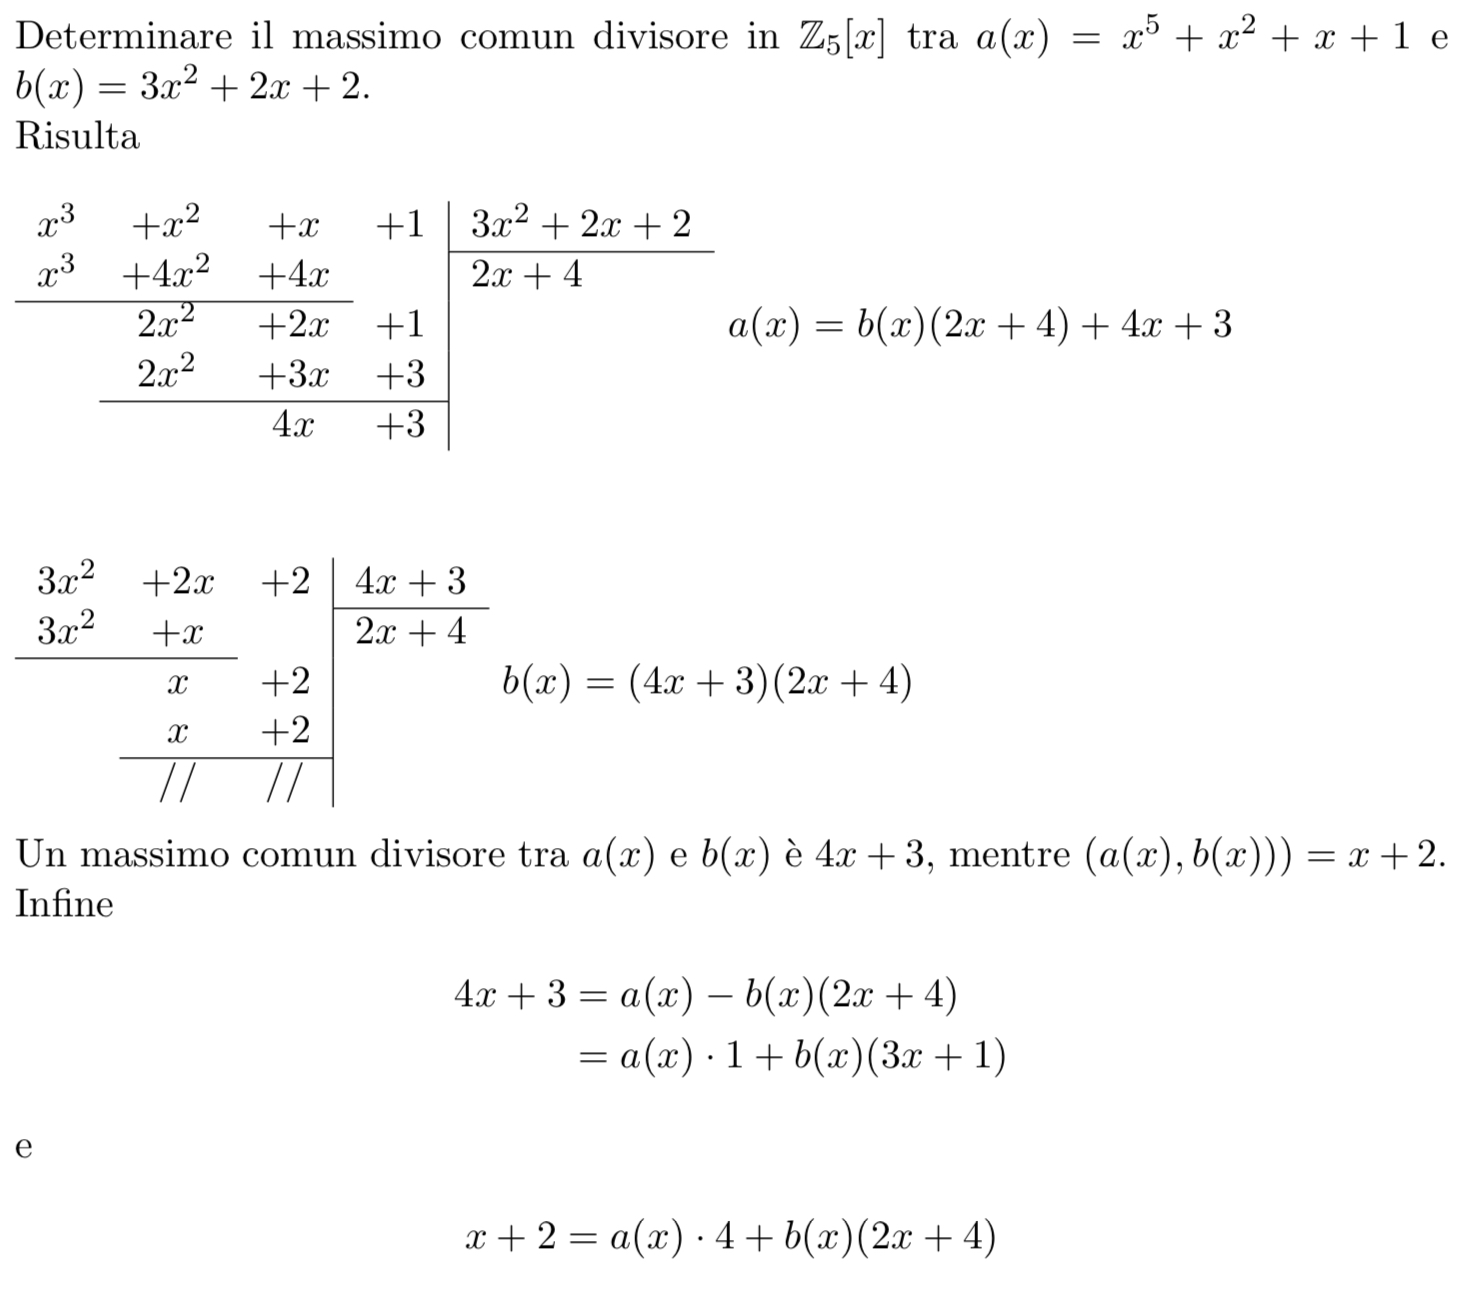
\includegraphics[width=\linewidth,scale=1]{polydiv1}
				\end{figure}	
			\end{shaded}	
			
			\begin{shaded}
				\begin{esempio}
				\end{esempio}
				\begin{figure}[H]
					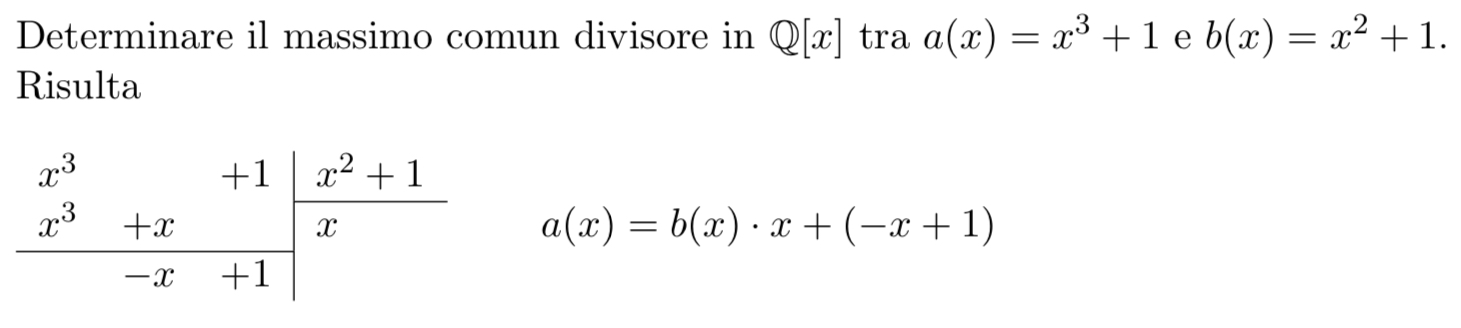
\includegraphics[width=\linewidth,scale=1]{polydiv2}
					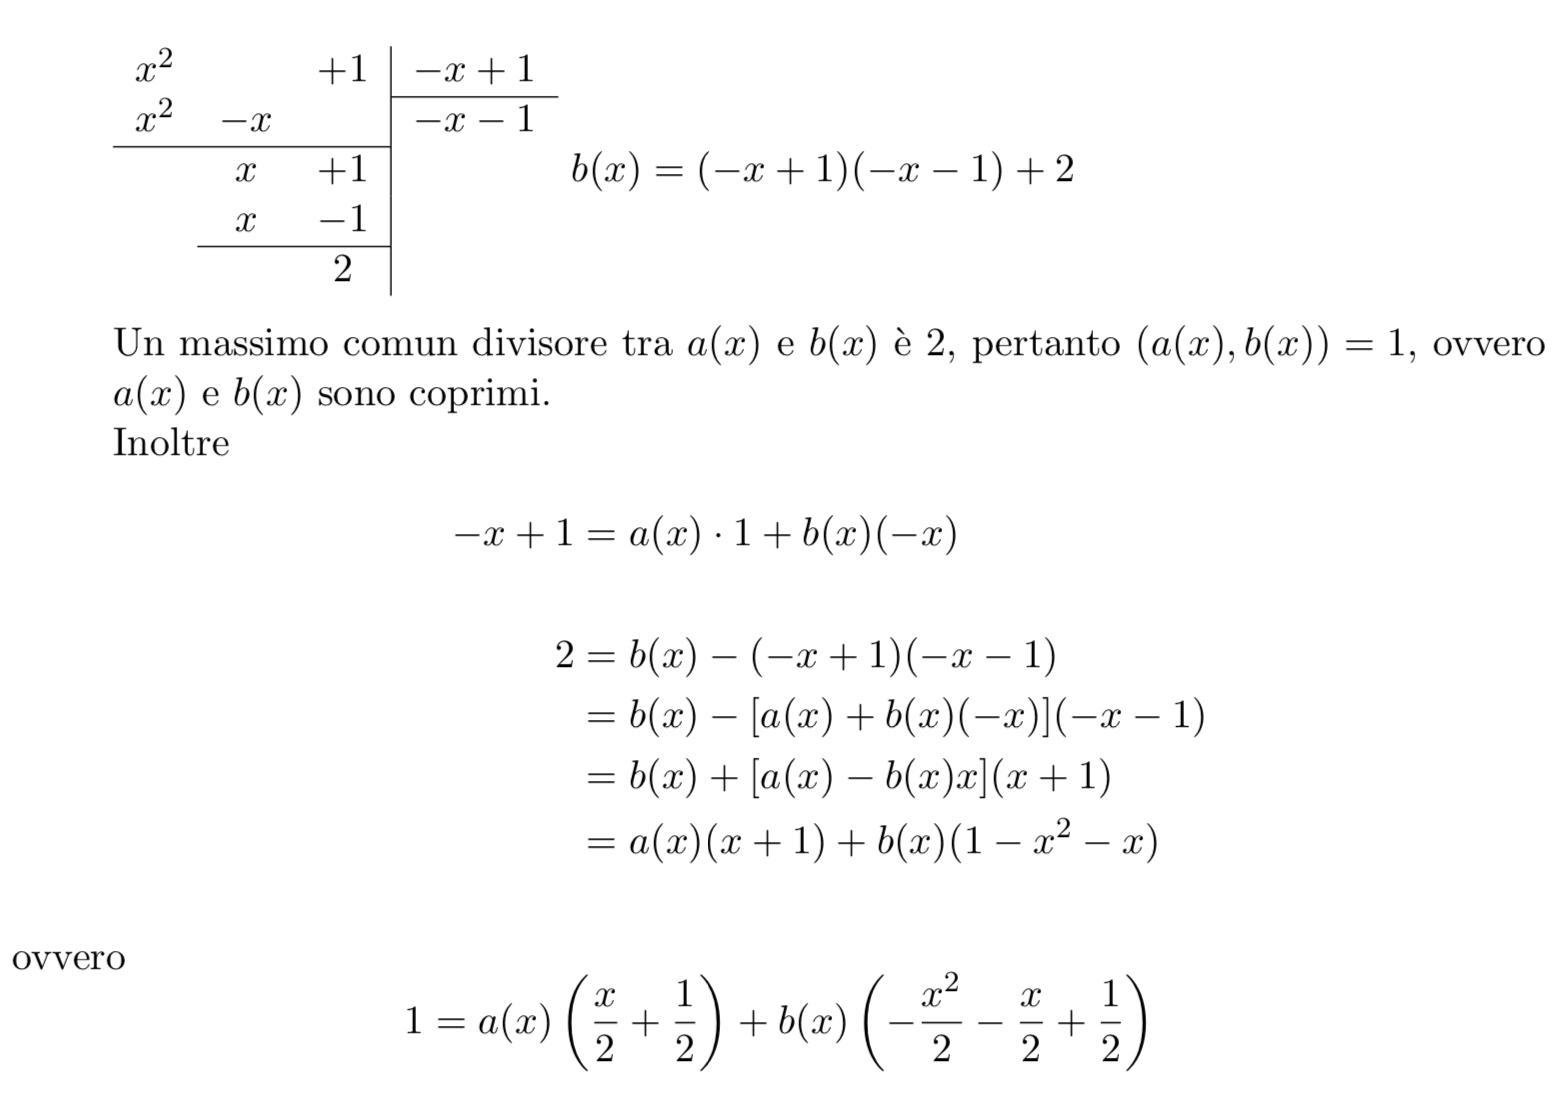
\includegraphics[width=\linewidth,scale=1]{polydiv3}
				\end{figure}	
			\end{shaded}
			
			\begin{definizione}
				Sia $a(x) \in K[x]$ un polinomio di grado $n > 0$. Si dice che $a(x)$ è un \textbf{polinomio primo} in $K[x]$ se ogni volta che $a(x) | b(x)c(x)$, con $b(x),c(x) \in K[x]$, si ha $a(x) | b(x)$ oppure $a(x) | c(x)$.
			\end{definizione}
			
			\begin{osservazione}
				Se un polinomio primo $a(x)$ divide il prodotto $n \geq 2$ polinomi, segue dalla definizione (per induzione su $n$) che $a(x)$ divida almeno uno dei fattori.
			\end{osservazione}
			
			\begin{definizione}
				Sia $a(x) \in K[x]$ un polinomio di grado $n>0$. Si dice che $a(x)$ è un polinomio irriducibile (in $K[x]$) se $a(x)$ è divisibile solo per i polinomi di grado $0$ e per i polinomi della forma $h \cdot a(x)$ con $h \in K^{*}$. In caso contrario, si dice che a(x) riducibile.
				
				Detto diversamente: il polinomio $a(x)$ è irriducibile se e solo se è fattorizzabile soltanto come
				$$a(x) = h^{-1}(ha(x)) \qquad \mbox{ con } h \in K^{*}$$
			\end{definizione}
			
			\begin{teorema}
				Un polinomio $a(x) \in K[x]$ è irriducibile se e solo se è primo.
				
				\begin{proof}
					Analoga a quella vista in $\mathbb{Z}$.
				\end{proof}
			\end{teorema}
			
			\begin{osservazione}
				La nozione di irriducibilità di un polinomio $a(x) \in K[x]$ dipende dal campo $K$ cui appartengono i coefficienti del polinomio.
				Se $K$ è un sottocampo di un campo $F$, si può riguardare $a(x)$ come polinomio in $F[x]$. Può accadere che $a(x)$ sia irriducibile in $K[x]$ ma riducibile in $F[x]$.
			\end{osservazione}
			
			\begin{shaded}
				\begin{esempio}
					Il polinomio $a(x) = x^2 -2$ è irriducibile in $\mathbb{Q}[x]$, ma è riducibile in $\mathbb{R}[x]$ perchè
					$$x^2 -2 = (x-\sqrt{2}) (x+\sqrt{2}) \quad \mbox{in} \quad \mathbb{R}[x]$$
				\end{esempio}
				\begin{esempio}
					Il polinomio $a(x) = x^2 +1$ è irriducibile in $\mathbb{Q}[x]$ e in $\mathbb{R}[x]$, ma è riducibile in $\mathbb{C}[x]$ perchè
					$$x^2 +1 = (x-i) (x+i) \quad \mbox{in} \quad \mathbb{C}[x]$$
				\end{esempio}
			\end{shaded}
			
			\begin{teorema}[Teorema della fattorizzazione unica]
				Ogni polinomio $a(x) \in K[x]$ di grado $n>0$ può essere scritto come prodotto di $s \geq 1$ polinomi irriducibili (non necessariamente distinti).
				
				Tale fattorizzazione è essenzialmente unica, nel senso che se 
				$$a(x) = p_1(x) \dots p_s(x) = q_1(x) \dots q_t(x)$$ dove i polinomi 
				$$p_i(x), q_j(x) \qquad (1 \leq i \leq s)$$ sono irriducibili, si possono ordinare i fattori in modo che $$s=t$$ e 
				$$p_1(x) = h_1q_1(x), \dots , p_s(x) = h_sq_s(x)$$
				con $h_i \in K^{*} \qquad (q \leq i \leq s)$
				
				\begin{proof}
					Da dimostrare. % TODO: da dimostrare #18
				\end{proof}
			\end{teorema}
			
			\begin{corollario}
				Ogni polinomio $a(x) \in K[x]$ di grado $n>0$ si può scrivere come 
				$$a(x) = ka_1(x) \dots a_s(x)$$
				dove $k \in K^{*}$ è il coefficiente direttore di $a(x)$ e i polinomi $a_1(x), \dots, a_s(x)$ sono monici e irriducibili. Tale scrittura è unica a meno dell'ordine.
			\end{corollario}
			

% to be continued...			
\chapter{Radici di un Polinomio}
\chapter{Costruzione di Campi}
\chapter{Permutazioni}
\chapter{Teoria dei Codici}
\chapter{Codici Lineari}
			
		
	
\end{document}